% ****** Start of file apssamp.tex ******
%
%   This file is part of the APS files in the REVTeX 4.1 distribution.
%   Version 4.1r of REVTeX, August 2010
%
%   Copyright (c) 2009, 2010 The American Physical Society.
%
%   See the REVTeX 4 README file for restrictions and more information.
%
% TeX'ing this file requires that you have AMS-LaTeX 2.0 installed
% as well as the rest of the prerequisites for REVTeX 4.1
%
% See the REVTeX 4 README file
% It also requires running BibTeX. The commands are as follows:
%
%  1)  latex apssamp.tex
%  2)  bibtex apssamp
%  3)  latex apssamp.tex
%  4)  latex apssamp.tex
%
% This file may be formatted in either the \texttt{preprint} or
% \texttt{reprint} style. \texttt{reprint} format mimics final journal output. 
% Either format may be used for submission purposes. \texttt{letter} sized paper should
% be used when submitting to APS journals.
\documentclass[%
 reprint,
superscriptaddress,
onecolumn,
% linenumbers,
notitlepage,
%groupedaddress,
%unsortedaddress,
%runinaddress,
%frontmatterverbose, 
%preprint,
%showpacs,preprintnumbers,
%nofootinbib,
%nobibnotes,
%bibnotes,
 amsmath,amssymb,
 aps,
prc,
%prb,
%rmp,
%prstab,
%prstper,
%floatfix,
]{revtex4-1}

\usepackage{graphicx}% Include figure files
\usepackage{dcolumn}% Align table columns on decimal point
\usepackage{bm}% bold math
%\usepackage{hyperref}% add hypertext capabilities
%\usepackage[mathlines]{lineno}% Enable numbering of text and display math
%\linenumbers\relax % Commence numbering lines

%\usepackage[showframe,%Uncomment any one of the following lines to test 
%%scale=0.7, marginratio={1:1, 2:3}, ignoreall,% default settings
%%text={7in,10in},centering,
%%margin=1.5in,
%%total={6.5in,8.75in}, top=1.2in, left=0.9in, includefoot,
%%height=10in,a5paper,hmargin={3cm,0.8in},
%]{geometry}


\usepackage[american]{babel}
\usepackage{amsmath}
\usepackage[version=3]{mhchem} 
% \usepackage{fixltx2e}
% \usepackage{refcount}
% \usepackage{siunitx}
% \usepackage{lastpage}
% \usepackage{textcomp}
\usepackage{mathtools}

\usepackage{xfrac}
\usepackage{lmodern}
\usepackage[hidelinks]{hyperref}
% \usepackage{cool}
% \usepackage{cancel}
\usepackage{microtype}
\usepackage{listings}
% \usepackage{mcode}
\usepackage [autostyle, english = american]{csquotes}
% \usepackage{longtable}
% \usepackage{subcaption}
\usepackage{booktabs,siunitx}
\usepackage{gensymb}
\usepackage[normalem]{ulem}



% Sin and Cos with auto-parentheses 
\newcommand{\sinp}[1]{\sin{\left( #1\right)}}
\newcommand{\cosp}[1]{\cos{\left( #1\right)}}
\newcommand{\expp}[1]{\exp{\left( #1\right)}}
\newcommand{\sinhp}[1]{\sinh{\left( #1\right)}}
\newcommand{\lnp}[1]{\ln{\left( #1\right)}}
\newcommand{\pp}[1]{\left( #1\right)}
\newcommand{\sci}[2]{ #1 \cdot 10^{#2}\ }
\newcommand{\angstrom}{\mbox{\normalfont\AA}}
\newcommand{\norm}[1]{\lVert #1 \rVert}
\newcommand{\etal}{\emph{et\,al.}} 


% To-do comments
\usepackage[colorinlistoftodos]{todonotes}
\newcommand{\comment}[1]{\todo[color=blue!20!white,inline]{ASV: #1}} 
\newcommand{\cmmnt}[1]{}


% Red highlighting quick macro
\newcommand{\textred}[1]{\textcolor{red}{ #1}}

% Sick of fighting siunitx - consistent text micro symbol
\usepackage{siunitx}
% DO NOT uncomment this!!! or else broken unicode (Âţ)
% \sisetup{math-micro=\text{µ},text-micro=µ}
% \si\micro
\newcommand{\mmicro}{\si\micro} 





\begin{document}

%\preprint{APS/123-QED}

% \title{Measurement of nuclear excitation functions for proton induced reactions  (E\texorpdfstring{$_{\text{p}}$\,=\,}{Ep = ???--55}???--55 MeV) on natural Fe}% Force line breaks with \\
\title{Measurement of nuclear excitation functions for proton induced reactions (E\texorpdfstring{$_{\text{p}}$\,=\,???--55\,}{Ep = ???--55 }MeV) on natural Fe}% Force line breaks with \\
% \thanks{A footnote to the article title}%

\author{Andrew S. Voyles}
 \email{andrew.voyles@berkeley.edu}
\affiliation{%
 Department of Nuclear Engineering, University of California, Berkeley,  Berkeley, CA 94720, USA
%  Authors' institution and/or address\\
%  This line break forced with \textbackslash\textbackslash
}% 
\author{Eric F. Matthews}%
% \author{Eric F. Matthews}%
%  \email{Second.Author@institution.edu}
\affiliation{%
 Department of Nuclear Engineering, University of California, Berkeley, Berkeley, CA 94720, USA
%  Authors' institution and/or address\\
%  This line break forced with \textbackslash\textbackslash
}%
\author{Jonathan T. Morrell}%
% \author{Eric F. Matthews}%
%  \email{Second.Author@institution.edu}
\affiliation{%
 Department of Nuclear Engineering, University of California, Berkeley, Berkeley, CA 94720, USA
%  Authors' institution and/or address\\
%  This line break forced with \textbackslash\textbackslash
}%

\author{M. Shamsuzzoha Basunia}
\affiliation{Nuclear Science Division, Lawrence Berkeley National Laboratory,  Berkeley, CA 94720, USA}
\author{Lee A. Bernstein}
\affiliation{Nuclear Science Division, Lawrence Berkeley National Laboratory,  Berkeley, CA 94720, USA}
\affiliation{%
 Department of Nuclear Engineering, University of California, Berkeley, Berkeley, CA 94720, USA
%  Authors' institution and/or address\\
%  This line break forced with \textbackslash\textbackslash
}%
% \author{Eva R. Birnbaum}
% \affiliation{Isotope Production Facility, Chemistry Division, Los Alamos National Laboratory,  Los Alamos, NM 87544, USA}
\author{Jonathan W. Engle}
 \email{jwengle@wisc.edu}
\affiliation{Department of Medical Physics, University of Wisconsin -- Madison,  Madison, WI 53705, USA}
\author{Stephen A. Graves}
\affiliation{Department of Radiation Oncology, University of Iowa,  Iowa City, IA 52242, USA}
% \author{Toshihiko ??? Kawano}
% \affiliation{Nuclear Physics Group, Theoretical Division, Los Alamos National Laboratory,  Los Alamos, NM 87544, USA}
%  \altaffiliation[Also at ]{Physics Department, XYZ University.}%Lines break automatically or can be forced with \\
\author{Amanda M. Lewis}%
% \author{Eric F. Matthews}%
%  \email{Second.Author@institution.edu}
\affiliation{%
 Department of Nuclear Engineering, University of California, Berkeley, Berkeley, CA 94720, USA
%  Authors' institution and/or address\\
%  This line break forced with \textbackslash\textbackslash
}%
\author{Alexander  Springer}%
% \author{Eric F. Matthews}%
%  \email{Second.Author@institution.edu}
\affiliation{%
 Fakult{\"a}t f{\"u}r Physik, Karlsruhe Institute of Technology, 76131 Karlsruhe, Germany
%  Authors' institution and/or address\\
%  This line break forced with \textbackslash\textbackslash
}%
% \title{Measurement of nuclear excitation functions for proton induced reactions (E\texorpdfstring{$_{\text{p}}$\,=\,}{Ep = 40--90}40--90 MeV) on natural Nb}% Force line breaks with \\
% % \thanks{A footnote to the article title}%



% \collaboration{MUSO Collaboration}%\noaffiliation
% 
% \author{Charlie Author}
% %  \homepage{http://www.Second.institution.edu/~Charlie.Author}
% \affiliation{
%  Second institution and/or address\\
%  This line break forced% with \\
% }%
% \affiliation{
%  Third institution, the second for Charlie Author
% }%
% \author{Delta Author}
% \affiliation{%
%  Authors' institution and/or address\\
%  This line break forced with \textbackslash\textbackslash
% }%
% 
% \collaboration{CLEO Collaboration}%\noaffiliation

\date{\today}% It is always \today, today,
             %  but any date may be explicitly specified

\begin{abstract}


% %
% 
%  Insert abstract text 
% 
% % 
% An article usually includes an abstract, a concise summary of the work
% covered at length in the main body of the article. 
% % \begin{description}
% % \item[Usage]
% % Secondary publications and information retrieval purposes.
% 
% % Not using PACS anymore - deprecated in favor of PhySH now?
% % \item[PACS numbers]
% % May be entered using the \verb+\pacs{#1}+ command.
% % \item[Structure]
% % You may use the \texttt{description} environment to structure your abstract;
% use the optional argument of the \verb+\item+ command to give the category of each item. 
% % \end{description}


% % Intermediate-energy proton beams are used to produce a wide range of radionuclides for use in medical treatments and research.  
% % However, reaction modeling in this energy range remains largely untested, and there is a paucity of monitor reactions in this energy range needed to establish beam characteristics  for quantitative cross section measurements.  
% % To address this need, a
% A stack  of thin Fe 
% % , Cu, and Al monitor 
% foils was irradiated with  55\,MeV and 25\,MeV proton beams at Lawrence Berkeley National Laboratory's 88-Inch Cyclotron,  to investigate the \ce{^{nat}Fe}(p,x)  nuclear reaction channels as a  pathway for low-energy production of the emerging non-standard PET radionuclides \ce{^{51}Mn} and \ce{^{52m,g}Mn}.
% % monitor for intermediate energy proton experiments and to benchmark state-of-the-art reaction model codes.
% % A stacked target of natural Nb, Cu, and Al thin foils were irradiated by 100 MeV protons at the Los Alamos National Laboratory's Isotope Production Facility.
% % The irradiation was motivated by interest in the characterization of the \ce{^{93}Nb}(p,4n)\ce{^{90}Mo} reaction as a new monitor reaction standard for intermediate-energy protons.
% A set of 34 measured  cross sections for  \ce{^{nat}Fe}(p,x), \ce{^{nat}Cu}(p,x), and  \ce{^{nat}Ti}(p,x) reactions between threshold and 55\,MeV, as well as three independent measurements of isomer branching ratios, are reported. 
% % The measurements are 
% These are useful in medical and basic science radionuclide productions at low energies. 
% % Cross sections were measured using the well-characterized 
% The
% % \ce{^{nat}Al}(p,x)\ce{^{22}Na}, \ce{^{nat}Al}(p,x)\ce{^{24}Na}, 
% \ce{^{nat}Ti}(p,x)\ce{^{46}Sc}, \ce{^{nat}Ti}(p,x)\ce{^{48}V}, \ce{^{nat}Cu}(p,x)\ce{^{62}Zn}, and \ce{^{nat}Cu}(p,x)\ce{^{63}Zn} monitor  reactions were used to
% determine proton fluence, with all activities  quantified via HPGe spectrometry.
% Variance minimization techniques were employed to reduce systematic uncertainties in proton energy and fluence, improving the reliability of these measurements. 
% The measured cross sections are shown to be in excellent agreement with  literature values where they exist, and have been measured with improved precision compared with previous measurements.
% This work also reports the first measurement for $\leq$70\,MeV protons  of the  
% \ce{^{nat}Fe}(p,x)\ce{^{49}Cr},\ce{^{51,52m,56}Mn},\ce{^{58m}Co} reactions, as well as the first measurement of the independent cross sections for    \ce{^{nat}Fe}(p,x)\ce{^{51}Cr},\ce{^{52g}Mn},\ce{^{58g}Co}.
% % \textred{\ce{^{nat}Nb}(p,x)\ce{^{82m}Rb} reaction, and of the independent cross sections for    
% % \ce{^{nat}Cu}(p,x)\ce{^{52\text{m}}Mn}, 
% % \ce{^{nat}Cu}(p,x)\ce{^{52\text{g}}Mn} and \ce{^{nat}Nb}(p,x)\ce{^{85\text{g}}Y} in the 40--90\,MeV region.}
% % .
% % \textred{
% % Due to \ce{^{nat}Si}(p,x)\ce{^{22,24}Na} contamination  by  activation of the silicone adhesive used for sealing foil packets, the \ce{^{nat}Al}(p,x)\ce{^{22}Na} and \ce{^{nat}Al}(p,x)\ce{^{24}Na}  monitor reactions  were excluded, in the interest of surety, from proton fluence determination.
% % }
% % \textred{
% % To avoid inadvertently reporting enhanced proton fluence due to
% % The effects of  \ce{^{nat}Si}(p,x)\ce{^{22,24}Na} contamination, arising from  silicone adhesive in the Kapton tape used to encapsulate the aluminum monitor foils, is also discussed as a cautionary note to future stacked-target cross section measurements.
% % strongly discouraged.
% % }
% % Comparisons against the 
% \emph{A priori} predictions of the reaction modeling codes  CoH, EMPIRE, TALYS, and ALICE are compared with experimentally measured values and used to explore the differences between codes for the
% % impact of pre-equilibrium particle emission  for the 
% % 40--90 MeV 
% \ce{^{nat}Fe}(p,x), \ce{^{nat}Cu}(p,x), and  \ce{^{nat}Ti}(p,x) reactions, illustrating that these codes fail to reproduce the deposition of angular momentum at both compound and pre-compound energies.



Theoretical models often differ significantly from measured data in their predictions of the magnitude of nuclear reactions that produce radionuclides for medical, research, and national security applications.
% Numerous reaction modeling packages can be used to calculate radionuclide production cross sections for medical, research, and national security applications. 
% However, while all of these models invoke similar physical processes, their results often differ significantly.  
In this paper, we compare \emph{a priori} predictions from several state-of-the-art reaction modeling packages (CoH, EMPIRE, TALYS, and ALICE) to cross sections measured using the stacked-target activation method.  
The experiment was performed using the LBNL 88-Inch Cyclotron with beams of 25 and 55\,MeV protons on a stack of 
% natural 
iron, copper, and titanium foils.  
% A total of 
34 excitation functions were measured from 4--55 MeV, including the first measurement of the independent cross sections for \ce{^{nat}Fe}(p,x)\ce{^{49,51}Cr}, \ce{^{51,52m,52g,56}Mn}, and \ce{^{58m,58g}Co}.  
All of the models, using default input parameters to assess their predictive capabilities,  failed to reproduce the isomer-to-ground state ratio for 
% many  
reaction channels at 
% both 
compound and pre-compound energies, suggesting issues in modeling the deposition or distribution of angular momentum in these residual nuclei.  



% \begin{description}
% \item[Usage]
% Secondary publications and information retrieval purposes.
% \item[PACS numbers]
% May be entered using the \verb+\pacs{#1}+ command.
% \item[Structure]
% You may use the \texttt{description} environment to structure your abstract;
% use the optional argument of the \verb+\item+ command to give the category of each item. 
% \end{description}



\end{abstract}

% Not using PACS anymore - deprecated in favor of PhySH now?
% \pacs{Valid PACS appear here}% PACS, the Physics and Astronomy
                             % Classification Scheme.
%\keywords{Suggested keywords}%Use showkeys class option if keyword
                              %display desired
\maketitle

%\tableofcontents

%%
%%  To-do list for comments
%%
\listoftodos




\section{\label{sec:intro_fe}Introduction}



Clinical practice of nuclear medicine is rapidly growing with the inclusion of a broader array of radiopharmaceuticals. 
Future growth is anticipated, given the pre-clinical success of many  new and emerging radionuclides. 
Although the physical and chemical properties of these novel radionuclides tend to be
% The next generation of nuclear medicine 
% % would appear to be based upon 
% is likely to involve the production of novel, emerging radionuclides\,\cite{Qaim201731}. 
% % The targeted and personalized nature of therapy and imaging applications using these novel radionuclides  
% These make possible an improvement in clinical practice, offering many patients the possibility for better survival rates and quality lives, and informing researchers in their quest to develop new treatments\,\cite{Mulford2005,Muller2014}.
% While the chemical and radioactive decay properties of many of these radionuclides are 
well-established, their broad-scale  clinical applications are reliant upon well-characterized nuclear data to facilitate 
% large-scale   
production. 
% 
% 
% 
% The future of nuclear medicine would appear to be the paradigm of personalized medicine --- targeted radionuclide therapy to spare healthy tissue\,\cite{Mulford2005,Qaim201731}, and theranostic medicine, which pairs an imaging isotope with a therapeutic isotope (frequently, of the same element), to provide simultaneous, real-time dose delivery and verification, leading to drastic reductions in prescribed patient dose\,\cite{Muller2014,Bentzen2005,Srivastava2012}. 
% Other variants of theranostic medicine exist, including pre-imaging for treatment planning, or delivery of a single compound with different radioelements for imaging/therapy where the inter-element biodistribution has been validated.  
% Change up the next sentance a bit
% Novel applications are being explored for several radionuclides whose production methodologies are not established, but their production requires accurate, high-fidelity cross section data.
%\,\cite{Qaim201731}. 
% Many of these applications focus on theranostics, the use of chemically identical (or similar) imaging and therapeutic radiopharmaceuticals for treatment of disease. 
One particular set of  emerging radionuclides are 
% the various 
positron-emitting isotopes of manganese, which have been identified as having potential for a range of diagnostic applications\,\cite{J.2013,Graves2015,Lewis2015,PhysRevC.96.014613,Wooten2017,Hernandez2017}.
In particular, a significant interest has been expressed in producing the emerging radionuclides \ce{^{51}Mn} for clinical use in quantitative positron emission tomography (PET) studies, as well as  \ce{^{52g}Mn} for pre-clinical imaging of neural and immune processes via PET\,\cite{Graves2016}. 




Manganese radionuclides are desirable for radiopharmaceutical applications, as 
% manganese is a 
% the element is chemically versatile,  biologically relevant, and essential in trace quantities. 
% Manganese 
they possess well-established biochemistry, and have been 
% proven to be 
chelated 
% well 
by the complexing agent DOTA for tracking monoclonal antibodies with high biostability at neutral pH\,\cite{Graves2015}.
\ce{^{52}Mn} ($t_{1/2}$ = 5.591$~\pm~$0.003\,d, $I_{\beta^+}$ = 29.4\%, $E_{\beta\text{, avg}}$ = 0.242\,MeV\,\cite{Dong2015}) has been shown to be useful for immuno-PET applications, 
% with its rapid blood clearance 
offering the possibility for imaging within minutes of injection,
% \,\cite{Dong2015}.
% Its lifetime facilitates regional production and  allows for immunoPET imaging up to 2--3 weeks after administration, giving \ce{^{52}Mn} a longer duration for useful 
% making it more useful 
making it highly suitable for pre-clinical imaging as a longer-lived complement   to the more established immuno-PET agents \ce{^{89}Zr} and   \ce{^{64}Cu}.  
% Furthermore, \ce{^{52}Mn}  has high uptake in the heart, liver, kidneys, and pancreas, making it a useful diagnostic agent for pancreatic $\beta$-cell, insulinoma, and porphysome imaging\,\cite{Graves2015}. 
However, its  long half-life and unfavorable high-energy decay gamma-rays 
% (notably, its  744.233\,keV [$I_\gamma = 90.0\,\pm\,1.2\%$], 935.544\,keV [$I_\gamma = 94.5\,\pm\,1.3\%$], and 1434.092\,keV [$I_\gamma = 100.0 \pm 1.4\%$] lines) 
make it undesirable for clinical applications.
% , but easily shipped worldwide and highly suitable for pre-clinical imaging\,\cite{Dong2015}.
The short half-life of the  \ce{^{52m}Mn} isomer ($t_{1/2}$ = 21.1$~\pm~$0.2\,min)
% , $I_{\beta^+}$\,=\,96.6\%, $E_{\beta\text{,avg}}$ = 1.172\,MeV) offers a much stronger positron emission branch than \ce{^{52g}Mn}, but its short lifetime 
makes production and handling difficult, and with a  high-intensity gamma emission (1434.06\,keV, $I_\gamma = 98.2~\pm~0.5\%$),  
\ce{^{52m}Mn} is similarly undesirable for clinical applications\,\cite{Dong2015}.
% contributes significantly to patient dose\,\cite{Dong2015}.
% Another emerging manganese radionuclide is 
In contrast, \ce{^{51}Mn} ($t_{1/2}$ = 46.2$~\pm~$0.1\,min, $I_{\beta^+}$ = 96.86\%, $E_{\beta\text{, avg}}$ = 0.964\,MeV\,\cite{Wang2017}), 
% whose short lifetime makes it 
is more clinically suitable for rapid metabolic studies.
% \ce{^{51}Mn} has a comparable positron branch and energy to \ce{^{52m}Mn} and is more suitable for clinical use than the soft positron emissions of \ce{^{52g}Mn}. 
% In addition, 
\ce{^{51}Mn} lacks any strong decay gamma-rays (its longer-lived daughter \ce{^{51}Cr} [$t_{1/2}$ = 27.704$~\pm~$0.003\,d] has only a single  320.0284\,keV [$I_\gamma = 9.910~\pm~0.010\%$] line), making it the best choice of these radionuclides for clinical imaging.
% ,\cite{Wang2017}.



Developing production of these radionuclides requires well-characterized cross section data, or predictive models when such data have not been measured.   
% However, the m
Modeling of nuclear reactions in 
% this 
the A=40--70 mass region presents numerous challenges including uncertainties in nuclear level densities as a function of spin due to the opening of the $f_{7/2}$ orbital and the presence of enhanced $\gamma$-strength at low energies\,\cite{Voinov2004a,Algin2008,Algin2007}.  
% As 
Therefore, as part of a larger campaign to address deficiencies in cross-cutting nuclear data needs, our group has
% performed a   measurement of 
measured the   nuclear excitation functions of the radionuclides \ce{^{51}Mn},   \ce{^{52m}Mn}, and \ce{^{52g}Mn} from proton-induced reactions on Fe.
% natural iron.
% This was carried out 
% in a
% using 
We used the thin-foil stacked-target technique to study proton-induced reactions on 
% experiment, using proton irradiation of 
% natural iron foils 
% iron 
Fe foils of natural isotopic abundance with 
% titanium 
Ti and 
% copper 
Cu monitor foils.
% While recent work has been performed in the 40--100\,MeV energy region, t
This work 
% seeks to 
complements 
% these measurements 
earlier measurements using 40--100\,MeV protons  and extends them down to reaction thresholds,  to investigate the feasibility of production using the international network   of low-energy medical cyclotrons\,\cite{Graves2016}. 
Furthermore, 
% we are able to use a portion of the data we measured to gain insight into the role of 
we used our measured data to probe the role of angular momentum in the transitional energy region between compound and direct reactions since both the ground and long-lived isomeric states in \ce{^{52}Mn} were populated.  






% While these efforts have been targeted towards the production cross section of the \ce{^{51,52g,52m}Mn} PET isotopes (as well as other emerging medical radionuclides produced in these irradiations), these measurements offer insight into the spin distribution of excited nuclear states, in the 5--55 MeV range.


% In addition to the interest in the production of\ce{^{51,52g,52m}Mn} for PET research

% While these efforts have been motivated by the production cross section of the
In addition to their interest for PET studies, the \ce{^{51,52g,52m}Mn} excitation functions 
% radionuclides for PET studies, this experiment 
offer an opportunity to study the distribution of angular momentum in compound nuclear and direct pre-equilibrium reactions via observation of the \ce{^{52m}Mn} ($t_{1/2}$ = 21.1$~\pm~$0.2\,min; J$^\pi=2^+$) to \ce{^{52g}Mn} ($t_{1/2}$ = 5.591$~\pm~$0.003\,d; J$^\pi=6^+$)   ratio\,\cite{Dong2015,Wang2017}.
Measurements of isomer-to-ground state ratios have been used for over 20\,years to probe the spin distribution of excited nuclear states in the A\,$\approx$\,190 region\,\cite{PhysRevC.73.034613,PhysRevC.45.1171}.
These measurements also provide an opportunity to benchmark 
% a range of cross section data invaluable to not only the medical isotope production community, but  also serve to measure the spin distribution in \textred{f$_{7/2}$} subshell nuclei via the observation of isomer-to-ground state ratios, and  as new data to improve 
the predictive capabilities of  reaction modeling codes used for nuclear reaction evaluations and the way in which they implement the underlying physical reaction mechanisms.  
% codes. 
% In addition, these experiments provide valuable insight into the challenges  involved in precision cross section data measurements. 



% A set of measured cross sections for the various natFe(p,x), natTi(p,x), and natCu(p,x) reactions between 5–55 MeV, as well as independent measurements of isomer branching ratios, are reported.
% Figure 3 shows the 52mMn(2+)/52gMn(6+) isomer-to-ground state branching ratio for the naFe(p,αn) reaction, calculated using TALYS-v1.8 over the 20 - 55 MeV range spanned by the foil stack. It is possible to use this measurement to infer the spin cut-off σ2, the width of the angular momentum distribution of the level density [6], [7]. The isomer-to-ground state ratio lends insight into equilibrium / pre-equilibrium nature of reactions in this energy region, useful when attempting to minimize dose from an unwanted isomer/ground state of a medical radionuclide.



% While this might seem obvious, the contributions to the slowing of the beam due to the adhesive has often been neglected in much work performed to date. While plays a limited role at high beam energies, it becomes increasingly important for proton energies below 25 MeV. 




% In addition to providing a potentially highly-valuable beam monitor, the Nb(p,x) reactions offer an opportunity to study the angular momentum deposition via pre-equilibrium reactions and the spin distribution in f$_{7/2}$ subshell nuclei via the observation of isomer-to-ground state ratios.  





% lee stuff:
% 
% In addition to the interest in the production of 51,52 Mn for PET research, this experiment offered
% an opportunity to study the distribution of angular momentum in compound nuclear and direct
% pre-equilibrium reactions via observation of the 52g Mn (t ½ =5.591±0.003 d; J π =6 + ) to 52m Mn
% (t ½ =21.1±0.2 m; J π =2 + ) ratio. These results indicated were presented at the University of Oslo in
% May 2017 5 and indicate that the constant
% temperature nuclear level density model
% which has had the greatest success at
% reproducing most low-energy nuclear
% reaction data fails to reproduce the
% deposition of angular momentum at both
% compound and pre-compound energies
% (see figure 3). This result will be
% discussed in greater detail in Mr. Andrew
% Voyles’ doctoral dissertation, which is
% expected to be completed by May 2018.
% 
% An important outcome from this work has an appreciation for the role played by the latex
% adhesive on the Kapton tape used to contain the individual stacked targets. While this might
% seem obvious, the contributions to the slowing of the beam due to the adhesive has been
% neglected in work performed at LANL-IPF to date. While this is expected to play a limited role
% at high beam energies, it becomes increasingly important for proton energies below 25 MeV.








% This sample document demonstrates proper use of REV\TeX~4.1 (and
% \LaTeXe) in mansucripts prepared for submission to APS
% journals. Further information can be found in the REV\TeX~4.1
% documentation included in the distribution or available at
% \url{http://authors.aps.org/revtex4/}.
% 
% When commands are referred to in this example file, they are always
% shown with their required arguments, using normal \TeX{} format. In
% this format, \verb+#1+, \verb+#2+, etc. stand for required
% author-supplied arguments to commands. For example, in
% \verb+\section{#1}+ the \verb+#1+ stands for the title text of the
% author's section heading, and in \verb+\title{#1}+ the \verb+#1+
% stands for the title text of the paper.
% 
% Line breaks in section headings at all levels can be introduced using
% \textbackslash\textbackslash. A blank input line tells \TeX\ that the
% paragraph has ended. Note that top-level section headings are
% automatically uppercased. If a specific letter or word should appear in
% lowercase instead, you must escape it using \verb+\lowercase{#1}+ as
% in the word ``via'' above.

\section{\label{sec:experimental_fe}Experimental Methods and Materials}


The work described herein follows the  methods utilized in our recent work and established by Graves \etal\ 
% for the measurement of cross sections in stacked target irradiations   
for monitor reaction characterization of beam energy and fluence in stacked target irradiations\,\cite{Voyles2018a,Graves2016}.
% 
% Make sure to add this back in for the journal article
% 
% 
Preliminary results  were reported in a Master's thesis \cite{springer2017investigation}; here we report the final analysis of that work.
% of one co-author, but the conclusive results of this work are described here\,\cite{springer2017investigation}.  
Unless otherwise stated, all values are presented herein as mean $\pm$ SD, or as the calculated result $\pm$ half the width of a 68\% confidence interval.



\subsection{\label{sec:target_design_fe}Stacked-target design}


We constructed a pair of target stacks 
% were constructed 
for this work,
% , due to the large energy range desired to be spanned.
one stack covering the 55--20\,MeV range and the other  25--0\,MeV.
% , in order to 
This minimized the systematic uncertainties associated with significant degradation of beam energy, and
% In addition, the complementary  energy  of the  stacks helps build confidence  through 
included multiple overlapping measurements between 20--25\,MeV as a consistency check between the stacks.
% to build confidence in the results. 
% A stacked-target design was utilized for this work in order that the (p,x) cross sections for each reaction channel could be measured at multiple energy positions in a single irradiation\,\cite{Cumming1963}. 
% For targets, a
A series of nominal 25\,\mmicro m \ce{^{nat}Fe} foils (99.5\%, lot \#LS470411), 25\,\mmicro m \ce{^{nat}Ti} foils (99.6\%, lot \#LS471698), and 25\,\mmicro m \ce{^{nat}Cu} foils (99.95\%, lot \#LS471698) were used (all from Goodfellow Corporation, Coraopolis, PA 15108, USA) as targets.
In each stack, seven foils 
% of each metal 
were cut down to 2.5$\times$2.5\,cm squares and spatially characterized 
% --- for each foil, length and width measurements were taken 
at four different locations using a digital caliper and micrometer (Mitutoyo America Corp.).
% , thickness measurements were taken at four different locations using a digital micrometer (Mitutoyo America Corp.), and 
Four mass measurements were performed using an analytical balance 
% after cleaning the foils with isopropyl alcohol.
% Using these length, width, and mass readings, the 
in order to determine their areal density. 
% and its uncertainty 
% (in mg/cm$^2$).
% for each foil was calculated.
% , along with the propagated uncertainty in areal density.
% The foils were tightly sealed into \enquote{packets} using two pieces of  3M 1205-Series Kapton polyimide film tape --- each piece of tape consists of 38.1 \mmicro m of an acrylic adhesive (nominal 4.49 mg/cm$^2$) on 25.4 \mmicro m of a polyimide backing (nominal 3.61 mg/cm$^2$).
The foils were  sealed into \enquote{packets} using two pieces of  3M 5413-Series Kapton polyimide film tape 
% --- each piece of tape consists 
consisting of 43.2 \mmicro m of a silicone adhesive (nominal 4.79\,mg/cm$^2$) on 25.4 \mmicro m of a polyimide backing (nominal 3.61\,mg/cm$^2$).
The sealed foils were mounted over the hollow center of  1.5875 mm-thick aluminum frames.
Plates of 6061 aluminum alloy  served as proton energy degraders  between energy positions.
% One \ce{^{nat}Fe}, one \ce{^{nat}Cu}, and one \ce{^{nat}Ti} mounted foil were bundled together using baling wire for each energy position.
The target box, seen in \autoref{fig:fe_target_stack}, is machined from 6061 aluminum alloy and mounts on the end of an electrically-isolated beamline.
The specifications of both target stacks 
% designs for this work are presented 
are in \autoref{tab:fe_stack_table} of 
% Appendix 
\ref{sec:fe_stack_design}.



\begin{figure}[ht]
 \centering
 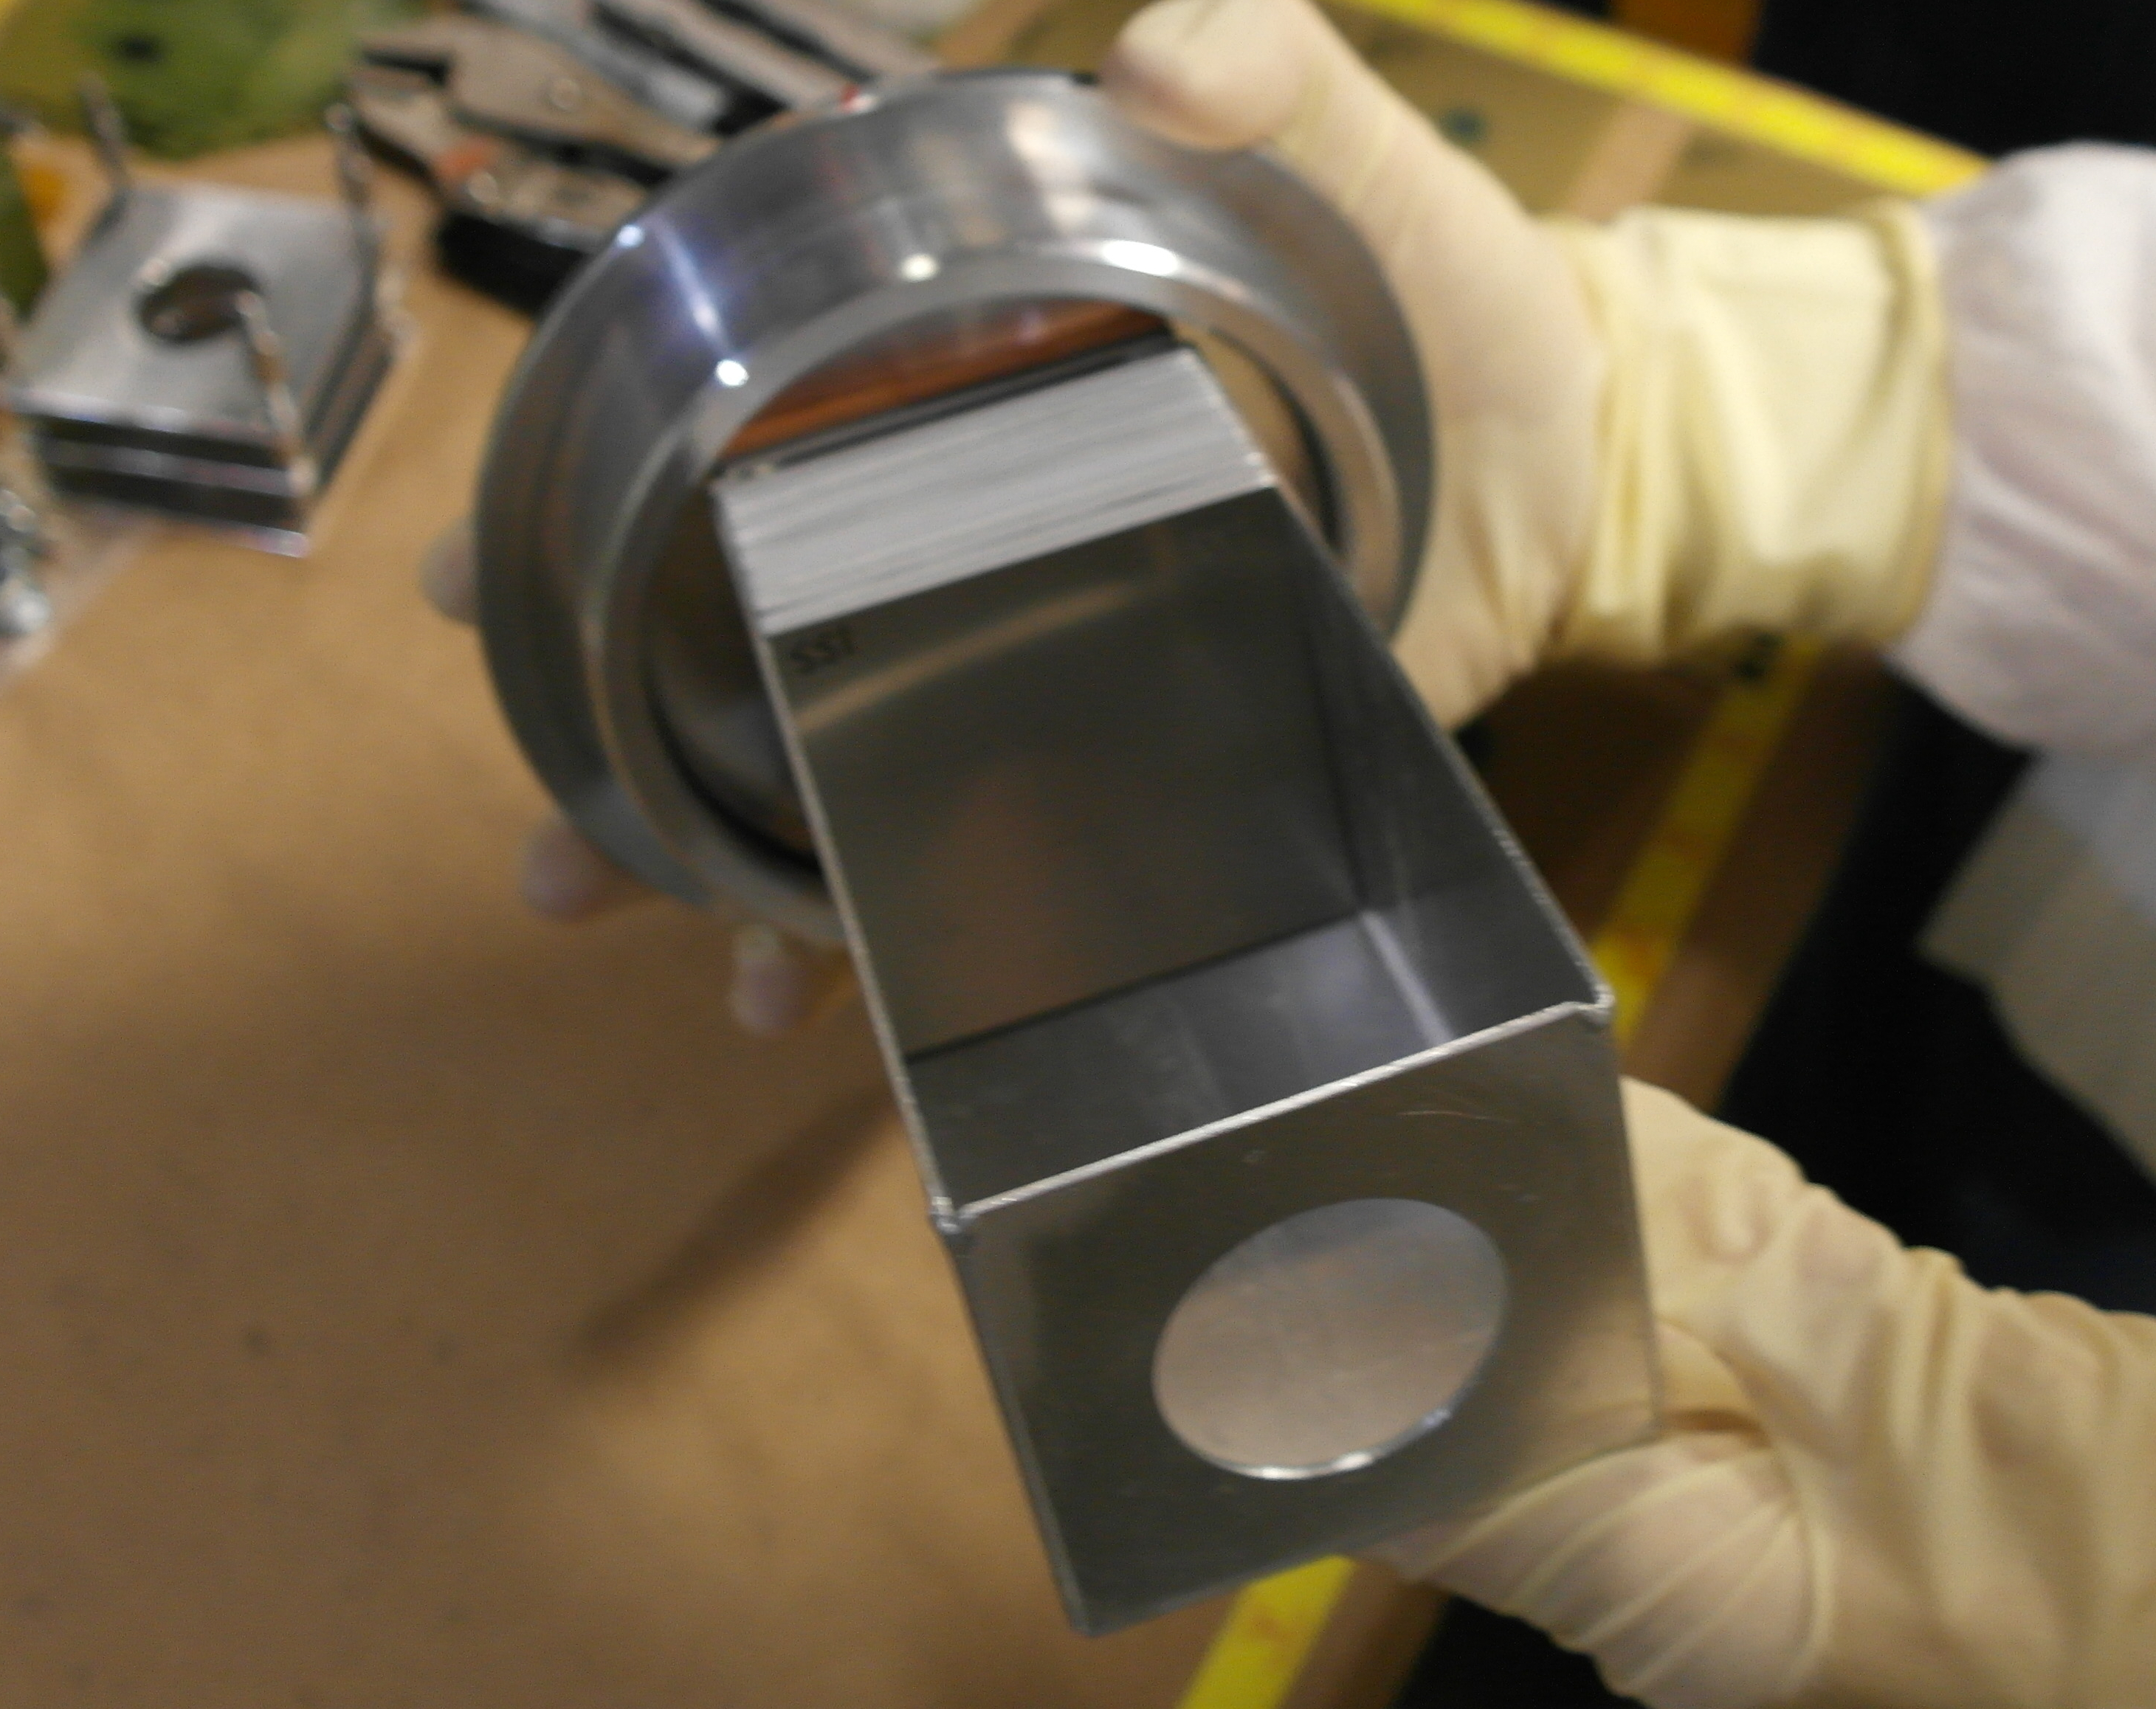
\includegraphics[width=0.45\textwidth]{./figures/SAM_2494.JPG}
 % IMG_1975.JPG: 3264x2448 pixel, 72dpi, 115.15x86.36 cm, bb=0 0 3264 2448
 \caption{\label{fig:fe_target_stack}Photograph of the assembled 25\,MeV target stack.
%  , before it was mounted in the beamline. 
 The proton beam enters through the circular entrance in the foreground, and the upstream stainless steel profile monitor (SS-5) is visible at the front of the stack.}
\end{figure}

% Separate tables
% 
% % Please add the following required packages to your document preamble:
% % \usepackage{booktabs}
% \begin{table}
% \centering
% \caption{Specifications of the  target stack design in the present work. The proton beam enters the stack upstream of the 249.8 \mmicro m SS profile monitor, and is transported through the stack in the order presented here. The 6061 aluminum degraders have a measured density of approximately 2.80 g/cm$^3$. Their areal densities were determined using the variance minimization techniques described  in this work  and the earlier paper by Graves \etal\\,\cite{Graves2016}. At both the front and rear of the target stack's foils, a 316 stainless steel foil is inserted to serve as a beam profile monitor --- after end-of-bombardment (EoB), decay radiation emitted from these activated stainless steel foils were used to develop radiochromic film (Gafchromic EBT3), revealing the spatial profile of the beam entering and exiting the stack.}
% \label{tab:fe_stack_table}
% \small
% \begin{tabular}{@{}llll@{}}
% \toprule
% % Target Layer       & Nominal Thickness & Measured thickness (mg/cm\textasciicircum 2) & Thickness Uncertainty (\%) \\ \midrule
% Target layer       & \begin{tabular}[c]{@{}l@{}}Measured \\ thickness\end{tabular} & \begin{tabular}[c]{@{}l@{}}Measured areal\\density (mg/cm$^2$)\end{tabular} & \begin{tabular}[c]{@{}l@{}}Areal density \\ uncertainty (\%)\end{tabular} \\ \midrule
% SS profile monitor SS-5 & 130.94 \mmicro m                                              & 100.57                                                                      & 0.17                                                                      \\
% Fe-08                   & 26.25 \mmicro m                                               & 19.69                                                                       & 0.17                                                                      \\
% Ti-14                   & 25.01 \mmicro m                                               & 10.87                                                                       & 0.36                                                                      \\
% Cu-14                   & 24.01 \mmicro m                                               & 17.49                                                                       & 0.40                                                                      \\
% Al Degrader E-09        & 256.5 \mmicro m                                               & --                                                                          & --                                                                        \\
% Fe-09                   & 26.5 \mmicro m                                                & 19.90                                                                       & 0.09                                                                      \\
% Ti-15                   & 23.81 \mmicro m                                               & 10.97                                                                       & 0.11                                                                      \\
% Cu-15                   & 21.81 \mmicro m                                               & 17.63                                                                       & 0.46                                                                      \\
% Al Degrader H-01        & 127.49 \mmicro m                                              & --                                                                          & --                                                                        \\
% Fe-10                   & 26.5 \mmicro m                                                & 19.84                                                                       & 0.11                                                                      \\
% Ti-16                   & 24.6 \mmicro m                                                & 10.96                                                                       & 0.32                                                                      \\
% Cu-16                   & 22.01 \mmicro m                                               & 17.22                                                                       & 0.25                                                                      \\
% Fe-11                   & 27.26 \mmicro m                                               & 19.96                                                                       & 0.17                                                                      \\
% Ti-17                   & 25.01 \mmicro m                                               & 10.88                                                                       & 0.25                                                                      \\
% Cu-17                   & 29 \mmicro m                                                  & 21.91                                                                       & 0.33                                                                      \\
% Fe-12                   & 27.01 \mmicro m                                               & 20.03                                                                       & 0.12                                                                      \\
% Ti-18                   & 25.01 \mmicro m                                               & 11.00                                                                       & 0.87                                                                      \\
% Cu-18                   & 28.75 \mmicro m                                               & 22.33                                                                       & 0.14                                                                      \\
% Fe-013                  & 26.25 \mmicro m                                               & 20.05                                                                       & 0.16                                                                      \\
% Ti-19                   & 26.6 \mmicro m                                                & 11.01                                                                       & 0.22                                                                      \\
% Cu-19                   & 28.75 \mmicro m                                               & 22.32                                                                       & 0.19                                                                      \\
% Fe-14                   & 25.75 \mmicro m                                               & 20.11                                                                       & 0.19                                                                      \\
% Ti-20                   & 27.01 \mmicro m                                               & 11.06                                                                       & 0.35                                                                      \\
% Cu-20                   & 28.26 \mmicro m                                               & 22.34                                                                       & 0.28                                                                      \\
% SS profile monitor SS-6 & 131.5 \mmicro m                                               & 100.99                                                                      & 0.17                                                                      \\
%  \bottomrule
% \end{tabular}
% \end{table}
% 
% 
% 
% 
% % Please add the following required packages to your document preamble:
% % \usepackage{booktabs}
% \begin{table}
% \centering
% \caption{Specifications of the  target stack design in the present work. The proton beam enters the stack upstream of the 249.8 \mmicro m SS profile monitor, and is transported through the stack in the order presented here. The 6061 aluminum degraders have a measured density of approximately 2.80 g/cm$^3$. Their areal densities were determined using the variance minimization techniques described  in this work  and the earlier paper by Graves \etal\\,\cite{Graves2016}. At both the front and rear of the target stack's foils, a 316 stainless steel foil is inserted to serve as a beam profile monitor --- after end-of-bombardment (EoB), decay radiation emitted from these activated stainless steel foils were used to develop radiochromic film (Gafchromic EBT3), revealing the spatial profile of the beam entering and exiting the stack.}
% \label{tab:fe_stack_table2}
% \small
% \begin{tabular}{@{}llll@{}}
% \toprule
% % Target Layer       & Nominal Thickness & Measured thickness (mg/cm\textasciicircum 2) & Thickness Uncertainty (\%) \\ \midrule
% Target layer       & \begin{tabular}[c]{@{}l@{}}Measured \\ thickness\end{tabular} & \begin{tabular}[c]{@{}l@{}}Measured areal\\density (mg/cm$^2$)\end{tabular} & \begin{tabular}[c]{@{}l@{}}Areal density \\ uncertainty (\%)\end{tabular} \\ \midrule
% SS profile monitor SS-3 & 130.9 \mmicro m                                               & 100.48                                                                      & 0.17                                                                      \\
% Fe-01                   & 25.75 \mmicro m                                               & 20.22                                                                       & 0.21                                                                      \\
% Ti-01                   & 25.88 \mmicro m                                               & 11.09                                                                       & 0.16                                                                      \\
% Cu-01                   & 28.81 \mmicro m                                               & 22.40                                                                       & 0.11                                                                      \\
% Al Degrader A-1         & 2.24 mm                                                       & --                                                                          & --                                                                        \\
% Fe-02                   & 25.5 \mmicro m                                                & 19.91                                                                       & 0.13                                                                      \\
% Ti-02                   & 25.74 \mmicro m                                               & 10.94                                                                       & 0.24                                                                      \\
% Cu-02                   & 28.75 \mmicro m                                               & 22.32                                                                       & 0.40                                                                      \\
% Al Degrader A-2         & 2.24 mm                                                       & --                                                                          & --                                                                        \\
% Fe-03                   & 25.25 \mmicro m                                               & 20.00                                                                       & 0.27                                                                      \\
% Ti-03                   & 25.91 \mmicro m                                               & 11.25                                                                       & 0.15                                                                      \\
% Cu-03                   & 28.86 \mmicro m                                               & 22.49                                                                       & 0.20                                                                      \\
% Al Degrader C-1         & 0.97 mm                                                       & --                                                                          & --                                                                        \\
% Fe-04                   & 25.25 \mmicro m                                               & 19.93                                                                       & 0.33                                                                      \\
% Ti-04                   & 25.84 \mmicro m                                               & 10.91                                                                       & 0.18                                                                      \\
% Cu-04                   & 28.78 \mmicro m                                               & 22.38                                                                       & 0.29                                                                      \\
% Al Degrader C-2         & 0.97 mm                                                       & --                                                                          & --                                                                        \\
% Fe-05                   & 25.64 \mmicro m                                               & 20.02                                                                       & 0.24                                                                      \\
% Ti-05                   & 25.86 \mmicro m                                               & 10.99                                                                       & 0.30                                                                      \\
% Cu-05                   & 28.77 \mmicro m                                               & 22.35                                                                       & 0.12                                                                      \\
% Al Degrader C-3         & 0.97 mm                                                       & --                                                                          & --                                                                        \\
% Fe-06                   & 25.75 \mmicro m                                               & 20.21                                                                       & 0.26                                                                      \\
% Ti-06                   & 25.5 \mmicro m                                                & 11.15                                                                       & 0.23                                                                      \\
% Cu-06                   & 28.83 \mmicro m                                               & 22.43                                                                       & 0.10                                                                      \\
% Al Degrader C-4         & 0.97 mm                                                       & --                                                                          & --                                                                        \\
% Fe-07                   & 25.76 \mmicro m                                               & 19.93                                                                       & 0.19                                                                      \\
% Ti-07                   & 25.75 \mmicro m                                               & 11.17                                                                       & 0.33                                                                      \\
% Cu-07                   & 28.76 \mmicro m                                               & 22.34                                                                       & 0.24                                                                      \\
% Al Degrader H-02        & 127.04 \mmicro m                                              & 34.51                                                                       & 0.20                                                                      \\
% SS profile monitor SS-4 & 131.21 \mmicro m                                              & 101.25                                                                      & 0.16                                                                     \\
%  \bottomrule
% \end{tabular}
% \end{table}

% % Combined table
% % Please add the following required packages to your document preamble:
% % \usepackage{booktabs}
% \begin{table*}
% \centering
% \caption{Specifications of the 25\,MeV and 55\,MeV target stack designs in the present work. The proton beam enters the stack upstream of the SS-5 and SS-3 profile monitors, respectively, and travels through the stack in the order presented here. The 6061 aluminum degraders have a measured density of approximately 2.68 $\pm$ 0.03 g/cm$^3$. Their areal densities were determined using the variance minimization techniques described  in this work  and an earlier paper\,\cite{Voyles2018a}. 
% % the earlier paper by Graves \etal\\,\cite{Graves2016}.
% A 316 stainless steel foil is inserted at both the front and rear of each target stack as a monitor of the beam's spatial profile, by developing radiochromic film (Gafchromic EBT3) after end-of-bombardment (EoB).}
% \label{tab:fe_stack_table}
% \small
% \resizebox{\textwidth}{!}{%
% \begin{tabular}{@{}llll|llll@{}}
% \toprule
% % Target Layer       & Nominal Thickness & Measured thickness (mg/cm\textasciicircum 2) & Thickness Uncertainty (\%) \\ \midrule
% 25\,MeV Target layer            & \begin{tabular}[c]{@{}l@{}}Measured \\ thickness\end{tabular} & \begin{tabular}[c]{@{}l@{}}Measured\\areal density\\(mg/cm$^2$)\end{tabular} & \begin{tabular}[c]{@{}l@{}}Uncertainty \\ in areal\\ density  (\%)\end{tabular} & 55\,MeV Target layer            & \begin{tabular}[c]{@{}l@{}}Measured \\ thickness\end{tabular} & \begin{tabular}[c]{@{}l@{}}Measured\\areal density\\(mg/cm$^2$)\end{tabular} & \begin{tabular}[c]{@{}l@{}}Uncertainty \\ in areal\\ density  (\%)\end{tabular} \\
% \midrule
% SS profile monitor SS-5 & 130.94 \mmicro m                                              & 100.57                                                                      & 0.17                                                                      & SS profile monitor SS-3 & 130.9 \mmicro m                                               & 100.48                                                                      & 0.17                                                                      \\
% Fe-08                   & 26.25 \mmicro m                                               & 19.69                                                                       & 0.17                                                                      & Fe-01                   & 25.75 \mmicro m                                               & 20.22                                                                       & 0.21                                                                      \\
% Ti-14                   & 25.01 \mmicro m                                               & 10.87                                                                       & 0.36                                                                      & Ti-01                   & 25.88 \mmicro m                                               & 11.09                                                                       & 0.16                                                                      \\
% Cu-14                   & 24.01 \mmicro m                                               & 17.49                                                                       & 0.40                                                                      & Cu-01                   & 28.81 \mmicro m                                               & 22.40                                                                       & 0.11                                                                      \\
% Al Degrader E-09        & 256.5 \mmicro m                                               & --                                                                          & --                                                                        & Al Degrader A-1         & 2.24 mm                                                       & --                                                                          & --                                                                        \\
% Fe-09                   & 26.5 \mmicro m                                                & 19.90                                                                       & 0.09                                                                      & Fe-02                   & 25.5 \mmicro m                                                & 19.91                                                                       & 0.13                                                                      \\
% Ti-15                   & 23.81 \mmicro m                                               & 10.97                                                                       & 0.11                                                                      & Ti-02                   & 25.74 \mmicro m                                               & 10.94                                                                       & 0.24                                                                      \\
% Cu-15                   & 21.81 \mmicro m                                               & 17.63                                                                       & 0.46                                                                      & Cu-02                   & 28.75 \mmicro m                                               & 22.32                                                                       & 0.40                                                                      \\
% Al Degrader H-01        & 127.09 \mmicro m                                              & --                                                                          & --                                                                        & Al Degrader A-2         & 2.24 mm                                                       & --                                                                          & --                                                                        \\
% Fe-10                   & 26.5 \mmicro m                                                & 19.84                                                                       & 0.11                                                                      & Fe-03                   & 25.25 \mmicro m                                               & 20.00                                                                       & 0.27                                                                      \\
% Ti-16                   & 24.6 \mmicro m                                                & 10.96                                                                       & 0.32                                                                      & Ti-03                   & 25.91 \mmicro m                                               & 11.25                                                                       & 0.15                                                                      \\
% Cu-16                   & 22.01 \mmicro m                                               & 17.22                                                                       & 0.25                                                                      & Cu-03                   & 28.86 \mmicro m                                               & 22.49                                                                       & 0.20                                                                      \\
% Fe-11                   & 27.26 \mmicro m                                               & 19.96                                                                       & 0.17                                                                      & Al Degrader C-1         & 0.97 mm                                                       & --                                                                          & --                                                                        \\
% Ti-17                   & 25.01 \mmicro m                                               & 10.88                                                                       & 0.25                                                                      & Fe-04                   & 25.25 \mmicro m                                               & 19.93                                                                       & 0.33                                                                      \\
% Cu-17                   & 29 \mmicro m                                                  & 21.91                                                                       & 0.33                                                                      & Ti-04                   & 25.84 \mmicro m                                               & 10.91                                                                       & 0.18                                                                      \\
% Fe-12                   & 27.01 \mmicro m                                               & 20.03                                                                       & 0.12                                                                      & Cu-04                   & 28.78 \mmicro m                                               & 22.38                                                                       & 0.29                                                                      \\
% Ti-18                   & 25.01 \mmicro m                                               & 11.00                                                                       & 0.87                                                                      & Al Degrader C-2         & 0.97 mm                                                       & --                                                                          & --                                                                        \\
% Cu-18                   & 28.75 \mmicro m                                               & 22.33                                                                       & 0.14                                                                      & Fe-05                   & 25.64 \mmicro m                                               & 20.02                                                                       & 0.24                                                                      \\
% Fe-13                  & 26.25 \mmicro m                                               & 20.05                                                                       & 0.16                                                                      & Ti-05                   & 25.86 \mmicro m                                               & 10.99                                                                       & 0.30                                                                      \\
% Ti-19                   & 26.6 \mmicro m                                                & 11.01                                                                       & 0.22                                                                      & Cu-05                   & 28.77 \mmicro m                                               & 22.35                                                                       & 0.12                                                                      \\
% Cu-19                   & 28.75 \mmicro m                                               & 22.32                                                                       & 0.19                                                                      & Al Degrader C-3         & 0.97 mm                                                       & --                                                                          & --                                                                        \\
% Fe-14                   & 25.75 \mmicro m                                               & 20.11                                                                       & 0.19                                                                      & Fe-06                   & 25.75 \mmicro m                                               & 20.21                                                                       & 0.26                                                                      \\
% Ti-20                   & 27.01 \mmicro m                                               & 11.06                                                                       & 0.35                                                                      & Ti-06                   & 25.5 \mmicro m                                                & 11.15                                                                       & 0.23                                                                      \\
% Cu-20                   & 28.26 \mmicro m                                               & 22.34                                                                       & 0.28                                                                      & Cu-06                   & 28.83 \mmicro m                                               & 22.43                                                                       & 0.10                                                                      \\
% SS profile monitor SS-6 & 131.5 \mmicro m                                               & 100.99                                                                      & 0.17                                                                      & Al Degrader C-4         & 0.97 mm                                                       & --                                                                          & --                                                                        \\
%                         &                                                               &                                                                             &                                                                           & Fe-07                   & 25.76 \mmicro m                                               & 19.93                                                                       & 0.19                                                                      \\
%                         &                                                               &                                                                             &                                                                           & Ti-07                   & 25.75 \mmicro m                                               & 11.17                                                                       & 0.33                                                                      \\
%                         &                                                               &                                                                             &                                                                           & Cu-07                   & 28.76 \mmicro m                                               & 22.34                                                                       & 0.24                                                                      \\
%                         &                                                               &                                                                             &                                                                           & Al Degrader H-02        & 127.04 \mmicro m                                              & --\cmmnt{34.51}                                                                       & --\cmmnt{0.20}                                                                      \\
%                         &                                                               &                                                                             &                                                                           & SS profile monitor SS-4 & 131.21 \mmicro m                                              & 101.25                                                                      & 0.16                                                                     \\
%  \bottomrule
% \end{tabular}
% }
% \end{table*}


Both target stacks were 
% assembled and 
separately irradiated at the  Lawrence Berkeley National Laboratory  (LBNL)
% , using the 
88-Inch Cyclotron, a  K=140 sector-focused cyclotron \cite{7999622}.
The 25\,MeV stack was irradiated for 
% approximately 
20\,minutes at a nominal current of 100\,nA,  for an  integral current of 31.61\,nAh, measured using a current integrator on the electrically-isolated beamline. 
The 55\,MeV stack was irradiated for 
% approximately 
10\,minutes at a nominal current of 120\,nA,  for an  integral current of 20.78\,nAh. 
The beam current
% , measured using a current integrator on the electrically-isolated beamline, 
remained stable under these conditions for the duration of each irradiation.
The approximately 1\,cm-diameter proton beam incident upon each stack's upstream stainless steel profile monitor had a maximum energy of either 25 or 55\,MeV, with an approximately 2\% energy width due to multi-turn extraction --- these energy profiles were used for all later analysis.
Following end-of-bombardment (EoB), each stack was removed from the beamline and disassembled.
All activated foils were transported to a counting lab for gamma spectrometry, which started approximately 20\,minutes following the end of each irradiation.




% The \texttt{widetext} environment will make the text the width of the
% full page, as on page~\pageref{eq:wideeq}. (Note the use the
% \verb+\pageref{#1}+ command to refer to the page number.) 
% \paragraph{Note (Fourth-level head is run in)}
% The width-changing commands only take effect in two-column formatting. 
% There is no effect if text is in a single column.

\subsection{\label{sec:spectroscopy_fe}Quantification of induced activities}


% For consistency, a
A single 
% detector was used in this measurement, an 
ORTEC GMX Series (model \#GMX-50220-S)  High-Purity Germanium (HPGe) detector was used to determine the activities in each target.
% The detector is a nitrogen-cooled coaxial n-type HPGe with a 0.5\,mm beryllium window, and a 64.9\,mm diameter, 57.8\,mm long crystal.
Samples were counted at fixed positions ranging 5--60  cm (5\% maximum permissible dead-time) from the front face of the detector.
% , with a series of standard calibration sources used to determine energy and efficiency for each position.
The foils were counted  for 
% a period of 
4 weeks following 
% end-of-bombardment.
(EoB).
% , to accurately quantify all induced activities.
An example of one of the gamma-ray spectra collected 
% in such a fashion 
is shown in \autoref{fig:gspec_femn}.
% An example of one of the gamma-ray spectra collected in such a fashion is shown in \autoref{fig:gspec}.
% For all spectra collected, n
Net peak areas were fitted using the 
% gamma spectrometry analysis 
code FitzPeaks\,\cite{fitzgerald2009fitzpeaks}, which utilizes the SAMPO fitting algorithms for gamma-ray spectra\,\cite{Aarnio2001}.
% , which has been shown to perform best in comparisons with other common analysis codes\,\cite{Jackman2014}.
%, due to its peak fitting algorithms and incorporation  of calibrated detector-specific peak shapes and widths. 

\begin{figure*}
 \centering
 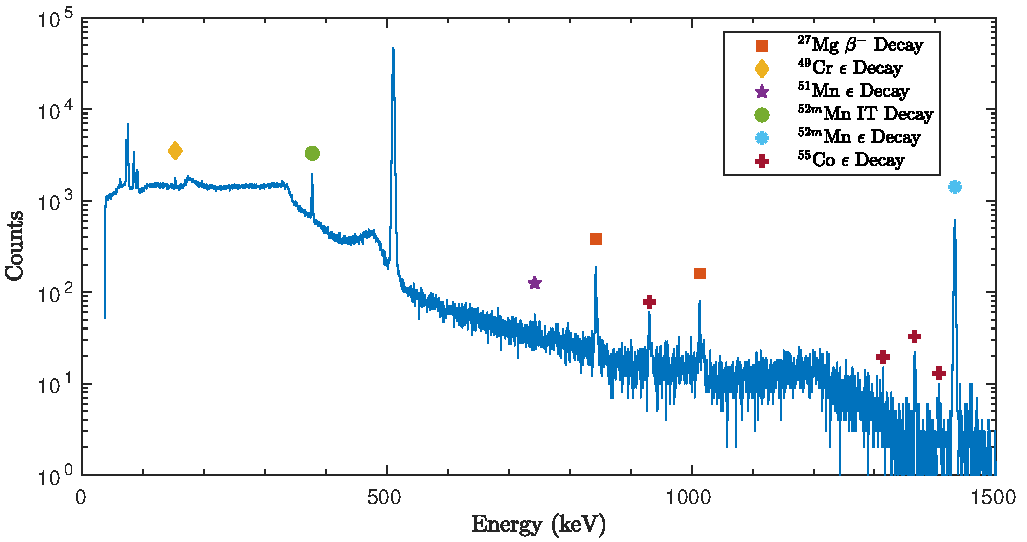
\includegraphics[width=0.75\textwidth]{./figures/sample_gspec_fe.pdf}
 % sample_gspec.pdf: 489x257 pixel, 72dpi, 17.25x9.07 cm, bb=0 0 489 257
 \caption{A gamma spectrum  from an activated Fe foil at approximately 55\,MeV (the maximum incident proton energy), collected 25 minutes after end-of-bombardment. Several observed reaction products are visible in this spectrum, and  the \ce{^{51}Cr} and \ce{^{52m}Mn} decay lines, which form two of the   primary reaction channels of interest, are  clearly isolated from surrounding peaks. }
 \label{fig:gspec_femn}
\end{figure*}

% Following  acquisition, the decaying product nuclei corresponding to each observed peak in the collected spectra were identified.
The net  counts in each fitted gamma-ray photopeak were converted into  activities for the decaying  activation products.
% , using calibrated detector efficiencies and gamma-ray intensities for each transition.
% and  corrections for gamma-ray attenuation within each foil packet
% The calibrated detector efficiencies, along with gamma-ray intensities for each transition and  corrections for gamma-ray attenuation within each foil packet, were used to convert the net  counts in each fitted gamma-ray photopeak into an activity for the decay of the activation products.  
% 
% Re-introduce this next line for the journal version
% 
% 
% The nuclear decay data used in this work is tabulated, for reference, in \autoref{tab:fe_nudat_table_monitors} and \autoref{tab:fe_nudat_table_nb} of Appendix \ref{sec:fe_data}.
The   half-lives and gamma-ray branching ratios  used for all calculations of measured cross sections reported in this work  have been taken from the most recent edition of  Nuclear Data Sheets for each  mass chain
\cite{Singh2015a,Chen2011a,Wu2000,Burrows2007,Burrows2006,Burrows2008,Wang2017,Dong2015,Dong2014,JUNDE2008787,Junde2011,Bhat1998,Nesaraja2010,Browne2013,Zuber20151,NICHOLS2012973,ERJUN2001,Singh2007}.
Corrections (typically \textless0.2\%) for gamma-ray attenuation within each foil packet were made, using  photon attenuation coefficients from the XCOM photon cross sections database\,\cite{berger2011xcom}.
% As nearly all of the product nuclei have multiple high-intensity gamma-rays, decay gamma-rays from the product nuclei were measured at multiple points in time (up to 2 weeks after EoB), as well as multiple independent activity measurements at each time point, based on each of its observed gamma-rays.
% Decay gamma-rays from the product nuclei were measured at multiple points in time (up to 2 weeks after EoB), and as nearly all of the product nuclei have multiple high-intensity gamma-rays, this provided independent activity measurements at each time point.
% activity for each gamma-ray possesses a 
EoB activities were determined by $\chi^2$-fitting of all observed decay gammas for a product to the decay curve.
The total  uncertainty in  activity is the propagated sum of the uncertainty in  fitted peak areas, uncertainty in detector efficiency calibration,  uncertainty in the gamma-ray branching ratio data, and uncertainty in photon attenuation coefficients (taken as~5\%).




As in our previous work, these activities were used to calculate 
% cross sections, and are differentiated between 
cumulative and independent cross sections\,\cite{Voyles2018a}.
% For the first observable product nuclide in a mass chain
For the first product nuclide in a mass chain with observable decay gammas, its (p,x) cross section is reported as a cumulative cross section ($\sigma_c$), which is the sum of direct production of that nucleus, as well as decay of its  precursors and any other independent cross sections leading to that nucleus. 
% In addition, 
Cumulative cross sections are reported whenever it is impossible to use decay spectrometry to distinguish independent production of a nucleus from decay feeding.
For all remaining observed reaction products in the mass chain, and cases where no decay precursors exist, independent cross sections  ($\sigma_i$) corresponding to a single 
% exit channel 
residual product are reported, 
% allowing for determination of the independent production via subtraction  and 
facilitating comparison to reaction model calculations.  
Solutions to the first- and higher-order  Bateman equations are used for separation of  feeding contributions from decay precursors, so that  independent cross sections may be reported\,\cite{bateman1910solution,Cetnar2006}.







% Since many of the reaction products populated by energetic protons are more than one decay off of stability, many of these are produced not only  directly by reactions, but also indirectly by decay down a mass chain.
% To this end, it is useful to differentiate between the types of cross sections reported in this work. 
% For the first observable product nuclei in a mass chain, its (p,x) cross section will be reported as a cumulative cross section ($\sigma_c$), which is the sum of direct production of that nucleus, as well as decay of its  precursors and any other independent cross sections leading to that nucleus. 
% % In addition, 
% Cumulative cross sections will be reported whenever it is impossible to use decay spectrometry to distinguish independent production of a nucleus from decay feeding.
% For all remaining observed reaction products in the mass chain, and cases where no decay precursors exist, independent cross sections ($\sigma_i$) will be reported, allowing for determination of the independent production via subtraction  and facilitating comparison to reaction model calculations.  
% 
% 
% 
% % To convert these activities into cross sections, c
% Corrections must be made for the decay of the various reaction products during the time between EoB and the spectrum acquisition, in order to calculate $A_0$, the initial activity at EoB, from the measured activities.
% The use of  multiple gamma-rays at multiple points after EoB to calculate initial activities  for each observed product nucleus allows for a more accurate  determination of $A_0$ than simply basing its calculation off of a single gamma-ray observation.
% For the case of cumulative cross sections, EoB activities were quantified by fitting the activities observed at multiple time points $t$ (since EoB) to the well-known radioactive decay law.
% % \begin{equation}
% % A\pp{t} = A_0 e^{-\lambda t}
% % \end{equation}
% Nonlinear regression was used for this fitting process, minimizing on $\chi^2$\,/\,degree of freedom, so that not only would the uncertainty-weighted EoB activities be fitted, but that a 1-$\sigma$ confidence interval in $A_0$ could be reported as as well.
% As with the gamma-ray intensities, all lifetimes used in this work are tabulated in \autoref{tab:fe_nudat_table_monitors} and \autoref{tab:fe_nudat_table_nb} of \ref{sec:fe_data}.
% In the case of independent cross sections, a similar process was followed, quantifying $A_i\pp{t=0} = A_{i,0}$, the EoB activity of nuclide $i$, by instead regressing to the solutions to the Bateman equation\,\cite{bateman1910solution,Cetnar2006}:
% \begin{equation}
% A_n\pp{t} = \lambda_n \sum_{i=1}^n \left[  N_{i,0} \times \pp{\prod_{j=i}^{n-1}\lambda_j} \times \pp{\sum_{j=i}^n \dfrac{e^{-\lambda_j t}}{\prod_{i\neq j}^n \pp{\lambda_i - \lambda_j}}  }   \right]
% \end{equation}
% where $j$ refers to a precursor nucleus populating a specific end-product.  
% While higher-order terms were added if needed, typically for an isomeric state in a particular mass chain,  the second-order expansion ($n=2$) was often sufficient to quantify EoB activities in a mass chain, simplifying to:
% \begin{equation}
% A_2\pp{t} = \dfrac{A_{1,0}\lambda_2}{\lambda_1 - \lambda_2} \pp{e^{-\lambda_2 t} - e^{-\lambda_1 t}} + A_{2,0} e^{-\lambda_2 t}
% \end{equation}
% In these cases, the previously-quantified EoB activities from decay precursors ($A_{1,0}$, etc) would be substituted in, so that the feeding contributions from decay could be separated and an independent cross section reported.
% After quantifying the cumulative EoB activities at the top of a mass chain and all subsequent independent EoB activities, these will be later used to report the various cross sections for all observed reaction products and isomeric states. 





% A citation in text uses the command \verb+\cite{#1}+ or
% \verb+\onlinecite{#1}+ and refers to an entry in the bibliography. 
% An entry in the bibliography is a reference to another document.

\subsection{\label{sec:dosimetry_fe}Proton fluence determination}


% In addition to 
% the stack's overall 
% measuring beam current  using  a current integrator, t
Thin \ce{^{nat}Ti} and \ce{^{nat}Cu} foils  
% included along with the \ce{^{nat}Fe} targets, 
% at each energy position, 
were co-irradiated to measure beam current at each position within the stack.
% These foils have been recommended for use as proton monitor foils in the 30 \textless\ E$_\text{p}$ \textless\ 100 MeV regime by the IAEA, as the
The IAEA-recommended \ce{^{nat}Ti}(p,x)\ce{^{46}Sc}, \ce{^{nat}Ti}(p,x)\ce{^{48}V},  \ce{^{nat}Cu}(p,x)\ce{^{62}Zn}, and \ce{^{nat}Cu}(p,x)\ce{^{63}Zn} monitor reactions were used 
% for  proton fluence measurement 
% , using values  
% and uncertainties 
% from the 2017 IAEA re-evaluation  
\cite{Hermanne2018}.
Systematically enhanced fluence from \ce{^{nat}Ti}(p,x)\ce{^{48}Sc} co-production was avoided by only using the 928.327, 944.130, and 2240.396\,keV decay gammas  from \ce{^{48}V}.
Using the formalism outlined in our previous work, the integral form of the well-known activation equation was used to  determine proton fluence ($I \Delta t $),
% in each monitor foil
in order to account for energy loss across each monitor foil \cite{Voyles2018a}.
% \begin{equation}
% I \Delta t = \dfrac{A_0 \Delta t}{\rho \Delta r \pp{1-e^{-\lambda \Delta t}} \int \sigma\pp{E} \dfrac{d\phi}{dE} dE}
% \end{equation}
The propagated uncertainty in proton fluence is calculated as the quadrature sum of (1) the uncertainty in quantified EoB activity, (2) uncertainty in the duration of irradiation (conservatively estimated at 10 s, to account for any transient changes in beam current), (3) uncertainty in foil areal density, (4) uncertainty in monitor product half-life (included, but normally negligible), (5) uncertainty in IAEA recommended cross section (using values  from the 2017 IAEA re-evaluation\,\cite{Hermanne2018}), and (6) uncertainty in differential proton fluence (from transport simulations).





% Because REV\TeX\ uses the \verb+natbib+ package of Patrick Daly, 
% the entire repertoire of commands in that package are available for your document;
% see the \verb+natbib+ documentation for further details. Please note that
% REV\TeX\ requires version 8.31a or later of \verb+natbib+.

\subsection{\label{sec:proton_transport_fe}Proton transport calculations}

Estimates of the proton beam energy for preliminary stack designs were calculated using the Anderson \& Ziegler (A\&Z) stopping power formalism\,\cite{Andersen_Ziegler_1977,Ziegler1985,Ziegler1999}.
However, the 
% more rigorous  
transport code FLUKA-2011.2x.3 was used for simulation of the full 3-D target stack and to determine the full proton energy and fluence distribution for each foil\,\cite{Bohlen2014a}. 
$10^8$ source protons were used for all FLUKA simulations, 
% which places the 
yielding a statistical uncertainty 
% in proton energy distributions at 
of less than 0.01\%.
As with the determination of proton fluence in the monitor foils, the progressively increasing energy straggle towards the rear of each stack is accounted for using 
% the differential proton fluence from 
FLUKA.
% simulation of proton transport.
These energy distributions $\frac{d\phi}{dE}$ were used to calculate a flux-weighted average proton  energy $\langle E \rangle$, which accounts for the slowing-down of protons within a foil (particularly in the low-energy stack) and reports the effective  energy centroid for each foil.
% \begin{equation}
% \langle E \rangle = \dfrac{{\displaystyle\int E \dfrac{d\phi}{dE} dE}}{{\displaystyle\int \dfrac{d\phi}{dE} dE}}
% \end{equation}
To report a complete description of the representative energy for each foil, a bin width is provided through the  energy uncertainty, calculated as the full width at half maximum (FWHM) of the FLUKA-modeled energy distribution for each foil.


% To correct for a spread in the apparent proton fluence, seen most strongly in rear stack positions, t
The \enquote{variance minimization} techniques utilized in our recent work and established by Graves \etal\ have been used to reduce uncertainty in proton fluence assignments due to poorly-characterized stopping power\,\cite{Voyles2018a,Graves2016}.
This method is based on the assumption that the independent measurements of proton fluence from the different monitor reactions 
% used in this work 
should all be consistent at each 
% energy 
position.
% Assuming that the recommended monitor reaction cross sections and FLUKA-modeled energy distributions are both accurate, 
% Any residual disagreement in the  observed proton fluences is  primarily due to poorly-characterized stopping power in simulations or a systematic error in the 
% % stack design, namely, the
% areal densities of the stack components. 
This disagreement is minor at the front of the stack, but gets progressively worse as the beam travels through the stack, due to the compounded effect of systematic uncertainties.
% in stack areal densities.



When performing  a variance minimization, it is important to apply this variation of effective areal density  to the stack components which  have the most significant impact on beam energy loss.
% degradation, as any systematic error in the areal densities used for these components will cause a disagreement in the observed fluences.
% For the 55\,MeV stack
Therefore, the aluminum degraders are used for variance minimization for the 55\,MeV stack, as they make up more than 80\% of the areal density of the stack.
% , and thus play the largest role in beam degradation.
For the 25\,MeV stack, the Kapton tape was chosen for variance minimization, as the foil packets themselves are responsible for the majority of beam degradation.
While it only makes up approximately 20\% of the low-energy stack's areal density, the Kapton surrounding each foil packet has a greater areal density than the foil itself.
In addition, it is far easier to directly characterize the areal density of the metallic foils than it is for the Kapton, resulting in only an approximate value for the latter.
% While it might seem obvious, t
The contributions to the slowing of the beam due to the adhesive have often been neglected in much work performed to date. 
This is of relatively minor consequence for higher-energy irradiations (especially relative to any beam degraders), but 
% the stopping power of the Kapton 
becomes increasingly important for proton energies below 
% approximately 
25\,MeV, causing as much as an additional loss of 8\,MeV  by the time it reaches the end of the stack.
% by the rear of this stack.
% , making the precise areal density a source of significant uncertainty.





In performing the  minimization, the areal density of each of the  aluminum degraders (for the 55\,MeV stack)  was varied uniformly in FLUKA simulations  by a factor of up to $\pm$25\% of nominal values, to find the effective density which minimized variance in the measured proton fluence at the lowest energy position (Ti-07, Cu-07).
For the 25\,MeV stack, the areal density reached in the minimization of the 55\,MeV stack was used for  the E-09 and H-01 aluminum degraders
% was taken from that reached in the minimization of the 55\,MeV stack.
% Using this value, 
and the areal density of each of the  Kapton tape  layers  was 
% likewise 
varied 
% uniformly   
by 
% a factor of up to 
$\pm$25\%, 
% of nominal values
to find the effective density which minimized variance in the measured proton fluence at the next-to-lowest energy position (Ti-19, Cu-19).
These 
% lowest energy 
positions were chosen as  minimization candidates as they are the most sensitive to systematic uncertainties in stack design.
% , due to the compounded effect of proton stopping powers.
In the 25\,MeV stack, activity was not seen in gamma spectrometry for the lowest-energy (Cu-20) monitor foil, implying that the beam was stopped at some point in between Ti-20 and Cu-20.
This observation 
% is conclusive proof 
indicates that  the true areal densities of the stack components differ from nominally measured values (primarily for the difficult-to-characterize Kapton tape), as transport calculations using nominal areal densities predict that the beam should exit the stack 
% (at the SS-6 profile monitor) 
with an energy of approximately 7\,MeV.
As a result, this position was not used for minimization, with the Ti-19 and Cu-19 position being the lowest-energy reliable monitor foils in the stack.
% % Remove these next two liens for the journal version
% % 
% With the exception of two foils (Cu-20 and Ti-20), each activated foil had a small \enquote{blister} under the Kapton tape layer, caused by a combination of thermal swelling and the formation of short-lived beta activities.
% % \comment{Maybe some Ne formed by Al(p,2a)Ne / Si(p,2ap)Ne?}
% This blister   verifies that the primary proton beam was incident upon the foil, and provided the first evidence (before gamma-ray spectrometry) that the beam was stopped in the stack between Fe-14 and Ti-20.
% 
% Re-introduce the rest of this paragraph for the journal version
% 
% 
The results of the minimization technique indicate a clear minimum in proton fluence variance for flux-weighted average 22.71\,MeV protons entering the last energy position of the 55\,MeV stack.
This is approximately 2\,MeV lower than the 
% nominal 
FLUKA simulations, and approximately 2\,MeV lower than 
% nominal 
A\&Z calculations, both of which used the nominal 2.80\,g/cm$^3$ measured density of the  aluminum degraders.
This energy corresponds to an aluminum areal density  4.43\% greater than 
% nominal 
measurements and 
% serves as a lump correction 
corrects for other minor systematic uncertainties in stack design.
% , including stack areal densities and incident beam energy.
Similarly, for the 25\,MeV stack, variance minimization converges on  flux-weighted average 9.23\,MeV protons entering the Fe-13/Ti-19/Cu-19 energy position, which is approximately 4\,MeV lower than the nominal FLUKA simulations, and approximately 5\,MeV lower than nominal A\&Z calculations.
This energy corresponds to a Kapton tape areal density of 5.69\% greater than nominal measurements, which is completely reasonable given the lack of areal density data from the manufacturer.
The impact of this variance minimization for improving disagreement in proton fluence is  clearly  seen in   \autoref{fig:fe_variance_mins}.




\begin{figure*}
    \centering
    \subfloat{
        \centering
        \hspace{-5pt}\subfigimg[width=0.485\textwidth]{a)}{./figures/before_minimization_plot.pdf}{50}
%         \caption{ Decay curve for the isomeric transition of \ce{^{115m}In}.}
         %         \refstepcounter{subfigure}
         \label{fig:fe_before_minimization}
   \hspace{-5pt}}%
     \subfloat{
        \centering

        \subfigimg[width=0.485\textwidth]{b)}{./figures/after_minimization_plot_alt.pdf}{50}
         %         \refstepcounter{subfigure}
         \label{fig:fe_after_minimization}
   \hspace{-5pt}}%
    \caption{Results of variance minimization through increasing the effective areal density of the  aluminum degraders by 4.43\% (55\,MeV stack) and Kapton tape by 5.69\% (25\,MeV stack). A noticeable reduction of variance in measured proton fluence is seen,  particularly at the  rear stack positions.  Open data points represent the 25\,MeV stack, and closed data points represent the 55\,MeV stack.} 
     \label{fig:fe_variance_mins}
\end{figure*}



% Re-introduce this paragraph for the journal version
% 
An enhanced version of the final \ce{^{nat}Ti}(p,x)\ce{^{46}Sc}, \ce{^{nat}Ti}(p,x)\ce{^{48}V}, \ce{^{nat}Cu}(p,x)\ce{^{62}Zn}, and \ce{^{nat}Cu}(p,x)\ce{^{63}Zn} monitor reaction fluences is shown in \autoref{fig:fe_fluence_plot}.
% Without the reliable use of the  \ce{^{nat}Al}(p,x)\ce{^{22}Na} and \ce{^{nat}Al}(p,x)\ce{^{24}Na} monitor channels, local interpolation cannot be used for fluence assignment to the Nb foils, and global interpolation is reliant upon a validated model for fluence loss.
The uncertainty-weighted mean  for the two \ce{^{nat}Cu}(p,x) and two \ce{^{nat}Ti}(p,x) monitor channels was calculated at each energy position, to determine the final fluence assignments for the Cu and Ti foils, respectively, and the uncertainty-weighted mean  for all four monitor channels was used to determine the final fluence assignments for the Fe foils.
Uncertainty in each final proton fluence  is  calculated by error propagation of the individual monitor channel fluence values  at each energy position.
These weighted-mean fluences are  plotted  in \autoref{fig:fe_fluence_plot}, along with the estimated fluence according to both  FLUKA transport 
and an uncertainty-weighted linear $\chi^2$ fit to the individual monitor channel fluence measurements.
Both models reproduce the observed fluence data consistently within uncertainty for the 55\,MeV stack, with the FLUKA model predicting a slightly greater fluence loss throughout the stack.
However, neither model is capable of accurately modeling the rapid decrease in apparent fluence at the rear of the 25\,MeV stack.   
These models are used purely to provide an extrapolation from the highest-energy position back to the \enquote{front} of each stack, to compare with the nominal fluence measured by  the beamline current integrators.
% 
% 
% 
% 
% 
% This involved minimizing on $\chi^2$ / degree of freedom, so that  a 95\% confidence interval in fluence would be reported as as well.
% As with the FWHM, a greater than 1$\sigma$ confidence interval is used for reporting fluence uncertainty to avoid an unrealistically small fluence confidence interval, based on the spread in observed fluence from Al and Cu monitor foils.
% The fluence and 2$\sigma$ uncertainties from this weighted-fit line are thus used in calculations of the various Nb(p,x) cross sections


% \begin{figure}
%  \centering
%  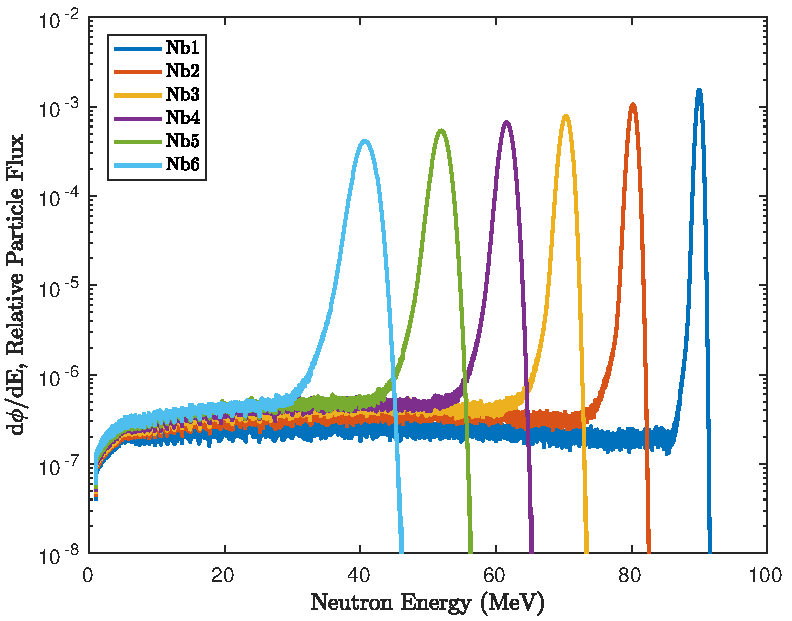
\includegraphics[width=0.5\linewidth]{./figures/Nb_ptallies.pdf}
%  % Nb_ptallies.pdf: 380x298 pixel, 72dpi, 13.41x10.51 cm, bb=0 0 380 298
%  \caption{Final variance minimized incident proton energy distributions for the Nb foils, as simulated in FLUKA. The distribution tallies in each foil are all normalized to be per source proton, which was $10^8$ in all simulations. As the beam is degraded, proton energy distributions become visibly broadened due to straggling, and drop in magnitude due to scattering losses.}
%  \label{fig:Nb_ptallies}
% \end{figure}

\begin{figure}
 \centering
 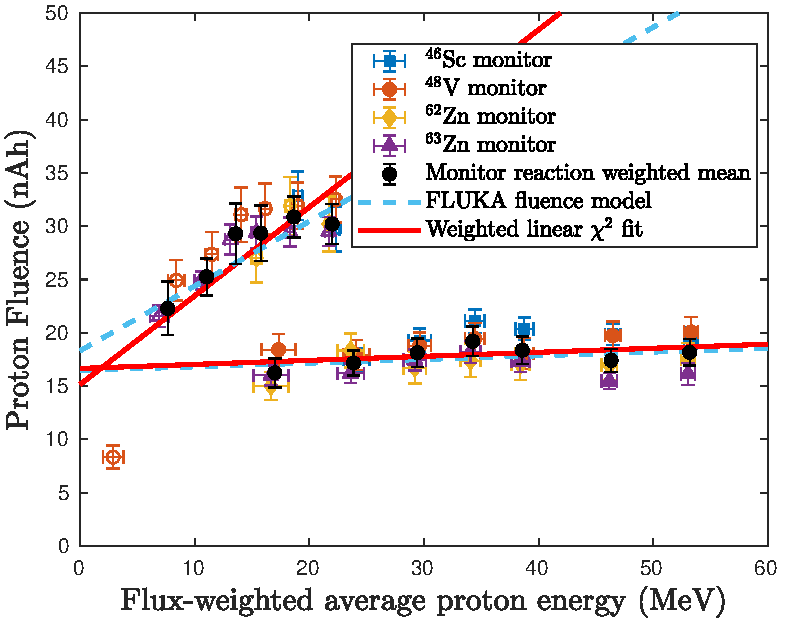
\includegraphics[width=0.495\textwidth]{./figures/fluence_plot.pdf}
 % Nb_ptallies.pdf: 380x298 pixel, 72dpi, 13.41x10.51 cm, bb=0 0 380 298
 \caption{Final uncertainty-weighted mean proton fluences throughout the target stack, based on the variance-minimized observed fluence from the the  \ce{^{nat}Ti}(p,x)\ce{^{46}Sc}, \ce{^{nat}Ti}(p,x)\ce{^{48}V}, \ce{^{nat}Cu}(p,x)\ce{^{62}Zn}, and \ce{^{nat}Cu}(p,x)\ce{^{63}Zn} monitor reactions. Open data points represent the 25\,MeV stack, and closed data points represent the 55\,MeV stack.} 
%  A 95\% ($2\sigma$) confidence interval is reported in the fitted proton fluence, to ensure a realistic uncertainty in fluence, which encompasses the true absolute fluence. 
%   A clear loss of 
%   The fluence  drops by approximately \textred{7.2--8.9\%} from the incident fluence of \textred{196.9--198.8 nAh} over the length of each target stack, based on fluence loss models from FLUKA simulations and an empirical fit to  fluence measurements.}  
%   This is due to a combination of beam utilization, as well as scattering.}
 \label{fig:fe_fluence_plot}
\end{figure}






\subsection{\label{sec:calcs_sec_fe}Calculation of measured cross sections}


Using the quantified EoB activities along with the variance-minimized proton fluence, it is possible to calculate 
% the final 
cross sections for 
% the various 
observed (p,x) reactions.
While thin ($\approx$ 10--20\,mg/cm$^2$)  foils were irradiated to minimize the energy bins of these cross section measurements, 
% it is important to note that 
all cross sections reported here are flux-averaged  
% cross sections, 
over the energy distribution subtended by each foil.
% Re-introduce this next line for the journal version
% , as seen in \autoref{fig:Fe_ptallies}.
% For both the cumulative and independent activities quantified, cross sections were calculated using the formalism outlined in our previous work \cite{Voyles2018a}.
% as:
% \begin{equation}
% \sigma = \dfrac{A_0 }{\rho \Delta r I \pp{1-e^{-\lambda \Delta t}} }
% \end{equation}
% where $A_0$ is the EoB activity for the  reaction product, $I$ is the proton current, $\rho \Delta r$ is the foil's areal density, $\lambda$ is the monitor reaction product's decay constant, and $\Delta t$ is the length of irradiation.
The beam current, measured using a current integrator connected to the electrically-isolated target box, remained stable for the duration of the irradiation.
The propagated uncertainty in cross section is calculated as the quadrature sum of the uncertainty in quantified EoB activity (which includes uncertainty in detector efficiencies), uncertainty in the duration of irradiation (conservatively estimated at 10\,s, to account for any minor transient changes in beam current), uncertainty in foil areal density, uncertainty in monitor product half-life (included, but normally negligible),  and uncertainty in proton current (quantified by error propagation of the monitor reaction fluence values  at each energy position).
% , as seen in \autoref{fig:fe_fluence_plot}).


% \begin{figure}
%  \centering
%  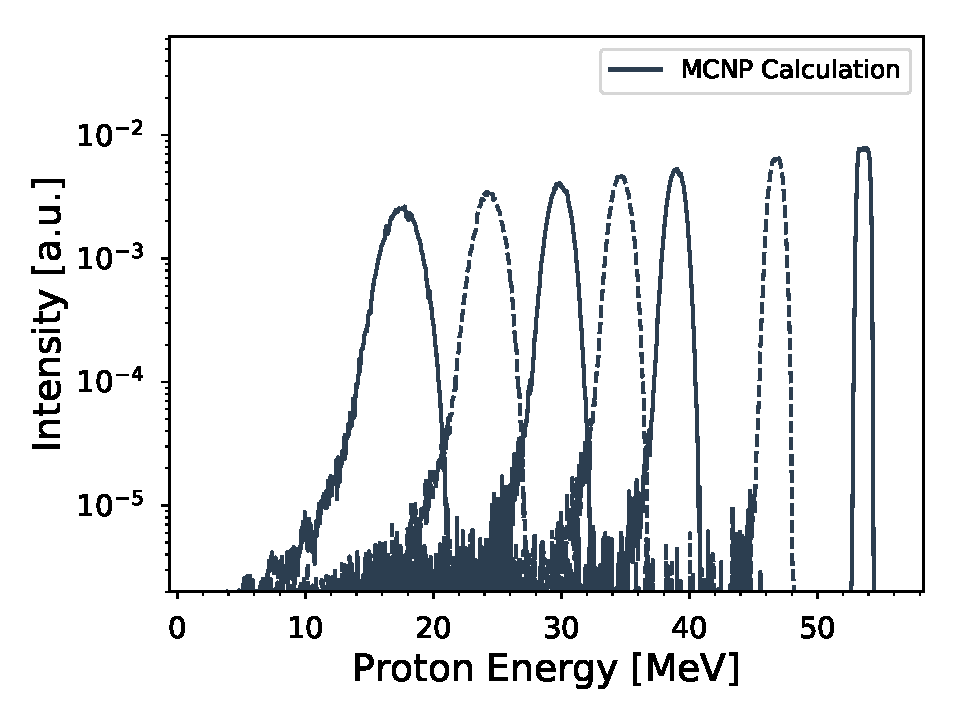
\includegraphics[width=0.5\linewidth]{./figures/Fe_mcnp_spectrum.pdf}
%  % Nb_ptallies.pdf: 380x298 pixel, 72dpi, 13.41x10.51 cm, bb=0 0 380 298
%  \caption{\textred{Add 25\,MeV stack tallies here! } Final variance minimized incident proton energy distributions for the Fe foils, as simulated in FLUKA. The distribution tallies in each foil are all normalized to be per source proton, which was $10^8$ in all simulations. As the beam is degraded, proton energy distributions become visibly broadened due to straggling, and drop in magnitude due to scattering losses.}
%  \label{fig:Fe_ptallies}
% \end{figure}


\section{\label{sec:results_fe}Results and Discussion}


\subsection{Measurement of nuclear excitation functions}

After irradiation, all foils were 
% confirmed to 
still sealed in their Kapton packets, verifying that no activation products were lost due to packet failure.
% and dispersal.
With the exception of a single foil (Cu-20, in the 25\,MeV stack), each activated foil had a small \enquote{blister} under the Kapton tape layer, caused by a combination of 
% thermal swelling, 
off-gassing of oxides and the formation of gaseous short-lived beta activities in the tape.
% \comment{Maybe some Ne formed by Al(p,2a)Ne / Si(p,2ap)Ne?}
This blister   verifies that the primary proton beam was incident upon the foil, and provides additional 
% the first 
evidence 
% (before gamma-ray spectrometry) 
that the beam was stopped in the stack between Ti-20 and Cu-20.
% , producing a Bragg peak at this location.  
Using the \ce{^{nat}Ti}(p,x)\ce{^{46}Sc}, \ce{^{nat}Ti}(p,x)\ce{^{48}V}, \ce{^{nat}Cu}(p,x)\ce{^{62}Zn}, and \ce{^{nat}Cu}(p,x)\ce{^{63}Zn} monitor reactions, as discussed in \autoref{sec:proton_transport_fe}, a fluence of 17.9$~\pm~$1.0\,nAh 
% 18.8$\pm$1.0\,nAh
was calculated to be incident upon the 55\,MeV target stack using the FLUKA fluence model, and a  fluence of 19.0$~\pm~$1.3\,nAh using the linear fit model.
Similarly, for the 25\,MeV stack, a fluence of 27.5$~\pm~$8.3\,nAh 
% 33.2$\pm$4.7\,nAh
was calculated to be incident upon the 
% 55\,MeV 
target stack using the FLUKA fluence model, and a  fluence of 31.7$~\pm~$3.7\,nAh using the linear fit model to the four frontmost compartments (before the fluence loss becomes strongly nonlinear).
% 37.0$\pm$9.3\,nAh using the linear fit model.
% All of these 
Both linear models are consistent with the nominal fluence of 20.78\,nAh (for the 55\,MeV stack) and 31.61\,nAh (for the 25\,MeV stack) measured using the 
% beamline 
current integrators.
However, for both target stacks, the FLUKA transport model predicts a significant increase in proton fluence, in particular for the 25\,MeV stack.
This model fails to reproduce the fluence loss seen in monitor foils, and predicts a significantly higher production of lower-energy secondary protons not seen in the activation data.
As fluence loss scales with $\sigma_{\mathrm{tot}}\rho\Delta r$, it is expected that an extrapolation back to the stack entrance (through the SS-3/SS-5 profile monitors) will underestimate the nominal fluence incident upon the box.
This incident fluence dropped by approximately 
% 9.5\% to  17.0$\pm$2.4\,nAh (and by 
8.9\% to  17.3$~\pm~$1.5\,nAh using the linear fit model over the length of the 55\,MeV stack, which is consistent with similar measurements at the Los Alamos National Laboratory's Isotope Production Facility in the past\,\cite{Voyles2018a,Graves2016}.
This loss of fluence is due to a combination of 
% beam utilization for the various 
(p,x) reactions throughout the target stack, as well as large-angle deflections (primarily in the aluminum degraders) from scattering of the beam.




Using the final proton fluence at each energy position, cross sections for \ce{^{48,49,51}Cr}, \ce{^{48}V},  \ce{^{51,52m,52g,52,54,56}Mn},   \ce{^{52}Fe}, and \ce{^{55,56,57,58m,58g,58}Co}
 were extracted for (p,x) reactions  on \ce{^{nat}Fe} foils up to 55\,MeV, presented in \autoref{tab:fe_rp_table}.
For  (p,x) reactions on \ce{^{nat}Cu}, the (p,x) cross sections for  \ce{^{54}Mn}, \ce{^{57}Ni}, \ce{^{57,60,61}Co},   and \ce{^{60,61,64}Cu}  were extracted, 
% as recorded 
presented in \autoref{tab:cufe_rp_table}.
For  (p,x) reactions on \ce{^{nat}Ti}, the (p,x) cross sections for  \ce{^{43}K} and \ce{^{44g,44m,44,47,48}Sc}  were extracted, 
% as recorded 
presented in \autoref{tab:ti_rp_table}.
In addition, as there exist a number of isomers with radioactive ground states in these mass regions,  independent measurements of isomer-to-ground-state branching ratios for \ce{^{nat}Fe}(p,x)\ce{^{52m/g}Mn}, \ce{^{nat}Fe}(p,x)\ce{^{58m/g}Co}, and \ce{^{nat}Ti}(p,x)\ce{^{44m/g}Sc} were  extracted and are presented in \autoref{tab:fe_ibr_table}.
Comparisons  of the measured cross sections and isomer branching ratios with literature data (retrieved from EXFOR\,\cite{Otuka2014272}) are seen in the figures of 
% Appendices 
\ref{sec:fe_xs_figures} and \ref{sec:fe_ibr_figures}.
The propagated uncertainty in these cross sections varies widely based on the reaction product in question, with the major components  arising from uncertainty in EoB activity ($\pm$3--10\%), proton fluence ($\pm$5--13\%), and foil areal density ($\pm$0.1--0.3\%).



% % Please add the following required packages to your document preamble:
% % \usepackage{booktabs}
% \begin{table}
% \centering
% \caption{Measured cross sections for the various \ce{^{nat}Fe}(p,x) reaction products observed in this work. Cumulative cross sections are designated as $\sigma_c$, independent cross sections are designated as $\sigma_i$. Uncertainties are reported in the least significant digit.}
% \label{tab:fe_rp_table}
% \small
% \resizebox{\textwidth}{!}{%
% % \begin{tabular}{@{}lllllllllllllll@{}}
% \begin{tabular}{@{}ccccccccccccccc@{}}
% \toprule\toprule
%                             & \multicolumn{14}{c}{Production cross section (mb)}                                                                                                         \\ \cmidrule(l){2-15} 
% % E$_\text{p}$ (MeV)          & $89.74^{+0.48}_{-0.43}$ & $79.95^{+0.67}_{-0.64}$ & $70.17^{+0.91}_{-0.85}$ & $61.58^{+1.03}_{-0.98}$ & $52.10^{+1.25}_{-1.20}$ & $41.05^{+1.62}_{-1.54}$ \\ \midrule
% % E$_\text{p}$ (MeV)  & $53.45 \pm0.61$ & $46.63 \pm0.68$ & $38.93 \pm0.78$ & $34.62 \pm0.85$ & $29.84 \pm0.96$ & $24.4 \pm1.1$ & $22.71 \pm0.43$ & $19.36 \pm0.56$ & $17.6 \pm1.5$ & $16.54 \pm0.48$ & $14.52 \pm0.49$ & $12.11 \pm0.53$ & $9.23 \pm0.61$ & $4.10 \pm0.73$\\  \midrule
% E$_\text{p}$ (MeV)&	\makecell{53.45\\$\pm$0.61} &	\makecell{46.63\\$\pm$0.68} &	\makecell{38.93\\$\pm$0.78} &	\makecell{34.62\\$\pm$0.85} &	\makecell{29.84\\$\pm$0.96} &	\makecell{24.4\\$\pm$1.1} &	\makecell{22.71\\$\pm$0.43} &	\makecell{19.36\\$\pm$0.56} &	\makecell{17.6\\$\pm$1.5} &	\makecell{16.54\\$\pm$0.48} &	\makecell{14.52\\$\pm$0.49} &	\makecell{12.11\\$\pm$0.53} &	\makecell{9.23\\$\pm$0.61} &	\makecell{4.10\\$\pm$0.73}\\  \midrule
% \ce{^{48}Cr}\,($\sigma_c$)&	\makecell{0.172\\$\pm$0.011} &	\makecell{0.01376\\$\pm$0.00080} &	\makecell{0.00435\\$\pm$0.00029} &	-- &	-- &	-- &	-- &	-- &	-- &	-- &	-- &	-- &	-- &	--\\
% \ce{^{48}V}\,($\sigma_i$)&	\makecell{6.38\\$\pm$0.43} &	\makecell{4.64\\$\pm$0.29} &	\makecell{0.513\\$\pm$0.035} &	\makecell{0.1096\\$\pm$0.0080} &	-- &	-- &	-- &	-- &	-- &	-- &	-- &	-- &	-- &	--\\
% \ce{^{48}V}\,($\sigma_c$)&	\makecell{6.55\\$\pm$0.43} &	\makecell{4.65\\$\pm$0.29} &	\makecell{0.517\\$\pm$0.035} &	\makecell{0.1096\\$\pm$0.0080} &	-- &	-- &	-- &	-- &	-- &	-- &	-- &	-- &	-- &	--\\
% \ce{^{49}Cr}\,($\sigma_c$)&	\makecell{1.83\\$\pm$0.12} &	\makecell{2.25\\$\pm$0.18} &	\makecell{1.20\\$\pm$0.11} &	\makecell{0.315\\$\pm$0.036} &	-- &	-- &	-- &	-- &	-- &	-- &	-- &	-- &	-- &	--\\
% \ce{^{51}Mn}\,($\sigma_c$)&	\makecell{11.77\\$\pm$0.74} &	\makecell{15.69\\$\pm$0.94} &	\makecell{11.78\\$\pm$0.77} &	\makecell{6.15\\$\pm$0.41} &	\makecell{0.475\\$\pm$0.039} &	\makecell{0.679\\$\pm$0.047} &	\makecell{1.060\\$\pm$0.063} &	\makecell{1.97\\$\pm$0.15} &	\makecell{2.10\\$\pm$0.17} &	\makecell{1.98\\$\pm$0.19} &	\makecell{1.46\\$\pm$0.13} &	\makecell{0.584\\$\pm$0.041} &	-- &	--\\
% \ce{^{51}Cr}\,($\sigma_i$)&	\makecell{65.9\\$\pm$5.8} &	\makecell{81.0\\$\pm$5.9} &	\makecell{56.5\\$\pm$4.5} &	\makecell{27.6\\$\pm$2.3} &	\makecell{3.83\\$\pm$0.35} &	\makecell{0.90\\$\pm$0.12} &	\makecell{0.70\\$\pm$0.13} &	\makecell{0.150\\$\pm$0.049} &	\makecell{0.110\\$\pm$0.024} &	-- &	-- &	-- &	-- &	--\\
% \ce{^{51}Cr}\,($\sigma_c$)&	\makecell{77.6\\$\pm$5.7} &	\makecell{96.7\\$\pm$5.8} &	\makecell{68.3\\$\pm$4.4} &	\makecell{33.7\\$\pm$2.3} &	\makecell{4.30\\$\pm$0.35} &	\makecell{1.58\\$\pm$0.11} &	\makecell{1.76\\$\pm$0.11} &	\makecell{2.12\\$\pm$0.13} &	\makecell{2.21\\$\pm$0.17} &	\makecell{1.98\\$\pm$0.19} &	\makecell{1.46\\$\pm$0.13} &	\makecell{0.584\\$\pm$0.041} &	-- &	--\\
% \ce{^{52}Fe}\,($\sigma_c$)&	\makecell{2.74\\$\pm$0.17} &	\makecell{1.82\\$\pm$0.11} &	\makecell{1.60\\$\pm$0.10} &	\makecell{2.25\\$\pm$0.15} &	\makecell{0.770\\$\pm$0.052} &	\makecell{0.206\\$\pm$0.015} &	\makecell{0.192\\$\pm$0.013} &	\makecell{0.01297\\$\pm$0.00075} &	\makecell{0.00242\\$\pm$0.00021} &	-- &	-- &	-- &	-- &	--\\
% \ce{^{52m}Mn}\,($\sigma_i$)&	\makecell{8.29\\$\pm$0.52} &	\makecell{9.49\\$\pm$0.54} &	\makecell{13.69\\$\pm$0.88} &	\makecell{17.9\\$\pm$1.2} &	\makecell{23.3\\$\pm$1.5} &	\makecell{11.82\\$\pm$0.74} &	\makecell{5.78\\$\pm$0.33} &	\makecell{0.0763\\$\pm$0.0044} &	\makecell{0.0763\\$\pm$0.0057} &	\makecell{0.0754\\$\pm$0.0061} &	\makecell{0.0585\\$\pm$0.0052} &	-- &	-- &	--\\
% \ce{^{52g}Mn}\,($\sigma_i$)&	\makecell{11.58\\$\pm$0.72} &	\makecell{13.46\\$\pm$0.76} &	\makecell{20.8\\$\pm$1.3} &	\makecell{28.2\\$\pm$1.8} &	\makecell{21.8\\$\pm$1.5} &	\makecell{16.3\\$\pm$1.0} &	\makecell{10.37\\$\pm$0.64} &	\makecell{0.300\\$\pm$0.017} &	\makecell{0.1124\\$\pm$0.0085} &	\makecell{0.0428\\$\pm$0.0038} &	\makecell{0.00540\\$\pm$0.00050} &	-- &	-- &	--\\
% \ce{^{52}Mn}\,($\sigma_c$)&	\makecell{13.66\\$\pm$0.90} &	\makecell{15.6\\$\pm$1.1} &	\makecell{23.0\\$\pm$1.8} &	\makecell{30.9\\$\pm$2.1} &	\makecell{31.7\\$\pm$2.2} &	\makecell{18.5\\$\pm$1.3} &	\makecell{10.57\\$\pm$0.62} &	\makecell{0.313\\$\pm$0.019} &	\makecell{0.0393\\$\pm$0.0045} &	\makecell{0.0556\\$\pm$0.0048} &	\makecell{0.0185\\$\pm$0.0019} &	-- &	-- &	--\\
% \ce{^{54}Mn}\,($\sigma_i$)&	\makecell{131.0\\$\pm$8.5} &	\makecell{162\\$\pm$10} &	\makecell{167\\$\pm$12} &	\makecell{129\\$\pm$10} &	\makecell{42.2\\$\pm$3.4} &	\makecell{2.46\\$\pm$0.25} &	\makecell{1.10\\$\pm$0.13} &	\makecell{1.09\\$\pm$0.14} &	\makecell{1.47\\$\pm$0.17} &	\makecell{1.53\\$\pm$0.16} &	\makecell{1.36\\$\pm$0.12} &	\makecell{1.133\\$\pm$0.080} &	\makecell{0.747\\$\pm$0.075} &	\makecell{0.0600\\$\pm$0.0080}\\
% \ce{^{55}Co}\,($\sigma_i$)&	\makecell{9.43\\$\pm$0.63} &	\makecell{12.5\\$\pm$1.0} &	\makecell{15.7\\$\pm$1.2} &	\makecell{21.5\\$\pm$1.5} &	\makecell{48.4\\$\pm$3.6} &	\makecell{64.7\\$\pm$5.6} &	\makecell{61.0\\$\pm$4.5} &	\makecell{43.6\\$\pm$3.0} &	\makecell{33.6\\$\pm$3.4} &	\makecell{13.4\\$\pm$1.2} &	\makecell{0.377\\$\pm$0.035} &	\makecell{0.0421\\$\pm$0.0029} &	-- &	--\\
% \ce{^{56}Mn}\,($\sigma_c$)&	-- &	\makecell{0.518\\$\pm$0.039} &	\makecell{0.610\\$\pm$0.044} &	\makecell{0.462\\$\pm$0.045} &	\makecell{0.506\\$\pm$0.054} &	\makecell{0.405\\$\pm$0.033} &	\makecell{0.223\\$\pm$0.013} &	\makecell{0.0962\\$\pm$0.0056} &	\makecell{0.0329\\$\pm$0.0043} &	\makecell{0.0253\\$\pm$0.0021} &	\makecell{0.0132\\$\pm$0.0014} &	-- &	-- &	--\\
% \ce{^{56}Co}\,($\sigma_i$)&	\makecell{13.0\\$\pm$1.1} &	\makecell{16.3\\$\pm$1.4} &	\makecell{18.9\\$\pm$1.6} &	\makecell{23.6\\$\pm$1.7} &	\makecell{29.2\\$\pm$2.6} &	\makecell{47.8\\$\pm$3.2} &	\makecell{51.6\\$\pm$3.0} &	\makecell{82.6\\$\pm$5.0} &	\makecell{176\\$\pm$13} &	\makecell{197\\$\pm$16} &	\makecell{344\\$\pm$30} &	\makecell{376\\$\pm$24} &	\makecell{288\\$\pm$29} &	\makecell{3.54\\$\pm$0.47}\\
% \ce{^{57}Co}\,($\sigma_i$)&	-- &	\makecell{0.476\\$\pm$0.047} &	\makecell{0.539\\$\pm$0.060} &	\makecell{0.648\\$\pm$0.044} &	\makecell{1.170\\$\pm$0.090} &	\makecell{1.84\\$\pm$0.12} &	\makecell{2.36\\$\pm$0.14} &	\makecell{2.50\\$\pm$0.16} &	\makecell{3.20\\$\pm$0.25} &	\makecell{3.40\\$\pm$0.28} &	\makecell{5.14\\$\pm$0.47} &	\makecell{8.18\\$\pm$0.52} &	\makecell{11.5\\$\pm$1.2} &	\makecell{5.49\\$\pm$0.73}\\
% \ce{^{58m}Co}\,($\sigma_i$)&	-- &	-- &	-- &	\makecell{0.0427\\$\pm$0.0028} &	\makecell{0.0619\\$\pm$0.0042} &	\makecell{0.1054\\$\pm$0.0069} &	\makecell{0.172\\$\pm$0.011} &	\makecell{0.236\\$\pm$0.015} &	\makecell{0.241\\$\pm$0.019} &	\makecell{0.300\\$\pm$0.028} &	\makecell{0.475\\$\pm$0.044} &	\makecell{0.545\\$\pm$0.035} &	\makecell{0.477\\$\pm$0.049} &	\makecell{0.170\\$\pm$0.025}\\
% \ce{^{58g}Co}\,($\sigma_i$)&	-- &	-- &	-- &	\makecell{0.0884\\$\pm$0.0066} &	\makecell{0.0980\\$\pm$0.0074} &	\makecell{0.1118\\$\pm$0.0082} &	\makecell{0.1229\\$\pm$0.0084} &	\makecell{0.1484\\$\pm$0.0090} &	\makecell{0.333\\$\pm$0.028} &	\makecell{0.318\\$\pm$0.027} &	\makecell{0.919\\$\pm$0.090} &	\makecell{1.276\\$\pm$0.096} &	\makecell{1.56\\$\pm$0.17} &	\makecell{0.623\\$\pm$0.083}\\
% \ce{^{58}Co}\,($\sigma_i$)&	-- &	-- &	-- &	\makecell{0.1311\\$\pm$0.0072} &	\makecell{0.1599\\$\pm$0.0086} &	\makecell{0.217\\$\pm$0.011} &	\makecell{0.295\\$\pm$0.014} &	\makecell{0.384\\$\pm$0.018} &	\makecell{0.574\\$\pm$0.034} &	\makecell{0.618\\$\pm$0.039} &	\makecell{1.39\\$\pm$0.10} &	\makecell{1.82\\$\pm$0.10} &	\makecell{2.04\\$\pm$0.18} &	\makecell{0.792\\$\pm$0.086}\\ \bottomrule\bottomrule
% \end{tabular}
% }
% \end{table}
% Please add the following required packages to your document preamble:
% \usepackage{booktabs}
\begin{table}
\centering
\caption{Measured cross sections for the various \ce{^{nat}Fe}(p,x) reaction products observed in this work. Cumulative cross sections are designated as $\sigma_c$, independent cross sections are designated as $\sigma_i$.}
% Uncertainties are reported in the least significant digit.}
\label{tab:fe_rp_table}
\small
\resizebox{\textwidth}{!}{%
% \begin{tabular}{@{}lllllllllllllll@{}}
\begin{tabular}{@{}ccccccccccccccc@{}}
\toprule\toprule
                            & \multicolumn{14}{c}{Production cross section (mb)}                                                                                                         \\ \cmidrule(l){2-15} 
% E$_\text{p}$ (MeV)          & $89.74^{+0.48}_{-0.43}$ & $79.95^{+0.67}_{-0.64}$ & $70.17^{+0.91}_{-0.85}$ & $61.58^{+1.03}_{-0.98}$ & $52.10^{+1.25}_{-1.20}$ & $41.05^{+1.62}_{-1.54}$ \\ \midrule
% E$_\text{p}$ (MeV)  & $53.45 \pm0.61$ & $46.63 \pm0.68$ & $38.93 \pm0.78$ & $34.62 \pm0.85$ & $29.84 \pm0.96$ & $24.4 \pm1.1$ & $22.71 \pm0.43$ & $19.36 \pm0.56$ & $17.6 \pm1.5$ & $16.54 \pm0.48$ & $14.52 \pm0.49$ & $12.11 \pm0.53$ & $9.23 \pm0.61$ & $4.10 \pm0.73$\\  \midrule
E$_\text{p}$ (MeV)&	\makecell{53.45(61)} &	\makecell{46.63(68)} &	\makecell{38.93(78)} &	\makecell{34.62(85)} &	\makecell{29.84(96)} &	\makecell{24.4(11)} &	\makecell{22.71(43)} &	\makecell{19.36(56)} &	\makecell{17.6(15)} &	\makecell{16.54(48)} &	\makecell{14.52(49)} &	\makecell{12.11(53)} &	\makecell{9.23(61)} &	\makecell{4.10(73)}\\  \midrule
\ce{^{48}Cr}\,($\sigma_c$)&	\makecell{0.172(11)} &	\makecell{0.01376(80)} &	\makecell{0.00435(29)} &	-- &	-- &	-- &	-- &	-- &	-- &	-- &	-- &	-- &	-- &	--\\
\ce{^{48}V}\,($\sigma_i$)&	\makecell{6.38(43)} &	\makecell{4.64(29)} &	\makecell{0.513(35)} &	\makecell{0.1096(80)} &	-- &	-- &	-- &	-- &	-- &	-- &	-- &	-- &	-- &	--\\
\ce{^{48}V}\,($\sigma_c$)&	\makecell{6.55(43)} &	\makecell{4.65(29)} &	\makecell{0.517(35)} &	\makecell{0.1096(80)} &	-- &	-- &	-- &	-- &	-- &	-- &	-- &	-- &	-- &	--\\
\ce{^{49}Cr}\,($\sigma_c$)&	\makecell{1.83(12)} &	\makecell{2.25(18)} &	\makecell{1.20(11)} &	\makecell{0.315(36)} &	-- &	-- &	-- &	-- &	-- &	-- &	-- &	-- &	-- &	--\\
\ce{^{51}Mn}\,($\sigma_c$)&	\makecell{11.77(74)} &	\makecell{15.69(94)} &	\makecell{11.78(77)} &	\makecell{6.15(41)} &	\makecell{0.475(39)} &	\makecell{0.679(47)} &	\makecell{1.060(63)} &	\makecell{1.97(15)} &	\makecell{2.10(17)} &	\makecell{1.98(19)} &	\makecell{1.46(13)} &	\makecell{0.584(41)} &	-- &	--\\
\ce{^{51}Cr}\,($\sigma_i$)&	\makecell{65.9(58)} &	\makecell{81.0(59)} &	\makecell{56.5(45)} &	\makecell{27.6(23)} &	\makecell{3.83(35)} &	\makecell{0.90(12)} &	\makecell{0.70(13)} &	\makecell{0.150(49)} &	\makecell{0.110(24)} &	-- &	-- &	-- &	-- &	--\\
\ce{^{51}Cr}\,($\sigma_c$)&	\makecell{77.6(57)} &	\makecell{96.7(58)} &	\makecell{68.3(44)} &	\makecell{33.7(23)} &	\makecell{4.30(35)} &	\makecell{1.58(11)} &	\makecell{1.76(11)} &	\makecell{2.12(13)} &	\makecell{2.21(17)} &	\makecell{1.98(19)} &	\makecell{1.46(13)} &	\makecell{0.584(41)} &	-- &	--\\
\ce{^{52}Fe}\,($\sigma_c$)&	\makecell{2.74(17)} &	\makecell{1.82(11)} &	\makecell{1.60(10)} &	\makecell{2.25(15)} &	\makecell{0.770(52)} &	\makecell{0.206(15)} &	\makecell{0.192(13)} &	\makecell{0.01297(75)} &	\makecell{0.00242(21)} &	-- &	-- &	-- &	-- &	--\\
\ce{^{52m}Mn}\,($\sigma_i$)&	\makecell{8.29(52)} &	\makecell{9.49(54)} &	\makecell{13.69(88)} &	\makecell{17.9(12)} &	\makecell{23.3(15)} &	\makecell{11.82(74)} &	\makecell{5.78(33)} &	\makecell{0.0763(44)} &	\makecell{0.0763(57)} &	\makecell{0.0754(61)} &	\makecell{0.0585(52)} &	-- &	-- &	--\\
\ce{^{52g}Mn}\,($\sigma_i$)&	\makecell{11.58(72)} &	\makecell{13.46(76)} &	\makecell{20.8(13)} &	\makecell{28.2(18)} &	\makecell{21.8(15)} &	\makecell{16.3(10)} &	\makecell{10.37(64)} &	\makecell{0.300(17)} &	\makecell{0.1124(85)} &	\makecell{0.0428(38)} &	\makecell{0.00540(50)} &	-- &	-- &	--\\
\ce{^{52g}Mn}\,($\sigma_c$)&	\makecell{13.66(90)} &	\makecell{15.6(11)} &	\makecell{23.0(18)} &	\makecell{30.9(21)} &	\makecell{31.7(22)} &	\makecell{18.5(13)} &	\makecell{10.57(62)} &	\makecell{0.313(19)} &	\makecell{0.0393(45)} &	\makecell{0.0556(48)} &	\makecell{0.0185(19)} &	-- &	-- &	--\\
\ce{^{54}Mn}\,($\sigma_i$)&	\makecell{131.0(85)} &	\makecell{162(10)} &	\makecell{167(12)} &	\makecell{129(10)} &	\makecell{42.2(34)} &	\makecell{2.46(25)} &	\makecell{1.10(13)} &	\makecell{1.09(14)} &	\makecell{1.47(17)} &	\makecell{1.53(16)} &	\makecell{1.36(12)} &	\makecell{1.133(80)} &	\makecell{0.747(75)} &	\makecell{0.0600(80)}\\
\ce{^{55}Co}\,($\sigma_i$)&	\makecell{9.43(63)} &	\makecell{12.5(10)} &	\makecell{15.7(12)} &	\makecell{21.5(15)} &	\makecell{48.4(36)} &	\makecell{64.7(56)} &	\makecell{61.0(45)} &	\makecell{43.6(30)} &	\makecell{33.6(34)} &	\makecell{13.4(12)} &	\makecell{0.377(35)} &	\makecell{0.0421(29)} &	-- &	--\\
\ce{^{56}Mn}\,($\sigma_c$)&	-- &	\makecell{0.518(39)} &	\makecell{0.610(44)} &	\makecell{0.462(45)} &	\makecell{0.506(54)} &	\makecell{0.405(33)} &	\makecell{0.223(13)} &	\makecell{0.0962(56)} &	\makecell{0.0329(43)} &	\makecell{0.0253(21)} &	\makecell{0.0132(14)} &	-- &	-- &	--\\
\ce{^{56}Co}\,($\sigma_i$)&	\makecell{13.0(11)} &	\makecell{16.3(14)} &	\makecell{18.9(16)} &	\makecell{23.6(17)} &	\makecell{29.2(26)} &	\makecell{47.8(32)} &	\makecell{51.6(30)} &	\makecell{82.6(50)} &	\makecell{176(13)} &	\makecell{197(16)} &	\makecell{344(30)} &	\makecell{376(24)} &	\makecell{288(29)} &	\makecell{3.54(47)}\\
\ce{^{57}Co}\,($\sigma_i$)&	-- &	\makecell{0.476(47)} &	\makecell{0.539(60)} &	\makecell{0.648(44)} &	\makecell{1.170(90)} &	\makecell{1.84(12)} &	\makecell{2.36(14)} &	\makecell{2.50(16)} &	\makecell{3.20(25)} &	\makecell{3.40(28)} &	\makecell{5.14(47)} &	\makecell{8.18(52)} &	\makecell{11.5(12)} &	\makecell{5.49(73)}\\
\ce{^{58m}Co}\,($\sigma_i$)&	-- &	-- &	-- &	\makecell{0.0427(28)} &	\makecell{0.0619(42)} &	\makecell{0.1054(69)} &	\makecell{0.172(11)} &	\makecell{0.236(15)} &	\makecell{0.241(19)} &	\makecell{0.300(28)} &	\makecell{0.475(44)} &	\makecell{0.545(35)} &	\makecell{0.477(49)} &	\makecell{0.170(25)}\\
\ce{^{58g}Co}\,($\sigma_i$)&	-- &	-- &	-- &	\makecell{0.0884(66)} &	\makecell{0.0980(74)} &	\makecell{0.1118(82)} &	\makecell{0.1229(84)} &	\makecell{0.1484(90)} &	\makecell{0.333(28)} &	\makecell{0.318(27)} &	\makecell{0.919(90)} &	\makecell{1.276(96)} &	\makecell{1.56(17)} &	\makecell{0.623(83)}\\
\ce{^{58g}Co}\,($\sigma_c$)&	-- &	-- &	-- &	\makecell{0.1311(72)} &	\makecell{0.1599(86)} &	\makecell{0.217(11)} &	\makecell{0.295(14)} &	\makecell{0.384(18)} &	\makecell{0.574(34)} &	\makecell{0.618(39)} &	\makecell{1.39(10)} &	\makecell{1.82(10)} &	\makecell{2.04(18)} &	\makecell{0.792(86)}\\ \bottomrule\bottomrule
\end{tabular}
}
\end{table}

% % Please add the following required packages to your document preamble:
% % \usepackage{booktabs}
% \begin{table}
% \centering
% \caption{Measured cross sections for the various \ce{^{nat}Cu}(p,x) reaction products observed in this work. Cumulative cross sections are designated as $\sigma_c$, independent cross sections are designated as $\sigma_i$. Uncertainties are reported in the least significant digit.}
% \label{tab:cufe_rp_table}
% \small
% \resizebox{\textwidth}{!}{%
% % \begin{tabular}{@{}lllllllllllllll@{}}
% \begin{tabular}{@{}ccccccccccccccc@{}}
% \toprule\toprule
%                             & \multicolumn{14}{c}{Production cross section (mb)}                                                                                                         \\ \cmidrule(l){2-15} 
% E$_\text{p}$ (MeV)&	\makecell{53.04\\$\pm$0.61} &	\makecell{46.18\\$\pm$0.68} &	\makecell{38.42\\$\pm$0.79} &	\makecell{34.06\\$\pm$0.86} &	\makecell{29.21\\$\pm$0.97} &	\makecell{23.6\\$\pm$1.2} &	\makecell{21.70\\$\pm$0.33} &	\makecell{18.30\\$\pm$0.38} &	\makecell{16.6\\$\pm$1.5} &	\makecell{15.38\\$\pm$0.44} &	\makecell{13.11\\$\pm$0.49} &	\makecell{10.57\\$\pm$0.57} &	\makecell{6.90\\$\pm$0.82} &	\makecell{1.4\\$\pm$1.3}\\ \midrule
% \ce{^{54}Mn}\,($\sigma_i$)&	\makecell{2.09\\$\pm$0.13} &	\makecell{0.428\\$\pm$0.024} &	\makecell{0.0931\\$\pm$0.0061} &	\makecell{0.0517\\$\pm$0.0033} &	\makecell{0.0223\\$\pm$0.0015} &	\makecell{0.0185\\$\pm$0.0012} &	-- &	-- &	-- &	-- &	-- &	-- &	-- &	--\\
% \ce{^{57}Ni}\,($\sigma_c$)&	\makecell{2.15\\$\pm$0.15} &	\makecell{0.775\\$\pm$0.045} &	\makecell{0.0530\\$\pm$0.0044} &	-- &	-- &	-- &	-- &	-- &	-- &	-- &	-- &	-- &	-- &	--\\
% \ce{^{57}Co}\,($\sigma_i$)&	\makecell{49.8\\$\pm$3.4} &	\makecell{33.8\\$\pm$2.3} &	\makecell{3.79\\$\pm$0.42} &	\makecell{1.206\\$\pm$0.080} &	\makecell{1.67\\$\pm$0.11} &	\makecell{1.053\\$\pm$0.072} &	\makecell{0.707\\$\pm$0.046} &	\makecell{0.264\\$\pm$0.027} &	-- &	-- &	-- &	-- &	-- &	--\\
% \ce{^{57}Co}\,($\sigma_c$)&	\makecell{51.9\\$\pm$3.4} &	\makecell{34.6\\$\pm$2.3} &	\makecell{3.84\\$\pm$0.42} &	\makecell{1.206\\$\pm$0.080} &	\makecell{1.67\\$\pm$0.11} &	\makecell{1.053\\$\pm$0.072} &	\makecell{0.707\\$\pm$0.046} &	\makecell{0.264\\$\pm$0.027} &	-- &	-- &	-- &	-- &	-- &	--\\
% \ce{^{60}Co}\,($\sigma_c$)&	\makecell{9.41\\$\pm$0.59} &	\makecell{8.08\\$\pm$0.47} &	\makecell{6.14\\$\pm$0.40} &	\makecell{3.12\\$\pm$0.22} &	\makecell{0.794\\$\pm$0.063} &	\makecell{0.201\\$\pm$0.017} &	\makecell{0.125\\$\pm$0.010} &	\makecell{0.0199\\$\pm$0.0022} &	-- &	-- &	-- &	-- &	-- &	--\\
% \ce{^{60}Cu}\,($\sigma_c$)&	\makecell{25.3\\$\pm$1.6} &	\makecell{16.86\\$\pm$0.97} &	\makecell{1.46\\$\pm$0.12} &	\makecell{0.578\\$\pm$0.038} &	-- &	-- &	-- &	-- &	-- &	-- &	-- &	-- &	-- &	--\\
% \ce{^{61}Co}\,($\sigma_c$)&	\makecell{4.26\\$\pm$0.54} &	\makecell{5.98\\$\pm$0.66} &	\makecell{6.94\\$\pm$0.62} &	\makecell{6.61\\$\pm$0.70} &	\makecell{5.94\\$\pm$0.83} &	\makecell{0.872\\$\pm$0.081} &	\makecell{0.253\\$\pm$0.014} &	\makecell{0.1178\\$\pm$0.0069} &	\makecell{0.0415\\$\pm$0.0035} &	-- &	-- &	-- &	-- &	--\\
% \ce{^{61}Cu}\,($\sigma_c$)&	\makecell{79.7\\$\pm$5.1} &	\makecell{106.4\\$\pm$6.4} &	\makecell{161\\$\pm$11} &	\makecell{155\\$\pm$10} &	\makecell{104.1\\$\pm$7.2} &	\makecell{6.97\\$\pm$0.52} &	\makecell{1.84\\$\pm$0.13} &	\makecell{1.195\\$\pm$0.080} &	\makecell{0.809\\$\pm$0.069} &	-- &	-- &	-- &	-- &	--\\
% \ce{^{64}Cu}\,($\sigma_i$)&	\makecell{50.9\\$\pm$3.2} &	\makecell{55.4\\$\pm$3.2} &	\makecell{58.4\\$\pm$3.8} &	\makecell{62.4\\$\pm$4.1} &	\makecell{101.8\\$\pm$6.8} &	\makecell{145\\$\pm$14} &	\makecell{83.1\\$\pm$4.7} &	\makecell{57.0\\$\pm$3.3} &	\makecell{46.4\\$\pm$3.5} &	\makecell{22.2\\$\pm$1.8} &	-- &	-- &	-- &	--\\ \bottomrule\bottomrule
% \end{tabular}
% }
% \end{table}
% Please add the following required packages to your document preamble:
% \usepackage{booktabs}
\begin{table}
\centering
\caption{Measured cross sections for the various \ce{^{nat}Cu}(p,x) reaction products observed in this work. Cumulative cross sections are designated as $\sigma_c$, independent cross sections are designated as $\sigma_i$.}
% Uncertainties are reported in the least significant digit.}
\label{tab:cufe_rp_table}
\small
\resizebox{\textwidth}{!}{%
% \begin{tabular}{@{}lllllllllllllll@{}}
\begin{tabular}{@{}ccccccccccccccc@{}}
\toprule\toprule
                            & \multicolumn{14}{c}{Production cross section (mb)}                                                                                                         \\ \cmidrule(l){2-15} 
E$_\text{p}$ (MeV)&	\makecell{53.04(61)} &	\makecell{46.18(68)} &	\makecell{38.42(79)} &	\makecell{34.06(86)} &	\makecell{29.21(97)} &	\makecell{23.6(12)} &	\makecell{21.70(33)} &	\makecell{18.30(38)} &	\makecell{16.6(15)} &	\makecell{15.38(44)} &	\makecell{13.11(49)} &	\makecell{10.57(57)} &	\makecell{6.90(82)} &	\makecell{1.4(13)}\\ \midrule
\ce{^{54}Mn}\,($\sigma_i$)&	\makecell{2.09(13)} &	\makecell{0.428(24)} &	\makecell{0.0931(61)} &	\makecell{0.0517(33)} &	\makecell{0.0223(15)} &	\makecell{0.0185(12)} &	-- &	-- &	-- &	-- &	-- &	-- &	-- &	--\\
\ce{^{57}Ni}\,($\sigma_c$)&	\makecell{2.15(15)} &	\makecell{0.775(45)} &	\makecell{0.0530(44)} &	-- &	-- &	-- &	-- &	-- &	-- &	-- &	-- &	-- &	-- &	--\\
\ce{^{57}Co}\,($\sigma_i$)&	\makecell{49.8(34)} &	\makecell{33.8(23)} &	\makecell{3.79(42)} &	\makecell{1.206(80)} &	\makecell{1.67(11)} &	\makecell{1.053(72)} &	\makecell{0.707(46)} &	\makecell{0.264(27)} &	-- &	-- &	-- &	-- &	-- &	--\\
\ce{^{57}Co}\,($\sigma_c$)&	\makecell{51.9(34)} &	\makecell{34.6(23)} &	\makecell{3.84(42)} &	\makecell{1.206(80)} &	\makecell{1.67(11)} &	\makecell{1.053(72)} &	\makecell{0.707(46)} &	\makecell{0.264(27)} &	-- &	-- &	-- &	-- &	-- &	--\\
\ce{^{60}Co}\,($\sigma_c$)&	\makecell{9.41(59)} &	\makecell{8.08(47)} &	\makecell{6.14(40)} &	\makecell{3.12(22)} &	\makecell{0.794(63)} &	\makecell{0.201(17)} &	\makecell{0.125(10)} &	\makecell{0.0199(22)} &	-- &	-- &	-- &	-- &	-- &	--\\
\ce{^{60}Cu}\,($\sigma_c$)&	\makecell{25.3(16)} &	\makecell{16.86(97)} &	\makecell{1.46(12)} &	\makecell{0.578(38)} &	-- &	-- &	-- &	-- &	-- &	-- &	-- &	-- &	-- &	--\\
\ce{^{61}Co}\,($\sigma_c$)&	\makecell{4.26(54)} &	\makecell{5.98(66)} &	\makecell{6.94(62)} &	\makecell{6.61(70)} &	\makecell{5.94(83)} &	\makecell{0.872(81)} &	\makecell{0.253(14)} &	\makecell{0.1178(69)} &	\makecell{0.0415(35)} &	-- &	-- &	-- &	-- &	--\\
\ce{^{61}Cu}\,($\sigma_c$)&	\makecell{79.7(51)} &	\makecell{106.4(64)} &	\makecell{161(11)} &	\makecell{155(10)} &	\makecell{104.1(72)} &	\makecell{6.97(52)} &	\makecell{1.84(13)} &	\makecell{1.195(80)} &	\makecell{0.809(69)} &	-- &	-- &	-- &	-- &	--\\
\ce{^{64}Cu}\,($\sigma_i$)&	\makecell{50.9(32)} &	\makecell{55.4(32)} &	\makecell{58.4(38)} &	\makecell{62.4(41)} &	\makecell{101.8(68)} &	\makecell{145(14)} &	\makecell{83.1(47)} &	\makecell{57.0(33)} &	\makecell{46.4(35)} &	\makecell{22.2(18)} &	-- &	-- &	-- &	--\\ \bottomrule\bottomrule
\end{tabular}
}
\end{table}

% % Please add the following required packages to your document preamble:
% % \usepackage{booktabs}
% \begin{table}
% \centering
% \caption{Measured cross sections for the various \ce{^{nat}Ti}(p,x) reaction products observed in this work. Cumulative cross sections are designated as $\sigma_c$, independent cross sections are designated as $\sigma_i$.}
% \label{tab:ti_rp_table}
% \small
% % Disable next line for journal submission
% \resizebox{\textwidth}{!}{%
% % \begin{tabular}{@{}lllllllllllllll@{}}
% \begin{tabular}{@{}ccccccccccccccc@{}}
% \toprule\toprule
%                             & \multicolumn{14}{c}{Production cross section (mb)}                                                                                                         \\ \cmidrule(l){2-15} 
% E$_\text{p}$ (MeV)&	\makecell{53.31\\$\pm$0.61} &	\makecell{46.48\\$\pm$0.68} &	\makecell{38.76\\$\pm$0.78} &	\makecell{34.44\\$\pm$0.86} &	\makecell{29.63\\$\pm$0.96} &	\makecell{24.1\\$\pm$1.1} &	\makecell{22.29\\$\pm$0.32} &	\makecell{18.98\\$\pm$0.37} &	\makecell{17.3\\$\pm$1.5} &	\makecell{16.14\\$\pm$0.42} &	\makecell{14.03\\$\pm$0.47} &	\makecell{11.49\\$\pm$0.55} &	\makecell{8.38\\$\pm$0.70} &	\makecell{2.88\\$\pm$0.88}\\  \midrule
% \ce{^{43}K}\,($\sigma_c$)&	\makecell{1.55\\$\pm$0.11} &	\makecell{0.889\\$\pm$0.067} &	\makecell{0.189\\$\pm$0.017} &	\makecell{0.0462\\$\pm$0.0042} &	-- &	-- &	-- &	-- &	-- &	-- &	-- &	-- &	-- &	-- \\
% \ce{^{44g}Sc}\,($\sigma_i$)&	\makecell{25.0\\$\pm$2.4} &	\makecell{27.0\\$\pm$2.2} &	\makecell{37.0\\$\pm$2.9} &	\makecell{52.6\\$\pm$4.8} &	\makecell{47.8\\$\pm$3.9} &	\makecell{29.9\\$\pm$3.0} &	\makecell{8.09\\$\pm$0.45} &	\makecell{3.49\\$\pm$0.20} &	\makecell{2.70\\$\pm$0.31} &	\makecell{3.02\\$\pm$0.23} &	\makecell{2.49\\$\pm$0.21} &	-- &	-- &	-- \\
% \ce{^{44m}Sc}\,($\sigma_i$)&	\makecell{12.60\\$\pm$0.72} &	\makecell{12.37\\$\pm$0.63} &	\makecell{15.20\\$\pm$0.93} &	\makecell{17.8\\$\pm$1.1} &	\makecell{16.8\\$\pm$1.1} &	\makecell{8.63\\$\pm$0.53} &	\makecell{4.26\\$\pm$0.24} &	\makecell{1.451\\$\pm$0.082} &	\makecell{1.317\\$\pm$0.088} &	\makecell{1.269\\$\pm$0.095} &	\makecell{0.839\\$\pm$0.070} &	--  &	-- &	-- \\
% \ce{^{44}Sc}\,($\sigma_c$)&	\makecell{37.6\\$\pm$2.5} &	\makecell{39.4\\$\pm$2.3} &	\makecell{52.2\\$\pm$3.1} &	\makecell{70.4\\$\pm$4.9} &	\makecell{64.7\\$\pm$4.0} &	\makecell{38.6\\$\pm$3.1} &	\makecell{12.35\\$\pm$0.51} &	\makecell{4.94\\$\pm$0.22} &	\makecell{4.02\\$\pm$0.32} &	\makecell{4.29\\$\pm$0.25} &	\makecell{3.33\\$\pm$0.22} &	-- &	-- &	-- \\
% \ce{^{47}Sc}\,($\sigma_c$)&	\makecell{21.2\\$\pm$1.2} &	\makecell{20.5\\$\pm$1.0} &	\makecell{21.7\\$\pm$1.3} &	\makecell{23.5\\$\pm$1.4} &	\makecell{25.1\\$\pm$1.6} &	\makecell{15.63\\$\pm$0.97} &	\makecell{11.53\\$\pm$0.70} &	\makecell{5.50\\$\pm$0.32} &	\makecell{2.75\\$\pm$0.18} &	\makecell{1.57\\$\pm$0.12} &	\makecell{0.810\\$\pm$0.067} &	\makecell{0.361\\$\pm$0.021} &	\makecell{0.218\\$\pm$0.023} &	-- \\
% \ce{^{48}Sc}\,($\sigma_i$)&	\makecell{1.66\\$\pm$0.13} &	\makecell{1.68\\$\pm$0.19} &	\makecell{1.29\\$\pm$0.15} &	\makecell{0.772\\$\pm$0.065} &	\makecell{0.700\\$\pm$0.064} &	\makecell{0.339\\$\pm$0.026} &	\makecell{0.318\\$\pm$0.018} &	\makecell{0.185\\$\pm$0.013} &	\makecell{0.135\\$\pm$0.014} &	\makecell{0.0625\\$\pm$0.0055} &	-- &	-- &	-- &	-- \\ \bottomrule\bottomrule
% \end{tabular}
% }
% \end{table}
% Please add the following required packages to your document preamble:
% \usepackage{booktabs}
\begin{table}
\centering
\caption{Measured cross sections for the various \ce{^{nat}Ti}(p,x) reaction products observed in this work. Cumulative cross sections are designated as $\sigma_c$, independent cross sections are designated as $\sigma_i$.}
% Uncertainties are reported in the least significant digit.}
\label{tab:ti_rp_table}
\small
% Disable next line for journal submission
\resizebox{\textwidth}{!}{%
% \begin{tabular}{@{}lllllllllllllll@{}}
\begin{tabular}{@{}ccccccccccccccc@{}}
\toprule\toprule
                            & \multicolumn{14}{c}{Production cross section (mb)}                                                                                                         \\ \cmidrule(l){2-15} 
E$_\text{p}$ (MeV)&	\makecell{53.31(61)} &	\makecell{46.48(68)} &	\makecell{38.76(78)} &	\makecell{34.44(86)} &	\makecell{29.63(96)} &	\makecell{24.1(11)} &	\makecell{22.29(32)} &	\makecell{18.98(37)} &	\makecell{17.3(15)} &	\makecell{16.14(42)} &	\makecell{14.03(47)} &	\makecell{11.49(55)} &	\makecell{8.38(70)} &	\makecell{2.88(88)}\\  \midrule
\ce{^{43}K}\,($\sigma_c$)&	\makecell{1.55(11)} &	\makecell{0.889(67)} &	\makecell{0.189(17)} &	\makecell{0.0462(42)} &	-- &	-- &	-- &	-- &	-- &	-- &	-- &	-- &	-- &	-- \\
\ce{^{44m}Sc}\,($\sigma_i$)&	\makecell{12.60(72)} &	\makecell{12.37(63)} &	\makecell{15.20(93)} &	\makecell{17.8(11)} &	\makecell{16.8(11)} &	\makecell{8.63(53)} &	\makecell{4.26(24)} &	\makecell{1.451(82)} &	\makecell{1.317(88)} &	\makecell{1.269(95)} &	\makecell{0.839(70)} &	--  &	-- &	-- \\
\ce{^{44g}Sc}\,($\sigma_i$)&	\makecell{25.0(24)} &	\makecell{27.0(22)} &	\makecell{37.0(29)} &	\makecell{52.6(48)} &	\makecell{47.8(39)} &	\makecell{29.9(30)} &	\makecell{8.09(45)} &	\makecell{3.49(20)} &	\makecell{2.70(31)} &	\makecell{3.02(23)} &	\makecell{2.49(21)} &	-- &	-- &	-- \\
\ce{^{44g}Sc}\,($\sigma_c$)&	\makecell{37.6(25)} &	\makecell{39.4(23)} &	\makecell{52.2(31)} &	\makecell{70.4(49)} &	\makecell{64.7(40)} &	\makecell{38.6(31)} &	\makecell{12.35(51)} &	\makecell{4.94(22)} &	\makecell{4.02(32)} &	\makecell{4.29(25)} &	\makecell{3.33(22)} &	-- &	-- &	-- \\
\ce{^{47}Sc}\,($\sigma_c$)&	\makecell{21.2(12)} &	\makecell{20.5(10)} &	\makecell{21.7(13)} &	\makecell{23.5(14)} &	\makecell{25.1(16)} &	\makecell{15.63(97)} &	\makecell{11.53(70)} &	\makecell{5.50(32)} &	\makecell{2.75(18)} &	\makecell{1.57(12)} &	\makecell{0.810(67)} &	\makecell{0.361(21)} &	\makecell{0.218(23)} &	-- \\
\ce{^{48}Sc}\,($\sigma_i$)&	\makecell{1.66(13)} &	\makecell{1.68(19)} &	\makecell{1.29(15)} &	\makecell{0.772(65)} &	\makecell{0.700(64)} &	\makecell{0.339(26)} &	\makecell{0.318(18)} &	\makecell{0.185(13)} &	\makecell{0.135(14)} &	\makecell{0.0625(55)} &	-- &	-- &	-- &	-- \\ \bottomrule\bottomrule
\end{tabular}
}
\end{table}



% \ce{^{nat}Cu}(p,x)\ce{^{52}Mn}

% % Please add the following required packages to your document preamble:
% % \usepackage{booktabs}
% \begin{table}
% \centering
% \caption{Measured isomer-to-ground-state branching ratios for the various \ce{^{nat}Fe}(p,x) and \ce{^{nat}Ti}(p,x) reaction products observed in this work. Uncertainties are reported in the least significant digit.}
% \label{tab:fe_ibr_table}
% \small
% \resizebox{\textwidth}{!}{%
% % \begin{tabular}{@{}lllllllllllllll@{}}
% \begin{tabular}{@{}ccccccccccccccc@{}}
% \toprule\toprule
%                                & \multicolumn{14}{c}{Isomer branching ratio}                                                                                                                \\ \cmidrule(l){2-15} 
% E$_\text{p}$ (MeV)&	\makecell{53.45\\$\pm$0.61} &	\makecell{46.63\\$\pm$0.68} &	\makecell{38.93\\$\pm$0.78} &	\makecell{34.62\\$\pm$0.85} &	\makecell{29.84\\$\pm$0.96} &	\makecell{24.4\\$\pm$1.1} &	\makecell{22.71\\$\pm$0.43} &	\makecell{19.36\\$\pm$0.56} &	\makecell{17.6\\$\pm$1.5} &	\makecell{16.54\\$\pm$0.48} &	\makecell{14.52\\$\pm$0.49} &	\makecell{12.11\\$\pm$0.53} &	\makecell{9.23\\$\pm$0.61} &	\makecell{4.10\\$\pm$0.73}\\ \midrule
% \ce{^{nat}Fe}(p,x)\ce{^{52}Mn} &	\makecell{0.417\\$\pm$0.038} &	\makecell{0.414\\$\pm$0.037} &	\makecell{0.396\\$\pm$0.040} &	\makecell{0.388\\$\pm$0.037} &	\makecell{0.517\\$\pm$0.049} &	\makecell{0.420\\$\pm$0.040} &	\makecell{0.358\\$\pm$0.029} &	\makecell{0.202\\$\pm$0.017} &	\makecell{0.404\\$\pm$0.056} &	\makecell{0.638\\$\pm$0.076} &	\makecell{0.92\\$\pm$0.12} &	-- &	-- &	--\\
% \ce{^{nat}Fe}(p,x)\ce{^{58}Co} &	-- &	-- &	-- &	\makecell{0.326\\$\pm$0.028} &	\makecell{0.387\\$\pm$0.034} &	\makecell{0.485\\$\pm$0.040} &	\makecell{0.583\\$\pm$0.047} &	\makecell{0.614\\$\pm$0.049} &	\makecell{0.420\\$\pm$0.041} &	\makecell{0.486\\$\pm$0.055} &	\makecell{0.341\\$\pm$0.040} &	\makecell{0.299\\$\pm$0.026} &	\makecell{0.234\\$\pm$0.031} &	\makecell{0.214\\$\pm$0.039}\\         \vspace{1em}     \\ 
% E$_\text{p}$ (MeV)&	\makecell{53.31\\$\pm$0.61} &	\makecell{46.48\\$\pm$0.68} &	\makecell{38.76\\$\pm$0.78} &	\makecell{34.44\\$\pm$0.86} &	\makecell{29.63\\$\pm$0.96} &	\makecell{24.1\\$\pm$1.1} &	\makecell{22.29\\$\pm$0.32} &	\makecell{18.98\\$\pm$0.37} &	\makecell{17.3\\$\pm$1.5} &	\makecell{16.14\\$\pm$0.42} &	\makecell{14.03\\$\pm$0.47} &	\makecell{11.49\\$\pm$0.55} &	\makecell{8.38\\$\pm$0.70} &	\makecell{2.88\\$\pm$0.88}\\ \midrule
% \ce{^{nat}Ti}(p,x)\ce{^{44}Sc} &	\makecell{0.335\\$\pm$0.029} &	\makecell{0.314\\$\pm$0.024} &	\makecell{0.291\\$\pm$0.025} &	\makecell{0.253\\$\pm$0.023} &	\makecell{0.260\\$\pm$0.023} &	\makecell{0.224\\$\pm$0.023} &	\makecell{0.345\\$\pm$0.024} &	\makecell{0.294\\$\pm$0.021} &	\makecell{0.328\\$\pm$0.034} &	\makecell{0.296\\$\pm$0.028} &	\makecell{0.252\\$\pm$0.027} &	-- &	-- &	--\\ \bottomrule\bottomrule
% \end{tabular}
% }
% \end{table}
% Please add the following required packages to your document preamble:
% \usepackage{booktabs}
\begin{table}
\centering
\caption{Measured isomer-to-ground-state branching ratios for the various \ce{^{nat}Fe}(p,x) and \ce{^{nat}Ti}(p,x) reaction products observed in this work.}
% Uncertainties are reported in the least significant digit.}
\label{tab:fe_ibr_table}
\small
\resizebox{\textwidth}{!}{%
% \begin{tabular}{@{}lllllllllllllll@{}}
\begin{tabular}{@{}ccccccccccccccc@{}}
\toprule\toprule
                               & \multicolumn{14}{c}{Isomer branching ratio}                                                                                                                \\ \cmidrule(l){2-15} 
E$_\text{p}$ (MeV)&	\makecell{53.45(61)} &	\makecell{46.63(68)} &	\makecell{38.93(78)} &	\makecell{34.62(85)} &	\makecell{29.84(96)} &	\makecell{24.4(11)} &	\makecell{22.71(43)} &	\makecell{19.36(56)} &	\makecell{17.6(15)} &	\makecell{16.54(48)} &	\makecell{14.52(49)} &	\makecell{12.11(53)} &	\makecell{9.23(61)} &	\makecell{4.10(73)}\\ \midrule
\ce{^{nat}Fe}(p,x)\ce{^{52}Mn} &	\makecell{0.417(38)} &	\makecell{0.414(37)} &	\makecell{0.396(40)} &	\makecell{0.388(37)} &	\makecell{0.517(49)} &	\makecell{0.420(40)} &	\makecell{0.358(29)} &	\makecell{0.202(17)} &	\makecell{0.404(56)} &	\makecell{0.638(76)} &	\makecell{0.92(12)} &	-- &	-- &	--\\
\ce{^{nat}Fe}(p,x)\ce{^{58}Co} &	-- &	-- &	-- &	\makecell{0.326(28)} &	\makecell{0.387(34)} &	\makecell{0.485(40)} &	\makecell{0.583(47)} &	\makecell{0.614(49)} &	\makecell{0.420(41)} &	\makecell{0.486(55)} &	\makecell{0.341(40)} &	\makecell{0.299(26)} &	\makecell{0.234(31)} &	\makecell{0.214(39)}\\         \vspace{1em}     \\ 
E$_\text{p}$ (MeV)&	\makecell{53.31(61)} &	\makecell{46.48(68)} &	\makecell{38.76(78)} &	\makecell{34.44(86)} &	\makecell{29.63(96)} &	\makecell{24.1(11)} &	\makecell{22.29(32)} &	\makecell{18.98(37)} &	\makecell{17.3(15)} &	\makecell{16.14(42)} &	\makecell{14.03(47)} &	\makecell{11.49(55)} &	\makecell{8.38(70)} &	\makecell{2.88(88)}\\ \midrule
\ce{^{nat}Ti}(p,x)\ce{^{44}Sc} &	\makecell{0.335(29)} &	\makecell{0.314(24)} &	\makecell{0.291(25)} &	\makecell{0.253(23)} &	\makecell{0.260(23)} &	\makecell{0.224(23)} &	\makecell{0.345(24)} &	\makecell{0.294(21)} &	\makecell{0.328(34)} &	\makecell{0.296(28)} &	\makecell{0.252(27)} &	-- &	-- &	--\\ \bottomrule\bottomrule
\end{tabular}
}
\end{table}






% \textred{Placeholder text follows...fill in actual discussion of results...}

% lee:
% 
% In addition to the interest in the production of 51,52 Mn for PET research, this experiment offered
% an opportunity to study the distribution of angular momentum in compound nuclear and direct
% pre-equilibrium reactions via observation of the 52g Mn (t ½ =5.591±0.003 d; J π =6 + ) to 52m Mn
% (t ½ =21.1±0.2 m; J π =2 + ) ratio. These results indicated were presented at the University of Oslo in
% May 2017 5 and indicate that the constant
% temperature nuclear level density model
% which has had the greatest success at
% reproducing most low-energy nuclear
% reaction data fails to reproduce the
% deposition of angular momentum at both
% compound and pre-compound energies
% (see figure 3). This result will be
% discussed in greater detail in Mr. Andrew
% Voyles’ doctoral dissertation, which is
% expected to be completed by May 2018.



These results have several notable features.
The 
% various 
\ce{^{nat}Fe}, \ce{^{nat}Cu}, and \ce{^{nat}Ti}(p,x) cross sections measured here are in excellent agreement with 
% the body of measurements in the 
literature,  but have been measured nearly exclusively with the highest precision to date.
While (p,x) reactions below 70\,MeV on these elements are well-characterized overall, measurements of several reaction channels are somewhat sparse in comparison.
Indeed, fewer than four existing measurements have been performed for the \ce{^{nat}Fe}(p,x)\ce{^{48}Cr},\ce{^{52}Fe}, \ce{^{nat}Cu}(p,x)\ce{^{60}Cu},\ce{^{61}Co}, and \ce{^{nat}Ti}(p,x)\ce{^{44}Sc}
% Similarly, the various \ce{^{nat}Nb}(p,x) cross sections measured here are in excellent agreement with literature data, which is far more sparse in the 40--90\,MeV region than for \ce{^{nat}Cu}(p,x) ---  fewer than three existing measurements have been performed for the majority of the 
reactions presented here.
% Indeed,  the \ce{^{nat}Nb}(p,x)\ce{^{83}Sr}, \ce{^{nat}Nb}(p,x)\ce{^{85}Y}, \ce{^{nat}Nb}(p,x)\ce{^{89}Nb}, \ce{^{nat}Nb}(p,x)\ce{^{90}Mo}, \ce{^{nat}Nb}(p,x)\ce{^{91m}Nb}, and \ce{^{nat}Nb}(p,x)\ce{^{98m}Mo} reactions each possess no more than a total of three data points in this energy region.
% Not only do the \ce{^{nat}Nb}(p,x) measurements in this work fill in the sparse data in this energy region, but they have been measured with the highest precision relative to existing literature data.
Additionally, \ce{^{22,24}Na} activity is seen in all foils, consistent with proton activation of the trace  silicon in the Kapton tape used for foil encapsulation, as described in our previous work\,\cite{Voyles2018a}.
No cross sections for \ce{^{nat}Si}(p,x)\ce{^{22,24}Na} are reported due to the significant uncertainty in characterizing the layer of silicone adhesive, but this serves as another example of how the use of silicone-based adhesives may systematically enhance the apparent fluence when using the \ce{^{nat}Al}(p,x)\ce{^{22,24}Na} monitor reactions.


% Furthermore, t
This work presents the first measurements of several observables in 
% these mass regions.
% This work reports the first experimental measurement of
this mass region, including the \ce{^{nat}Fe}(p,x)\ce{^{49}Cr}, \ce{^{nat}Fe}(p,x)\ce{^{51}Mn}, \ce{^{nat}Fe}(p,x)\ce{^{52m}Mn},  \ce{^{nat}Fe}(p,x)\ce{^{56}Mn}, and \ce{^{nat}Fe}(p,x)\ce{^{58m}Co} reactions in the 0--70\,MeV region, 
% It also represents  the first measurement of 
the independent cross sections for       \ce{^{nat}Fe}(p,x)\ce{^{51}Cr}, \ce{^{nat}Fe}(p,x)\ce{^{52g}Mn}, \ce{^{nat}Fe}(p,x)\ce{^{58g}Co}, and the \ce{^{52\text{m}}Mn} ($2^+$) / \ce{^{52\text{g}}Mn}  ($6^+$) and \ce{^{58\text{m}}Co} ($5^+$) / \ce{^{58\text{g}}Co}  ($2^+$)  isomer branching ratios via \ce{^{nat}Fe}(p,x).  
The cumulative cross sections from these data are also consistent with existing measurements of the cumulative \ce{^{nat}Fe}(p,x)\ce{^{51}Cr},\ce{^{52g}Mn},\ce{^{58g}Co} cross sections.
% Similarly, this work offers the first measurement of the independent cross sections for \ce{^{nat}Nb}(p,x)\ce{^{85\text{g}}Y},  as well as the first measurement of the     \ce{^{85\text{m}}Y} (\nicefrac{9}{2}$^+$) / \ce{^{85\text{g}}Y}   (\nicefrac{1}{2}$^-$)
% (${^{1}/_{2}}^{-}$)
% ($\sfrac{1}{2}^-$) 
% isomer branching ratio via \ce{^{nat}Nb}(p,x).

% \textred{Comment on possible monitor reactions  here...}


Several of the activities produced via \ce{^{nat}Fe}(p,x)  could be useful as experimental monitor reactions. 
In particular, \ce{^{nat}Fe}(p,x)\ce{^{56}Co} ($t_{1/2}=77.236~\pm~0.026$ d, $\epsilon$=100\% to \ce{^{56}Fe}\,\cite{Junde2011})  is a strongly-fed reaction channel (peak cross section of approximately 400\,mb near 12\,MeV), with a sufficiently-long half-life permitting offline gamma spectrometry,  and  cannot be populated via secondary neutrons incident upon the monitor target. 
It possesses a number of intense gamma-rays, which are distinct from those populated by daughter states in the decay of  \ce{^{56}Mn}, and the gammas which are produced both in the decay of  \ce{^{56}Co} and  \ce{^{56}Mn} may be easily resolved based on differences in intensity and half-life. 
Similarly,  \ce{^{nat}Fe}(p,x)\ce{^{54}Mn}  ($t_{1/2}=312.20~\pm~0.020$ d, $\epsilon$=100\% to \ce{^{54}Cr}\,\cite{Dong2014}) has a convenient half-life and strong cross section (peak of approximately 160\,mb near 40\,MeV), and is immune from two different reactions on the same monitor foil leading to states in the same daughter nuclide.
This reaction could be useful for intermediate- to high-energy protons ($E_p \geq$30\,MeV), but would be susceptible to production via the high-energy secondary neutrons  (threshold 12.1\,MeV off of \ce{^{56}Fe}) produced in these facilities, though (p,x) production rates should dominate (n,x) through both particle flux and cross section. 
Additionally, the \ce{^{nat}Fe}(p,x)\ce{^{54}Mn} and \ce{^{nat}Fe}(p,x)\ce{^{56}Co} channels have a difference in apparent energetic thresholds of nearly 20\,MeV.
This provides some energy discrimination sensitivity in the same iron foil, particularly in the 20--50\,MeV region, which could be useful for determining incident proton energy near 40\,MeV, where fast neutrons are less significant than deeper in the stack.





% \textred{All: feel free to add additional details of 51/52Mn production here...}


Notably, this work is the most well-characterized measurement of the \ce{^{nat}Fe}(p,x)\ce{^{51,52}Mn} reactions below 70\,MeV to date, with cross sections measured  at the 6--10\% uncertainty level.
This is important, as it presents the first measurement of the \ce{^{nat}Fe}(p,x)\ce{^{51}Mn} reaction,  the first measurement of the independent \ce{^{nat}Fe}(p,x)\ce{^{52m,52g}Mn} cross sections, and extends the \ce{^{nat}Fe}(p,x)\ce{^{52}Mn} excitation function down to the lowest energy to date. 
\ce{^{nat}Fe}(p,x)\ce{^{51}Mn} appears to offer a compelling alternative to the more established \ce{^{50}Cr}(d,x)\ce{^{51}Mn} pathway, which necessitates an enriched \ce{^{50}Cr} target to avoid radio-manganese contamination from reactions on stable isotopes of Cr\,\cite{Klein2000}.
% However, 
\ce{^{nat}Fe}(p,x)\ce{^{51}Mn} could be used for 
% clean 
production of  \ce{^{51}Mn} ($\geq$98.8\% radioisotopic purity) below 20\,MeV using the \ce{^{54}Fe}(p,$\alpha$)\ce{^{51}Mn} channel.
In addition, this low-energy production is accessible using the international network of small medical and research cyclotrons, enabling in-house production of this short-lived ($t_{1/2}=46.2~\pm~0.1$ m\,\cite{Wang2017}) radionuclide.
To increase yields over \ce{^{nat}Fe}(p,x), an enriched \ce{^{54}Fe} target could be used to take advantage of the eight-fold increase in reaction cross section for production using 40--50\,MeV protons, without opening the additional manganese exit channels accessible on a natural target.



Likewise, \ce{Fe}(p,x) offers an interesting production pathway for  \ce{^{52}Mn}.
Conventional production uses the low-energy \ce{^{nat}Cr}/\ce{^{52}Cr}(p,n)\ce{^{52}Mn} pathways, which offer high radioisotopic purity (approximately 99.6\%)\,\cite{Graves2015,Wooten2015}.
\ce{^{nat}Fe}(p,x) offers a nearly threefold increase in production yield, but the low radioisotopic purity (99.1\% for 20--30\,MeV, decreasing to 60.8\% by 40\,MeV) at higher energies due to the opening of \ce{^{54}Mn} makes this route seem impractical.
Much like \ce{^{51}Mn}, the use of an enriched \ce{^{54}Fe} target would prevent production of \ce{^{54}Mn}, providing a higher-yield production route over   \ce{^{nat}Cr}(p,x), with the tradeoff of necessitating higher-energy protons ($\leq$35\,MeV) for production.
It is important to note that the \ce{Fe}(p,x) route provides $\geq$60\% feeding of \ce{^{52g}Mn} ($t_{1/2}$ = 5.591$~\pm~$0.003\,d\,\cite{Dong2015}), implying that the short-lived  \ce{^{52m}Mn} ($t_{1/2}$ = 21.1$~\pm~$0.2\,m\,\cite{Dong2015}) can be easily separated through the difference in half-life, to avoid the unfavorable gammas produced by the isomer. 
However, if nearly pure \ce{^{52m}Mn} is desired for preclinical imaging applications, the feeding of \ce{^{52}Mn} through the $\epsilon$ decay of \ce{^{52}Fe} ($t_{1/2}$ = 8.725$~\pm~$0.008\,h\,\cite{Dong2015}) exclusively populates the isomer, making this potentially suitable for production through \enquote{milking} of a \ce{^{52}Fe} generator\,\cite{Blauenstein1997}.
Clearly, the use of \ce{Fe}(p,x)\ce{^{51,52}Mn} has significant untapped potential, and additional work is needed to further characterize these reaction channels for $E_p \leq$60\,MeV.


% step towards characterizing this reaction for use as a proton monitor reaction standard below 100\,MeV.
% The quantification of \ce{^{90}Mo} activity proved to be one of the most straightforward of all reaction products observed in this work.
% \ce{^{nat}Nb}(p,x)\ce{^{90}Mo} can only be populated through the (p,4n) reaction channel, so no corrections for (n,x) contamination channels or decay down the A=90 isobar are needed.
% , which makes activity quantification trivial.
% In addition, 
% \ce{^{90}Mo}  possesses seven strong, distinct gamma lines which can easily  be used for its identification and quantification.
% Finally, the production of \ce{^{90}Mo}  in the 40--90\,MeV region is quite strong, with a peak cross section of approximately 120 mb.
% Combining the reaction yield and gamma abundance, the use of approximately 23\,mg/cm$^2$ Nb targets easily provided sufficient counting statistics for activity quantification in the 40--90\,MeV region.
% This result presents the first step towards the use of \ce{^{90}Mo} as a clean and precise   charged particle monitor reaction standard in irradiations up to approximately 24\,h in duration.



% \textred{Placeholder text follows...Comment on production pathways of medical radionuclides...}



In addition to the \ce{^{nat}Fe}(p,x)\ce{^{51,52}Mn} measurements, this experiment has also yielded measurements of  a number of additional  emerging radionuclides with medical applications.
These include the non-standard positron emitters 
\ce{^{44}Sc}\,\cite{Muller2013,Filosofov2010,Qaim2011}
%\,\cite{Qaim2011,Qaim201731,Kolsky1998,mausner1995evaluation}.
\ce{^{55}Co}\,\cite{Thisgaard2011,Zaman1996,Hermanne2000a}
\ce{^{61}Ni}\,\cite{PMID:7632762,zweit1996medium,Graves2016,Rosch2014}, 
\ce{^{61}Cu}\,\cite{Szelecsenyi2005a,Fukumura2004}
\ce{^{64}Cu}\,\cite{Lewis2003,Bandari2014,mp500671j,Szelecsenyi1993,Aslam2009,Hilgers2003,Szelecsenyi2005,Voyles2017},
% \ce{^{86}Y}\,\cite{Valdovinos2017,Nickles2003,Qaim2008,QaimSyedM2011,Rosch1993,doi:10.1139/v67-193,levkovski1991cross,Johnson2015,Singh2013,Kiselev1974,Kandil2009}, 
% \ce{^{89}Zr}\,\cite{Verel2003,Dijkers2009,Dijkers2010,PhysRevC.38.1624,Omara2009},  
% \ce{^{90}Nb}\,\cite{Busse2002,Radchenko2012},  
% the $\beta^-$-therapy agent  \ce{^{64}Cu},  
and the $\beta^-$-therapeutic agent 
\ce{^{47}Sc}\,\cite{Muller2014,Deilami-nezhad2016}.
% and the Auger-therapy agent \ce{^{82\text{m}}Rb}\,\cite{Kovacs1991,Titarenko2011}. 
Production of these radionuclides offers no major advantages over established pathways, with the generally lower yields and radioisotopic purities failing to justify the convenience of natural targets  via   \ce{^{nat}Fe}(p,x), \ce{^{nat}Cu}(p,x), and  \ce{^{nat}Ti}(p,x). 
% The one possible exception to this trend is the non-standard positron emitter \ce{^{57}Ni} ($t_{1/2}=35.60\pm0.06$ h, $\epsilon$=100\% to \ce{^{57}Co}\,\cite{Bhat1998}) --- the \ce{^{57}Ni}/\ce{^{56}Ni} ratio of production rates is approximately 290 at 61.58\,MeV, and varies from 45--75 at the 70--90\,MeV positions.
% This \ce{^{nat}Cu}(p,x) route offers both higher yield and higher radioisotopic purity over the established  \ce{^{nat}Co}(p,3n) pathway, which suffers from approximately fivefold greater  \ce{^{56}Ni} contamination\,\cite{MICHEL1997153,Ditrói2013}.
The one potential exception to this is the production of \ce{^{58m}Co}, a potent agent for Auger electron-based targeted therapy\,\cite{Thisgaard2011a,Valdovinos2017b,Thisgaard2014a}.
While ingrowth of the long-lived \ce{^{58g}Co} ($t_{1/2}$ = 70.86(6) d\,\cite{Nesaraja2010}) is unavoidable, minimizing co-production of \ce{^{58g}Co} is necessary to minimize patient dose.
The \ce{^{nat}Fe}(p,x)\ce{^{58m}Co} pathway shows a clear \enquote{peak} in the \ce{^{58m}Co}/\ce{^{58g}Co} branching ratio for approximately 15--30\,MeV protons, which might have translational implications if Auger electron therapy becomes more clinically prevalent. 





\subsection{Comparison of reaction modeling with experimental results}



% \def\arraystretch{1.5}
\begin{table}
 \caption{Default settings for the reactions codes}
 \label{tab:fe_defaults}
 \resizebox{\textwidth}{!}{%
\begin{tabular}{ c c c c}

 \underline{Code Version} & \underline{Proton/Neutron Optical Model} & \underline{Alpha Optical Model}  & \underline{E1 $\gamma$SF Model}  \\ 
 EMPIRE-3.2.3\cite{Herman2007}       & Koning-Delaroche\cite{Koning2003} & Avrigeanu(2009)\cite{Avrigeanu2009}       & Modified Lorentzian\cite{belgya2006handbook}  \\  
 TALYS-1.8\cite{Koning2012}          & Koning-Delaroche & Specific folded potential\cite{Koning2012}      & Brink-Axel Lorentzian\cite{Koning2012}   \\
  CoH-3.5.3\cite{kawano2003coh,KAWANO2010} & Koning-Delaroche     & Avrigeanu(1994)\cite{Avrigeanu1994} & Generalized Lorentzian\cite{kawano2003coh,KAWANO2010} \\
  ALICE-2017\cite{Blann1996}     &   Nadasen\cite{Nadasen1981}    &  Parabolic Diffuse-Well\cite{Thomas1959}    &   Berman-Fultz Lorentzian\cite{Berman1975a}
  
\end{tabular}
}
\end{table}


% Quick observations:
% 
% \begin{enumerate}
%  \item Modeling on Fe is significantly better than for Cu/Ti
%  \item On the whole, ALICE seems to do the best job overall
%  \item (p,$\alpha$x) channels are done fairly well, (p,2p2nx) are worse, and (p,$\alpha$xn) are really lousy
%  \item Location and shape of rising edges/compound peaks appears much better than in the Nb IPF paper, possibly due to easier modeling in lower energy regime?
%  \item Amplitudes of excitation function are still off within factor of 2--3
%  \item Isomer branching ratios are (surprise, surprise) really bad.  Ti(p,x)\ce{^{44}Sc} is the best, but all three miss the key shape and features
% \end{enumerate}

The measured cross sections were compared to the predictions by the reaction codes TALYS, EMPIRE, CoH, ALICE, and by the calculations in the TENDL database.
The codes were all run on their default settings, in order to assess their predictive capabilities for the casual user.
The default settings for the optical models and gamma strength function ($\gamma$SF) are listed in  \autoref{tab:fe_defaults}.
The level density models for each are as follows.
For both CoH and TALYS, the default level density model is the Gilbert-Cameron (GC) model \cite{Gilbert2011}, which uses the Constant Temperature model at lower excitation energies and the Fermi Gas model at higher energies.
In EMPIRE, the default level density model is the Enhanced Generalized Superfluid Model (EGSM) \cite{Giardina2002}.
This model uses the Generalized Superfluid Model (GSM) \cite{ignatyuk1979role,Ignatyuk1993} at lower energies and the Fermi Gas model as well at higher energies, and has been normalized to discrete levels.
This normalization is performed in such a way that it only affects the level density below the neutron separation energy.
Finally, the default level density model in ALICE is the Kataria-Rarnamurthy-Kapoor (KRK) model \cite{Kataria1978,Kataria1990}, a semi-empirical nuclear level density formula which provides shell-dependent corrections to the nuclear mass surface, based on a Fourier expansion of the single particle level density of nucleons.



\begin{figure}[h]
 \centering
 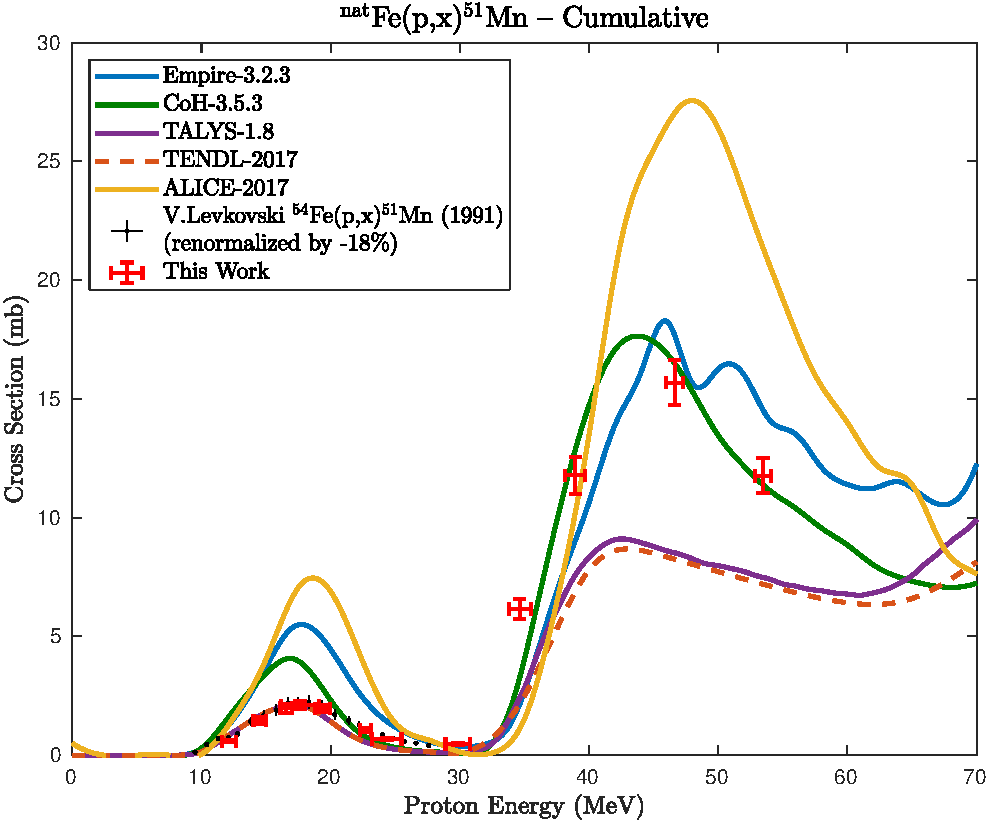
\includegraphics[width=0.5\textwidth]{./figures/51Mn.pdf}
 % Nb_ptallies.pdf: 380x298 pixel, 72dpi, 13.41x10.51 cm, bb=0 0 380 298
 \caption{Measured \ce{^{nat}Fe}(p,x)\ce{^{51}Mn} cross section, with the \ce{^{54}Fe}(p,$\alpha$)\ce{^{51}Mn} reaction channel visibly peaking at approximately \mbox{15 MeV}.}
 \label{fig:51Mn}
\end{figure}





\begin{figure}[h]
 \centering
 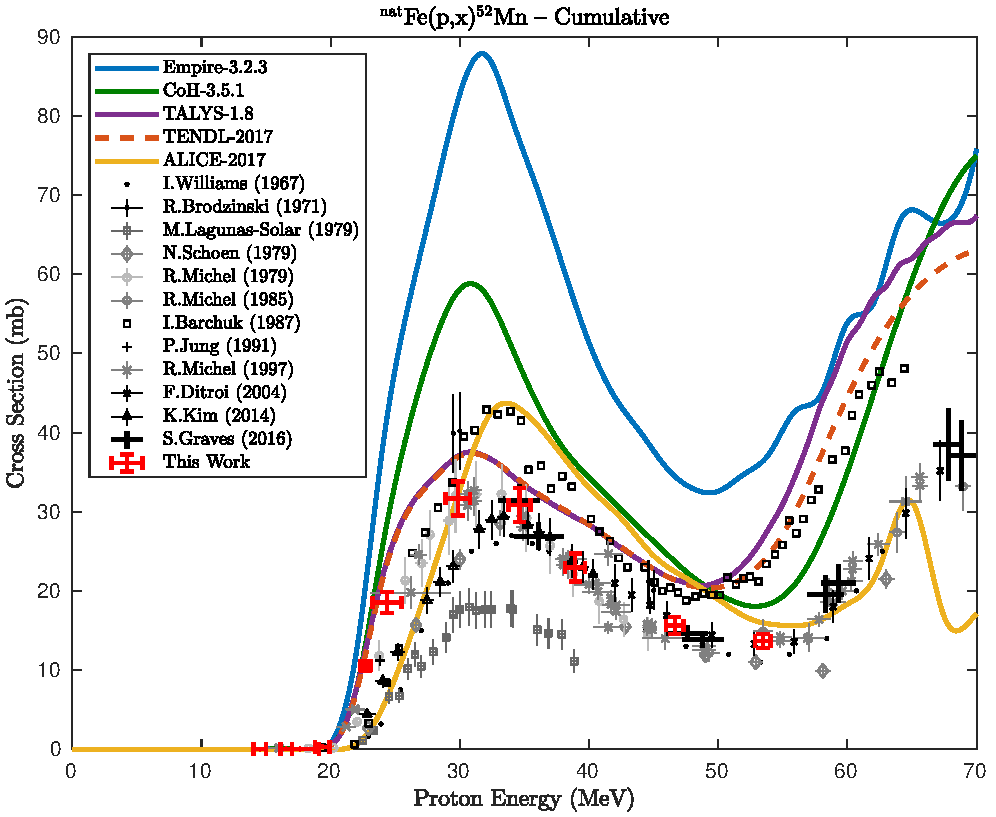
\includegraphics[width=0.5\textwidth]{./figures/52Mn.pdf}
 % Nb_ptallies.pdf: 380x298 pixel, 72dpi, 13.41x10.51 cm, bb=0 0 380 298
 \caption{Measured \ce{^{nat}Fe}(p,x)\ce{^{52}Mn} cross section, with \ce{^{56}Fe}(p,$\alpha$n)\ce{^{52}Mn}/\ce{^{54}Fe}(p,2pn)\ce{^{52}Mn} reaction channels visibly peaking at approximately \mbox{30 MeV}.}
 \label{fig:temp_52Mn}
\end{figure}


For this analysis, the focus will be on the three largest channels  measured -- \ce{^{nat}Fe}(p,x)\ce{^{51}Mn}, \ce{^{nat}Fe}(p,x)\ce{^{52m}Mn}, and \ce{^{nat}Fe}(p,x)\ce{^{52}Mn}.
The use of natural abundance targets in these measurements exacerbates the modeling  challenges seen in our previous work using monoisotopic targets\,\cite{Voyles2018a}, by propagating the difficulties inherent to modeling a wide number of reaction channels, to multiple target isotopes.
As a result, this analysis is useful for a qualitative comparison of predictive capabilities, but no firm conclusions can be drawn about the direct causes of any inaccuracies, as there are many \enquote{moving parts} in these calculations.
% However, no firm conclusions can be drawn about the direct causes of the inaccuracies, as there are many \enquote{moving parts} in these calculations, with measurements performed using natural abundance targets.
For the \ce{^{nat}Fe}(p,x)\ce{^{51}Mn} reactions, seen in \autoref{fig:51Mn}, the lower-energy  \ce{^{54}Fe}(p,$\alpha$)\ce{^{51}Mn} reaction, which peaks around 15\,MeV, is  well-modeled by TALYS and TENDL, and over-predicted by EMPIRE, CoH and ALICE.
The higher-energy reactions on the higher mass Fe isotopes, however, are better matched by  EMPIRE and CoH.
ALICE overpredicts the production of \ce{^{51}Mn} in both peaks, and appears to peak at too high an energy.
As was seen in the modeling of high-energy proton-induced niobium reactions\,\cite{Voyles2018a}, TALYS and TENDL do well with the lower-energy \enquote{compound} reactions but do not accurately predict the higher-energy reactions that have a significant pre-equilibrium component.
EMPIRE and CoH seem to accurately predict the locations of the peaks, but often fail to reliably estimate the magnitude of the cross section.
This is seen again in the  \ce{^{nat}Fe}(p,x)\ce{^{52}Mn} cross section, where the first peak is well-modeled by TALYS and TENDL, but  rises much more rapidly than the data would support above 50\,MeV.
CoH and EMPIRE, again, overpredict the cross sections at all energies, but seem to have the correct shape.
Through measurement of the  \ce{^{nat}Fe}(p,x)\ce{^{52m}Mn} independent cross section, the effect of spin distributions in highly-excited nuclear states can be studied.
The measured data suggest that the independent cross section to the $2^+$ isomer should be a large fraction of the cumulative cross section to \ce{^{52}Mn} (which has a $6^+$ ground state), over 80\% at the peak energy.
All three codes predict about 50\%, which indicates that the isomer feeding is not well-modeled.
It is possible that this is caused by residual nucleus population and/or level density models that are skewed too heavily towards high spin.
In the other isomer-to-ground state ratio measured for Fe,  \ce{^{nat}Fe}(p,x)\ce{^{58}Co}, the opposite is seen -- the codes underpredict the ratio of the isomer-to-ground state, but in this case the isomer is the higher spin state ($5^+$, compared with a  $2^+$ ground state).
Given that the level density model was the same for all of the product nuclei, it points to the spin distribution of the initial population of the residual nucleus as the main problem with modeling.
% However, no firm conclusions can be drawn about the direct causes of the inaccuracies, as there are many \enquote{moving parts} in these calculations, with measurements performed using natural abundance targets.


% 
% 
% 
% % In this work
% Cumulative cross sections are reported here for the first observable product nuclei in a mass chain, or whenever it is impossible to use decay spectrometry to distinguish direct production of a nucleus from decay feeding.
% For all remaining observed reaction products in the mass chain, and cases where no decay precursors exist, independent cross sections are reported, allowing for determination of the direct production via subtraction.  
% This, in turn, offers the opportunity to 
% % use these data to gain insight into 
% gauge the predictive capabilities of modern nuclear models used in the reaction evaluation process.  
% The reaction channels with independent cross sections were compared to calculations with the reaction modeling codes EMPIRE, TALYS, and CoH, run with the default settings. 
% The default optical models and E1 gamma strength function models for each code are presented in Table \ref{tab:fe_defaults}. 
% The large energy range covered by many of the exit channels, which extends significantly beyond the range of pure compound nuclear/evaporation, allows the data to be used to study the differences between these modeling codes in the  pre-equilibrium regime.
% % All three codes use a two-exciton phenomenological model to calculate the pre-equilibrium cross section, but the specific implementation differs between the codes. 
% 
% 
% The default level density in both CoH and TALYS is the Gilbert-Cameron model, which uses a Constant Temperature model below a critical energy and Fermi Gas model above it.
% %\,\cite{add_level_density_models_here}. 
% The default level density in EMPIRE is the Enhanced Generalized Superfluid Model (EGSM) which uses the Generalized Superfluid model below a critical energy, and Fermi Gas model above it\,\cite{Capote2009}.
% %\,\cite{add_level_density_models_here}.
% The EGSM densities are normalized to $D_0$ and the discrete levels, but in such a way that only the level density below the neutron separation energy is  effected by the discrete levels chosen for the normalization.  
% All three codes use a two-exciton phenomenological model to calculate the pre-equilibrium cross section, but the specific implementation differs between the codes. 


% % The modeling of several of the \ce{^{93}Nb} residual production cross sections are studied in detail here. 
% % Only total channel residual 
% Given the large number of exit channels in this data set, we will limit our discussion to  cross sections for the production of a specific residual nucleus with experimental data through the full rise and fall of the peak, 
% % that have only one reaction channel, and that are 
% and at least 1\% of the total reaction cross section.
% % are discussed in detail. 
% % Residual production
% Exit channel cross sections that do not exhibit the full rise and fall of the peak, which is identified as 
% % the compound portion of the cross section
% being dominated by the formation of a compound nucleus, do not provide enough information to analyze the calculations.
% % Some residuals, such as 
% Residual nuclei like \ce{^{88}Zr} that can be produced by multiple reaction channels, such as (p,$\alpha$2n) and by (p,2p4n)  are also not discussed in depth. 
% % Both compound peaks are seen in the data and cannot be separated, so such residuals are not included in the detailed analysis.
% % Very small channels, 
% We exclude reactions with cross sections with peak values less than 1\% of the total reaction cross section 
% % are excluded because the modeling of their cross sections is 
% because their behavior is extremely sensitive  to  more dominant  channels.
% The three residual nuclei that meet all of the above criteria for which there is an independent measurement of the residual production cross section are \ce{^{86}Y}, \ce{^{90}Mo}, and \ce{^{90}Nb}.
% 
% 
% The \ce{^{93}Nb}(p,$\alpha$p3n)\ce{^{86}Y} reaction channel, which peaks at approximately \mbox{70\,MeV}, is well within the compound regime for the entire energy region of this experiment (\autoref{fig:86Y}).
% The data collected on this residual is consistent with the one other data set available, taken in 1997 by Michel \emph{et al.}\,\cite{MICHEL1997153}. 
% The \ce{^{93}Nb}(p,4n)\ce{^{90}Mo} and \ce{^{93}Nb}(p,p3n)\ce{^{90}Nb} channels both peak early in the energy region, around 50\,MeV, and the data clearly show the full rise, peak, and fall of the compound cross section (\autoref{fig:90Mo} \& \ref{fig:90Nb}). 
% In both of these channels, this data  is consistent with the data by Titarenko \emph{et al.} in 2011\,\cite{Titarenko2011}.
% 
% The \ce{^{90}Nb} production cross section exhibits a persistent pre-equilibrium \enquote{tail} that keeps the channel open  well after the compound cross section has fallen away. 
% TALYS, TENDL, and CoH seem to have the correct shape for this pre-equilibrium cross section, with magnitudes that are just slightly too low.
% EMPIRE, however, does not level off  as much as the data and the other codes are seen to, and misses the high-energy data points.




\begin{figure}[h]
 \centering
 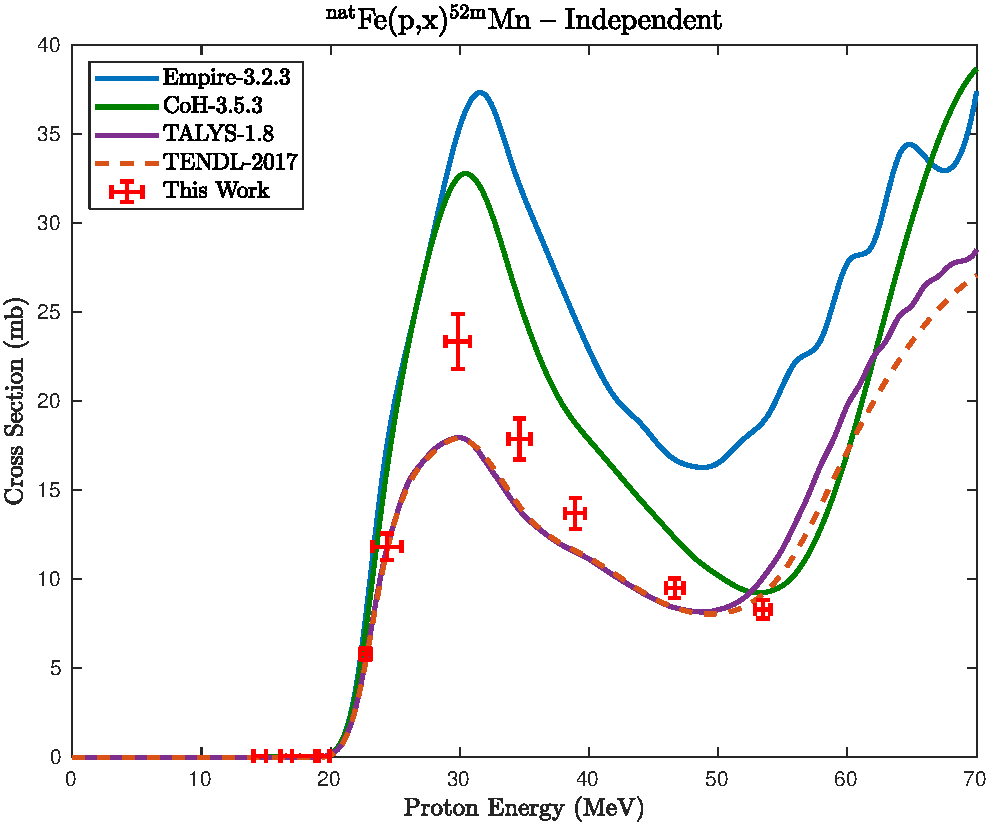
\includegraphics[width=0.5\textwidth]{./figures/52mMn.pdf}
 % Nb_ptallies.pdf: 380x298 pixel, 72dpi, 13.41x10.51 cm, bb=0 0 380 298
 \caption{Measured \ce{^{nat}Fe}(p,x)\ce{^{52m}Mn} cross section, with the \ce{^{56}Fe}(p,$\alpha$n)\ce{^{52m}Mn}/\ce{^{54}Fe}(p,2pn)\ce{^{52m}Mn} reaction channels visibly peaking at approximately \mbox{30 MeV}.}
 \label{fig:temp_52mMn}
\end{figure}



% 
% In all three channels, the TALYS, TENDL, and CoH calculations rise, peak, and fall at lower energies than the data, while EMPIRE calculates the peak to occur at higher energies.
% For \ce{^{90}Mo}, the EMPIRE peak is representative of the data.
% For \ce{^{86}Y} and \ce{^{90}Nb}, the peak is missed by all three  of the codes.
% 
% 
% The magnitudes of the TALYS and TENDL calculations are consistently too low in the three channels studied here. 
% For \ce{^{86}Y}, CoH and EMPIRE also predict smaller cross sections than the data would suggest, which may be influenced by incorrect modeling of other, stronger, channels.
% The magnitude of the peak in the CoH calculation for \ce{^{90}Mo}  is consistent  with the data, while EMPIRE predicts a cross section that is approximately the same magnitude as that of TALYS.
% \ce{^{90}Nb} is one of the strongest measured channels, approximately 10\% of the total reaction cross section, and the values from the three codes are all consistent, but  too small, in magnitude.





 
 \section{\label{sec:conclusions_fe}Conclusions}
 

We present here a set of measurements of 34 cross sections for the \ce{^{nat}Fe}(p,x), \ce{^{nat}Cu}(p,x), and  \ce{^{nat}Ti}(p,x) reactions up to 55\,MeV, as well as  independent measurements of three isomer branching ratios.
Nearly all cross sections have been reported with higher precision than previous measurements.
We report the first measurements  for $\leq$70\,MeV protons  of the  \ce{^{nat}Fe}(p,x)\ce{^{49}Cr}, \ce{^{nat}Fe}(p,x)\ce{^{51}Mn}, \ce{^{nat}Fe}(p,x)\ce{^{52m}Mn},  \ce{^{nat}Fe}(p,x)\ce{^{56}Mn}, and \ce{^{nat}Fe}(p,x)\ce{^{58m}Co} reactions, as well as the first measurement of the independent cross sections for    \ce{^{nat}Fe}(p,x)\ce{^{51}Cr}, \ce{^{nat}Fe}(p,x)\ce{^{52g}Mn}, \ce{^{nat}Fe}(p,x)\ce{^{58g}Co}, and the \ce{^{52\text{m}}Mn} ($2^+$) / \ce{^{52\text{g}}Mn}  ($6^+$) and \ce{^{58\text{m}}Co} ($5^+$) / \ce{^{58\text{g}}Co}  ($2^+$)  isomer branching ratios via \ce{^{nat}Fe}(p,x).
% We advise that future activation experiments avoid the use of silicone-based adhesives, particularly in conjunction with aluminum monitor foils, to avoid reporting an enhanced fluence due to \ce{^{22,24}Na} contamination.
We also use these measurements to illustrate the deficiencies in the current state of  reaction modeling up to 55\,MeV for  \ce{^{nat}Fe}(p,x), \ce{^{nat}Cu}(p,x), and  \ce{^{nat}Ti}(p,x) reactions.
Finally, this work provides another example of the current issues with modeling of  stopping power in stacked target charged particle irradiation experiments, corrected using variance minimization techniques.  
% usefulness of the recently-described variance minimization techniques for reducing energy uncertainties in stacked target charged particle irradiation experiments.



% 
% \paragraph{Syntax}
% The argument of \verb+\cite+ may be a single \emph{key}, 
% or may consist of a comma-separated list of keys.
% The citation \emph{key} may contain 
% letters, numbers, the dash (-) character, or the period (.) character. 
% New with natbib 8.3 is an extension to the syntax that allows for 
% a star (*) form and two optional arguments on the citation key itself.
% The syntax of the \verb+\cite+ command is thus (informally stated)
% \begin{quotation}\flushleft\leftskip1em
% \verb+\cite+ \verb+{+ \emph{key} \verb+}+, or\\
% \verb+\cite+ \verb+{+ \emph{optarg+key} \verb+}+, or\\
% \verb+\cite+ \verb+{+ \emph{optarg+key} \verb+,+ \emph{optarg+key}\ldots \verb+}+,
% \end{quotation}\noindent
% where \emph{optarg+key} signifies 
% \begin{quotation}\flushleft\leftskip1em
% \emph{key}, or\\
% \texttt{*}\emph{key}, or\\
% \texttt{[}\emph{pre}\texttt{]}\emph{key}, or\\
% \texttt{[}\emph{pre}\texttt{]}\texttt{[}\emph{post}\texttt{]}\emph{key}, or even\\
% \texttt{*}\texttt{[}\emph{pre}\texttt{]}\texttt{[}\emph{post}\texttt{]}\emph{key}.
% \end{quotation}\noindent
% where \emph{pre} and \emph{post} is whatever text you wish to place 
% at the beginning and end, respectively, of the bibliographic reference
% % (see Ref.~[\onlinecite{witten2001}] and the two under Ref.~[\onlinecite{feyn54}]).
% (Keep in mind that no automatic space or punctuation is applied.)
% It is highly recommended that you put the entire \emph{pre} or \emph{post} portion 
% within its own set of braces, for example: 
% \verb+\cite+ \verb+{+ \texttt{[} \verb+{+\emph{text}\verb+}+\texttt{]}\emph{key}\verb+}+.
% The extra set of braces will keep \LaTeX\ out of trouble if your \emph{text} contains the comma (,) character.
% 
% The star (*) modifier to the \emph{key} signifies that the reference is to be 
% merged with the previous reference into a single bibliographic entry, 
% % a common idiom in APS and AIP articles (see below, Ref.~[\onlinecite{epr}]). 
% When references are merged in this way, they are separated by a semicolon instead of 
% the period (full stop) that would otherwise appear.
% 
% \paragraph{Eliding repeated information}
% When a reference is merged, some of its fields may be elided: for example, 
% when the author matches that of the previous reference, it is omitted. 
% If both author and journal match, both are omitted.
% If the journal matches, but the author does not, the journal is replaced by \emph{ibid.},
% % as exemplified by Ref.~[\onlinecite{epr}]. 
% These rules embody common editorial practice in APS and AIP journals and will only
% be in effect if the markup features of the APS and AIP Bib\TeX\ styles is employed.
% 
% \paragraph{The options of the cite command itself}
% Please note that optional arguments to the \emph{key} change the reference in the bibliography, 
% not the citation in the body of the document. 
% For the latter, use the optional arguments of the \verb+\cite+ command itself:
% \verb+\cite+ \texttt{*}\allowbreak
% \texttt{[}\emph{pre-cite}\texttt{]}\allowbreak
% \texttt{[}\emph{post-cite}\texttt{]}\allowbreak
% \verb+{+\emph{key-list}\verb+}+.



 \section{Acknowledgements}
 
%  Stephen Graves - consulting for methodology, guidance.
 
 The authors would like to particularly acknowledge the assistance and support of  
%  Michael Gallegos and Don Dry in the LANL C-NR Countroom, David Reass and Mike Connors at LANSCE-IPF, and the LANSCE Accelerator Operations staff. 
(mention staff of the 88 )
 
% We gratefully acknowledge support for this work from the United States Department of Energy, Office of Science via the Isotope Development and Production for Research and Applications subprogram in the Office of Nuclear Physics. 
This work has been carried out  under the auspices of the U.S. Department of Energy by  Lawrence Berkeley National Laboratory and the U.S. Nuclear Data Program under contract \# DE-AC02-05CH11231.
This research was performed under appointment to the Rickover Fellowship Program in Nuclear Engineering, sponsored by the Naval Reactors Division of the U.S. Department of Energy
Additional support has been provided by the U.S. Nuclear Regulatory Commission.



 
This research used the Savio computational cluster resource provided by the Berkeley Research Computing program at the University of California, Berkeley (supported by the UC Berkeley Chancellor, Vice Chancellor for Research, and Chief Information Officer).



% % \pagebreak
% % 
% % \onecolumn
% % 
\appendix



% \section{Decay data} \label{sec:fe_data}
% % 
% % % \begin{longtable}{|c|c|c|c|c|} 
% % % \caption{My caption}
% % % \label{tab:dummy}
% % % % \begin{tabular}{|c|c|c|c|c|}
% % %    \hline
% % %  
% % % \end{longtable}
% % Table of decay data  for observed gamma-rays. 
% The   lifetimes and gamma-ray branching ratios  listed in these tables were used for all calculations of measured cross sections reported in this work, and have been taken from the most recent edition of  Nuclear Data Sheets for each  mass chain 
% % \cite{Basunia2015,Firestone2007,Wang2017,Dong2015,Dong2014,JUNDE2008787,Junde2011,Bhat1998,Nesaraja2010,BAGLIN2002,Browne2013,Zuber20151,NICHOLS2012973,Singh2007,Browne2010,Tuli2003,McCutchan2015,Singh2014,NEGRET20151,Johnson2015,McCutchan2014,Singh2013,Browne1997,Baglin2013,Baglin2012,Baglin2011}. 
% 
% 
% 
% % Preview source code for paragraph 0
% 
% \begin{table}[ht]
% \centering
% \caption{Decay data for gamma-rays observed in \ce{^{nat}Ti}(p,x) and \ce{^{nat}Cu}(p,x).}
% \label{tab:fe_nudat_table_monitors}
% \small
% % \resizebox{\textheight}{!}{%
% % Disable adjustbox for journal submission
% % \begin{adjustbox}{totalheight=\textheight-2\baselineskip}
% \begin{tabular}{@{}llll@{}}
% \toprule
% % \begin{tabular}{|c|c|c|c|}
% % \hline 
% Nuclide & Half-life & E$_\gamma$ (keV) & I$_\gamma$ (\%)\\
% \midrule
% \ce{^{22}Na} & 2.6018(22) y & 1274.537 & 99.940(14)\\
%  
% % \ce{^{24}Na} & 14.997(12) h & 1368.626 & 99.9936(15)\\
% %  
% % \ce{^{51}Cr} & 27.704(3) d & 320.0824 & 9.910(10)\\
% %  
% % \ce{^{52m}Mn} & 21.1(2) m & 1434.0600 & 98.2(5)\\
% %  
% % \ce{^{52}Mn} & 5.591(3) d & 744.233 & 90.0(12)\\
% %  
% %  & 5.591(3) d & 935.544 & 94.5(13)\\
% %  
% %  & 5.591(3) d & 1246.278 & 4.21(7)\\
% %  
% %  & 5.591(3) d & 1434.092 & 100.0(14)\\
% %  
% % \ce{^{54}Mn} & 312.20(20) & 834.848 & 99.9760(10)\\
% %  
% % \ce{^{55}Co} & 17.53(3) h & 477.2 & 20.2(17)\\
% %  
% %  & 17.53(3) h & 931.1 & 75.0(35)\\
% %  
% %  & 17.53(3) h & 1316.6 & 7.1(3)\\
% %  
% %  & 17.53(3) h & 1408.5 & 16.9(8)\\
% %  
% % \ce{^{56}Ni} & 6.075(10) d & 158.38 & 98.8(10)\\
% %  
% %  & 6.075(10) d & 269.50 & 36.5(8)\\
% %  
% %  & 6.075(10) d & 480.44 & 36.5(8)\\
% %  
% %  & 6.075(10) d & 749.95 & 49.5(12)\\
% %  
% %  & 6.075(10) d & 811.85 & 86.0(9)\\
% %  
% %  & 6.075(10) d & 1561.80 & 14.0(6)\\
% %  
% % \ce{^{56}Co} & 77.236(26) d & 846.770 & 99.9399(2)\\
% %  
% % %  & 77.236(26) d & 977.372 & 1.421(6)\\
% %  
% %  & 77.236(26) d & 1037.843 & 14.05(4)\\
% %  
% %  & 77.236(26) d & 1238.288 & 66.46(12)\\
% %  
% %  & 77.236(26) d & 1360.212 & 4.283(12)\\
% %  
% %  & 77.236(26) d & 1771.357 & 15.41(6)\\
% %  
% % \ce{^{57}Ni} & 35.60(6) h & 127.164 & 16.7(5)\\
% %  
% %  & 35.60(6) h & 1377.63 & 81.7(24)\\
% %  
% %  & 35.60(6) h & 1757.55 & 5.75(20)\\
% %  
% %  & 35.60(6) h & 1919.52 & 12.3(4)\\
% %  
% % \ce{^{57}Co} & 271.74(6) d & 122.06065 & 85.60(17)\\
% %  
% %  & 271.74(6) d & 136.47356 & 10.68(8)\\
% %  
% % \ce{^{58}Co} & 70.86(6) d & 810.7593 & 99.450(10)\\
% %  
% %  & 70.86(6) d & 863.951 & 0.686(10)\\
% %  
% % %  & 70.86(6) d & 1674.725 & 0.517(10)\\
% %  
% % \ce{^{59}Fe} & 44.495(9) d & 1099.245 & 56.5(18)\\
% %  
% %  & 44.495(9) d & 1291.590 & 43.2(14)\\
% %  
% % \ce{^{60}Co} & 5.2714(5) y & 1173.228 & 99.85(3)\\
% %  
% %  & 5.2714(5) y & 1332.492 & 99.9826(6)\\
% %  
% % \ce{^{61}Cu} & 3.339(8) h & 282.956 & 12.2(2.2)\\
% %  
% %  & 3.339(8) h & 373.050 & 2.1(4)\\
% %  
% % %  & 3.339(8) h & 588.605 & 1.17(21)\\
% %  
% %  & 3.339(8) h & 656.008 & 10.8(20)\\
% %  
% %  & 3.339(8) h & 1185.234 & 3.7(7)\\
% %  
% % \ce{^{62}Zn} & 9.193(15) h & 243.36 & 2.52(23)\\
% %  
% %  & 9.193(15) h & 246.95 & 1.90(18)\\
% %  
% %  & 9.193(15) h & 260.43 & 1.35(13)\\
% %  
% % %  & 9.193(15) h & 304.88 & 0.29(3)\\
% %  
% % %  & 9.193(15) h & 349.60 & 0.45(4)\\
% %  
% %  & 9.193(15) h & 394.03 & 2.24(17)\\
% %  
% %  & 9.193(15) h & 548.35 & 15.3(14)\\
% %  
% %  & 9.193(15) h & 596.56 & 26.0(20)\\
% %  
% % %  & 9.193(15) h & 637.41 & 0.25(3)\\
% %  
% % \ce{^{64}Cu} & 12.701(2) h & 1345.77 & 0.475(11)\\
% %  
% % \ce{^{65}Zn} & 243.93(9) d & 1115.539 & 50.04(10)\\
% \bottomrule
% \end{tabular}
% % }
% % \end{adjustbox}
% \end{table}
% 
% 
% 
% \begin{table}[ht]
% \centering
% \caption{Decay data for gamma-rays observed in \ce{^{nat}Fe}(p,x).}
% \label{tab:fe_nudat_table_nb}
% \small
% % \resizebox{\textheight}{!}{%
% % Disable adjustbox for journal submission
% % \begin{adjustbox}{totalheight=\textheight-2\baselineskip}
% \begin{tabular}{@{}llll@{}}
% \toprule
% % \begin{tabular}{|c|c|c|c|}
% % \hline 
% Nuclide & Half-life & E$_\gamma$ (keV) & I$_\gamma$ (\%)\\
% \midrule
% \ce{^{82m}Rb} & 6.472(6) h & 554.35 & 62.4(9)\\
%  
%  & 6.472(6) h & 619.11 & 37.98(9)\\
%  
% %  & 6.472(6) h & 698.37 & 26.3(7)\\
%  
% %  & 6.472(6) h & 776.52 & 84.39(21)\\
% %  
% %  & 6.472(6) h & 1044.08 & 32.07(8)\\
% %  
% % %  & 6.472(6) h & 1317.43 & 23.7(6)\\
% %  
% % \ce{^{83}Sr} & 32.41(3) h & 418.37 & 4.2(3)\\
% %  
% %  & 32.41(3) h & 762.65 & 26.7(22)\\
% %  
% % \ce{^{85m}Y} & 4.86(13) h & 231.7 & 22.8(22)\\
% %  
% % \ce{^{85}Y} & 2.68(5) h & 231.65 & 84(9)\\
% %  
% %  & 2.68(5) h & 913.89 & 9.0(9)\\
% %  
% % \ce{^{86}Zr} & 16.5(1) h & 242.8 & 95.84(2)\\
% %  
% %  & 16.5(1) h & 612.0 & 5.8(3)\\
% %  
% % % \ce{^{86}Y} & 14.74(2) h & 187.87 & 1.26(4)\\
% % \ce{^{86}Y}  & 14.74(2) h & 443.13 & 16.9(5)\\
% % 
% %  
% % %  & 14.74(2) h & 190.80 & 1.01(3)\\
% %  
% % %  & 14.74(2) h & 307.00 & 3.47(8)\\
% %  
% % %  & 14.74(2) h & 443.13 & 16.9(5)\\
% %  
% % %  & 14.74(2) h & 580.57 & 4.78(14)\\
% %  
% % %  & 14.74(2) h & 608.29 & 2.01(15)\\
% %  
% %  & 14.74(2) h & 627.72 & 32.6(1)\\
% %  
% % %  & 14.74(2) h & 703.33 & 15.4(4)\\
% %  
% % %  & 14.74(2) h & 709.90 & 2.62(8)\\
% %  
% % %  & 14.74(2) h & 767.63 & 2.4(3)\\
% %  
% % %  & 14.74(2) h & 835.67 & 4.4(6)\\
% %  
% % %  & 14.74(2) h & 1024.04 & 3.79(17)\\
% %  
% %  & 14.74(2) h & 1076.63 & 82.5(4)\\
% %  
% %  & 14.74(2) h & 1153.05 & 30.5(9)\\
% %  
% % %  & 14.74(2) h & 1163.03 & 1.18(4)\\
% % %  
% % %  & 14.74(2) h & 1253.11 & 1.53(5)\\
% %  
% % %  & 14.74(2) h & 1349.15 & 2.95(9)\\
% %  
% %  & 14.74(2) h & 1854.38 & 17.2(5)\\
% %  
% %  & 14.74(2) h & 1920.72 & 20.8(7)\\
% %  
% % \ce{^{87}Zr} & 1.68(1) h & 380.79 & 62.79(10)\\
% %  
% %  & 1.68(1) h & 1227.0 & 2.80(4)\\
% %  
% % \ce{^{87m}Y} & 13.37(1) h & 380.79 & 78.05(8)\\
% %  
% % \ce{^{87}Y} & 79.8(3) h & 388.5276 & 82.2(7)\\
% %  
% %  & 79.8(3) h & 484.805 & 89.8(9)\\
% %  
% % \ce{^{88}Zr} & 83.4(3) d & 392.87 & 97.29(14)\\
% %  
% % \ce{^{88}Y} & 106.627(21) d & 898.042 & 93.7(3)\\
% %  
% %  & 106.627(21) d & 1836.063 & 99.2(3)\\
% %  
% % \ce{^{89m}Nb} & 66(2) m & 588.0 & 95.57(13)\\
% %  
% % \ce{^{89}Nb} & 2.03(7) h & 1511.4 & 1.9(4)\\
% %  
% %  & 2.03(7) h & 1627.2 & 3.5(7)\\
% %  
% %  & 2.03(7) h & 1833.4 & 3.3(7)\\
% %  
% % \ce{^{89}Zr} & 78.41(12) h & 909.15 & 99.04(3)\\
% %  
% %  & 78.41(12) h & 1713.0 & 0.745(13)\\
% %  
% % %  & 78.41(12) h & 1744.5 & 0.123(4)\\
% %  
% % \ce{^{90}Mo} & 5.56(9) h & 122.370 & 64(3)\\
% %  
% %  & 5.56(9) h & 162.93 & 6.0(6)\\
% %  
% %  & 5.56(9) h & 203.13 & 6.4(6)\\
% %  
% %  & 5.56(9) h & 257.34 & 78(4)\\
% %  
% %  & 5.56(9) h & 323.20 & 6.3(6)\\
% %  
% %  & 5.56(9) h & 472.2 & 1.42(16)\\
% %  
% %  & 5.56(9) h & 941.5 & 5.5(7)\\
% %  
% % \ce{^{90}Nb} & 14.6(5) h & 132.716 & 4.13(4)\\
% %  
% %  & 14.6(5) h & 141.178 & 66.8(7)\\
% %  
% % %  & 14.6(5) h & 890.64 & 1.80(4)\\
% %  
% %  & 14.6(5) h & 1611.76 & 2.38(7)\\
% %  
% % %  & 14.6(5) h & 1913.194 & 1.280(17)\\
% %  
% % \ce{^{91m}Nb} & 60.86(22) d & 104.62 & 0.574(1)\\
% %  
% %  & 60.86(22) d & 1204.67 & 2.0(3)\\
% %  
% % \ce{^{92m}Nb} & 10.15(2) d & 912.6 & 1.78(10)\\
% %  
% %  & 10.15(2) d & 934.44 & 99.15(4)\\
% %  
% % \ce{^{93m}Mo} & 6.85(7) d & 263.049 & 57.4(11)\\
% %  
% %  & 6.85(7) d & 684.693 & 99.9(8)\\
% %  
% %  & 6.85(7) d & 1477.138 & 99.1(11)\\
% \bottomrule
% \end{tabular}
% % }
% % \end{adjustbox}
% \end{table}
% 

\pagebreak



% 
% 
\section{Stack design } \label{sec:fe_stack_design}

% Plots of the isomer-to-ground state ratios measured in this work are presented here, in comparison with literature data and reaction modeling codes 
% \cite{Michel1978,Kopecky1993,Zarie2006a,Khandaker2009}.





% Combined table
% Please add the following required packages to your document preamble:
% \usepackage{booktabs}
\begin{table*}[h!]
\centering
\caption{Specifications of the 25\,MeV and 55\,MeV target stack designs in the present work. The proton beam enters the stack upstream of the SS-5 and SS-3 profile monitors, respectively, and travels through the stack in the order presented here. The 6061 aluminum degraders have a measured density of approximately 2.68 $\pm$ 0.03 g/cm$^3$. Their areal densities were determined using the variance minimization techniques described  in this work  and an earlier paper\,\cite{Voyles2018a}. 
% the earlier paper by Graves \etal\\,\cite{Graves2016}.
A 316 stainless steel foil is inserted at both the front and rear of each target stack as a monitor of the beam's spatial profile, by developing radiochromic film (Gafchromic EBT3) after end-of-bombardment.
% (EOB).
All Fe/Ti/Cu activation foils were each covered on both sides by 3M 5413-Series Kapton polyimide film tape,  
each piece of tape 
consisting of 43.2 \mmicro m of a silicone adhesive (nominal 4.79\,mg/cm$^2$) on 25.4 \mmicro m of a polyimide backing (nominal 3.61\,mg/cm$^2$).
Similarly to the aluminum degraders, the effective areal density of the Kapton tape was determined through variance minimization, suggesting an effective 5.69\% enhancement of the nominal values.}
\label{tab:fe_stack_table}
\small
\resizebox{\textwidth}{!}{%
\begin{tabular}{@{}lll|lll@{}}
\toprule\toprule
% Target Layer       & Nominal Thickness & Measured thickness (mg/cm\textasciicircum 2) & Thickness Uncertainty (\%) \\ \midrule
25\,MeV Target layer            & \begin{tabular}[c]{@{}l@{}}Measured \\ thickness\end{tabular} & \begin{tabular}[c]{@{}l@{}}Measured\\areal density\\(mg/cm$^2$)\end{tabular} & 
% \begin{tabular}[c]{@{}l@{}}Uncertainty \\ in areal\\ density  (\%)\end{tabular} 
55\,MeV Target layer            & \begin{tabular}[c]{@{}l@{}}Measured \\ thickness\end{tabular} & \begin{tabular}[c]{@{}l@{}}Measured\\areal density\\(mg/cm$^2$)\end{tabular} 
% & \begin{tabular}[c]{@{}l@{}}Uncertainty \\ in areal\\ density  (\%)\end{tabular} 
\\
\midrule
SS profile monitor SS-5 & 130.94 \mmicro m                                              & 100.57                                                                      $\pm$ 0.17\%                                                                      & SS profile monitor SS-3 & 130.9 \mmicro m                                               & 100.48                                                                      $\pm$ 0.17\%                                                                      \\
Fe-08                   & 26.25 \mmicro m                                               & 19.69                                                                       $\pm$ 0.17\%                                                                      & Fe-01                   & 25.75 \mmicro m                                               & 20.22                                                                       $\pm$ 0.21\%                                                                      \\
Ti-14                   & 25.01 \mmicro m                                               & 10.87                                                                       $\pm$ 0.36\%                                                                      & Ti-01                   & 25.88 \mmicro m                                               & 11.09                                                                       $\pm$ 0.16\%                                                                      \\
Cu-14                   & 24.01 \mmicro m                                               & 17.49                                                                       $\pm$ 0.40\%                                                                      & Cu-01                   & 28.81 \mmicro m                                               & 22.40                                                                       $\pm$ 0.11\%                                                                      \\
Al Degrader E-09        & 256.5 \mmicro m                                               & --                                                                                                                                                  & Al Degrader A-1         & 2.24 mm                                                       & --                                                                                                                                                  \\
Fe-09                   & 26.5 \mmicro m                                                & 19.90                                                                       $\pm$ 0.09\%                                                                      & Fe-02                   & 25.5 \mmicro m                                                & 19.91                                                                       $\pm$ 0.13\%                                                                      \\
Ti-15                   & 23.81 \mmicro m                                               & 10.97                                                                       $\pm$ 0.11\%                                                                      & Ti-02                   & 25.74 \mmicro m                                               & 10.94                                                                       $\pm$ 0.24\%                                                                      \\
Cu-15                   & 21.81 \mmicro m                                               & 17.63                                                                       $\pm$ 0.46\%                                                                      & Cu-02                   & 28.75 \mmicro m                                               & 22.32                                                                       $\pm$ 0.40\%                                                                      \\
Al Degrader H-01        & 127.09 \mmicro m                                              & --                                                                                                                                                  & Al Degrader A-2         & 2.24 mm                                                       & --                                                                                                                                                  \\
Fe-10                   & 26.5 \mmicro m                                                & 19.84                                                                       $\pm$ 0.11\%                                                                      & Fe-03                   & 25.25 \mmicro m                                               & 20.00                                                                       $\pm$ 0.27\%                                                                      \\
Ti-16                   & 24.6 \mmicro m                                                & 10.96                                                                       $\pm$ 0.32\%                                                                      & Ti-03                   & 25.91 \mmicro m                                               & 11.25                                                                       $\pm$ 0.15\%                                                                      \\
Cu-16                   & 22.01 \mmicro m                                               & 17.22                                                                       $\pm$ 0.25\%                                                                      & Cu-03                   & 28.86 \mmicro m                                               & 22.49                                                                       $\pm$ 0.20\%                                                                      \\
Fe-11                   & 27.26 \mmicro m                                               & 19.96                                                                       $\pm$ 0.17\%                                                                      & Al Degrader C-1         & 0.97 mm                                                       & --                                                                                                                                                  \\
Ti-17                   & 25.01 \mmicro m                                               & 10.88                                                                       $\pm$ 0.25\%                                                                      & Fe-04                   & 25.25 \mmicro m                                               & 19.93                                                                       $\pm$ 0.33\%                                                                      \\
Cu-17                   & 28.82 \mmicro m                                                  & 21.91                                                                       $\pm$ 0.33\%                                                                      & Ti-04                   & 25.84 \mmicro m                                               & 10.91                                                                       $\pm$ 0.18\%                                                                      \\
Fe-12                   & 27.01 \mmicro m                                               & 20.03                                                                       $\pm$ 0.12\%                                                                      & Cu-04                   & 28.78 \mmicro m                                               & 22.38                                                                       $\pm$ 0.29\%                                                                      \\
Ti-18                   & 25.01 \mmicro m                                               & 11.00                                                                       $\pm$ 0.87\%                                                                      & Al Degrader C-2         & 0.97 mm                                                       & --                                                                                                                                                  \\
Cu-18                   & 28.75 \mmicro m                                               & 22.33                                                                       $\pm$ 0.14\%                                                                      & Fe-05                   & 25.64 \mmicro m                                               & 20.02                                                                       $\pm$ 0.24\%                                                                      \\
Fe-13                  & 26.25 \mmicro m                                               & 20.05                                                                       $\pm$ 0.16\%                                                                      & Ti-05                   & 25.86 \mmicro m                                               & 10.99                                                                       $\pm$ 0.30\%                                                                      \\
Ti-19                   & 26.6 \mmicro m                                                & 11.01                                                                       $\pm$ 0.22\%                                                                      & Cu-05                   & 28.77 \mmicro m                                               & 22.35                                                                       $\pm$ 0.12\%                                                                      \\
Cu-19                   & 28.79 \mmicro m                                               & 22.32                                                                       $\pm$ 0.19\%                                                                      & Al Degrader C-3         & 0.97 mm                                                       & --                                                                                                                                                  \\
Fe-14                   & 25.75 \mmicro m                                               & 20.11                                                                       $\pm$ 0.19\%                                                                      & Fe-06                   & 25.75 \mmicro m                                               & 20.21                                                                       $\pm$ 0.26\%                                                                      \\
Ti-20                   & 27.01 \mmicro m                                               & 11.06                                                                       $\pm$ 0.35\%                                                                      & Ti-06                   & 25.5 \mmicro m                                                & 11.15                                                                       $\pm$ 0.23\%                                                                      \\
Cu-20                   & 28.26 \mmicro m                                               & 22.34                                                                       $\pm$ 0.28\%                                                                      & Cu-06                   & 28.83 \mmicro m                                               & 22.43                                                                       $\pm$ 0.10\%                                                                      \\
SS profile monitor SS-6 & 131.5 \mmicro m                                               & 100.99                                                                      $\pm$ 0.17\%                                                                      & Al Degrader C-4         & 0.97 mm                                                       & --                                                                                                                                                  \\
                        &                                                               &                                                                             &                                                                            Fe-07                   & 25.76 \mmicro m                                               & 19.93                                                                       $\pm$ 0.19\%                                                                      \\
                        &                                                               &                                                                             &                                                                            Ti-07                   & 25.75 \mmicro m                                               & 11.17                                                                       $\pm$ 0.33\%                                                                      \\
                        &                                                               &                                                                             &                                                                            Cu-07                   & 28.76 \mmicro m                                               & 22.34                                                                       $\pm$ 0.24\%                                                                      \\
%                         &                                                               &                                                                             &                                                                            Al Degrader H-02        & 127.04 \mmicro m                                              & --\cmmnt{34.51}                                                                       & --\cmmnt{0.20}                                                                      \\
                        &                                                               &                                                                             &                                                                            SS profile monitor SS-4 & 131.21 \mmicro m                                              & 101.25                                                                      $\pm$ 0.16\%                                                                     \\
 \bottomrule\bottomrule
\end{tabular}
}
\end{table*}


% 
% 
\section{Measured excitation functions} \label{sec:fe_xs_figures}

Figures of the cross sections measured in this work are presented here, in comparison with literature data
\cite{Al-Abyad2009,A2006,Aleksandrov1987,barchuk1987excitation,Barrandon1975,Belhout2007,Brodzinski1971,Brodzinski1971a,daum1997investigation,Ditroi2005,Fink1990,Garrido2016,Graves2016,Greenwood1984,Grutter1982,Jung1987,Khandaker2009,Kim2014,Kopecky1993,Lagunas-Solar1979a,levkovski1991cross,MICHEL1997153,MICHEL1979a,Michel1980,Michel1978,Michel1985,Mills1992,Neumann1999a,Schoen1979a,Shahid2015,Sudar1994,Takacs1994a,Voyles2018a,PhysRev.162.1055,YashimaH2003,Zarie2006a,zhao1993measurement}.

% \comment{Add in CoH model output from Toshihiko to all plots}





% Prevent ''overfull hbox'' warnings for < 5pt overflow 
% \hfuzz=10pt 


\begin{figure*}
 \centering
 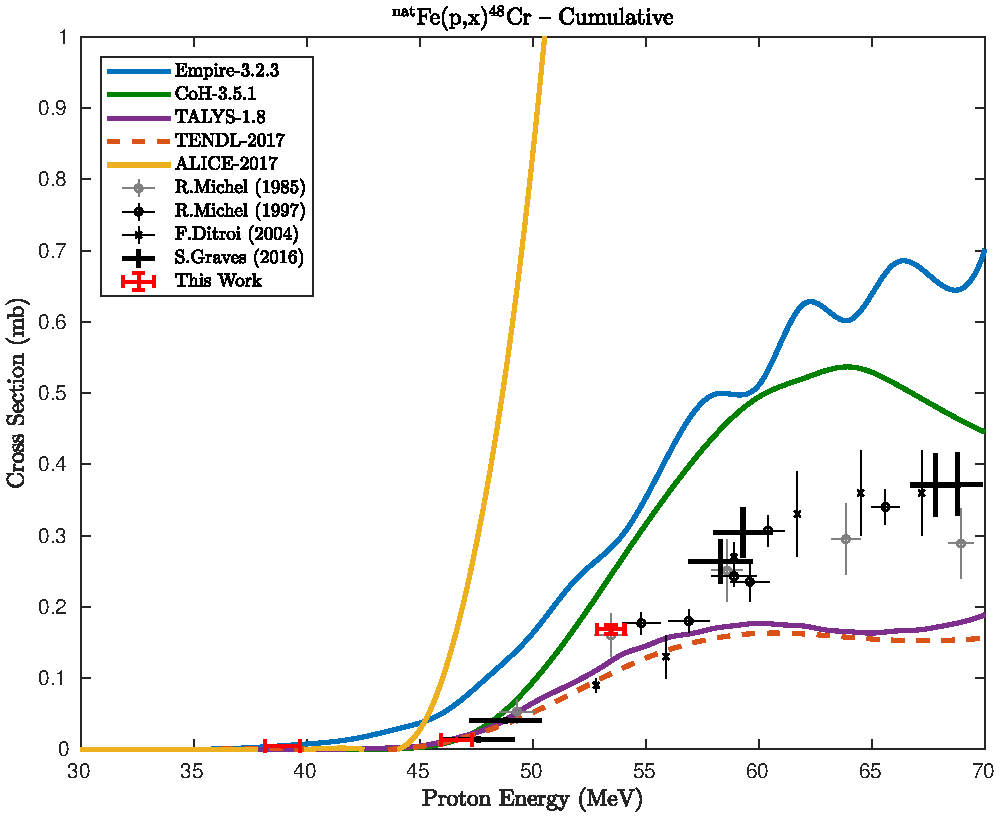
\includegraphics[width=0.49\textwidth]{./figures/48Cr.pdf}
 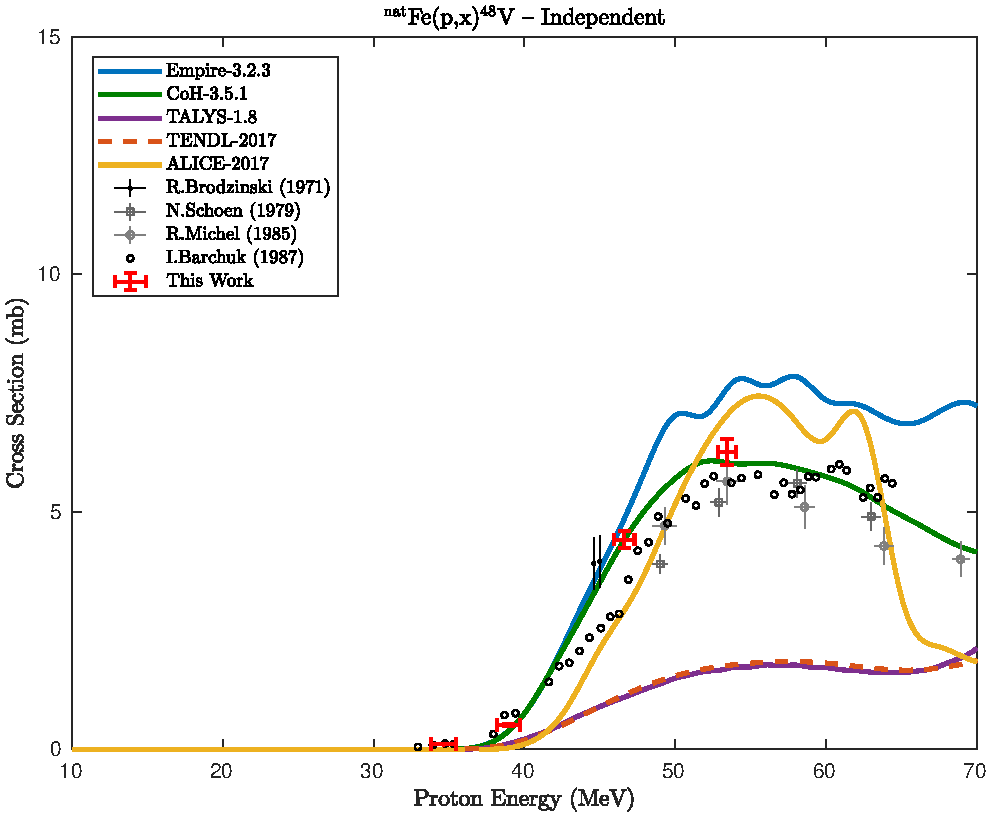
\includegraphics[width=0.49\textwidth]{./figures/48V_ind.pdf}
 
%  \\
 
 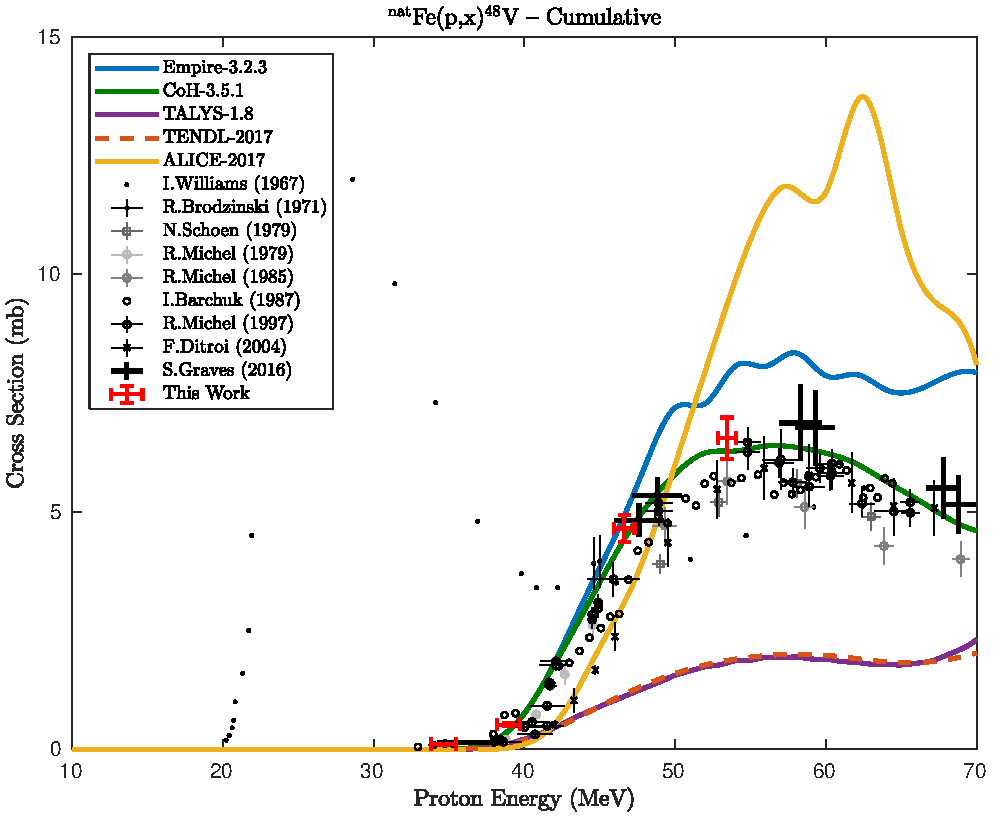
\includegraphics[width=0.49\textwidth]{./figures/48V_cum.pdf}
 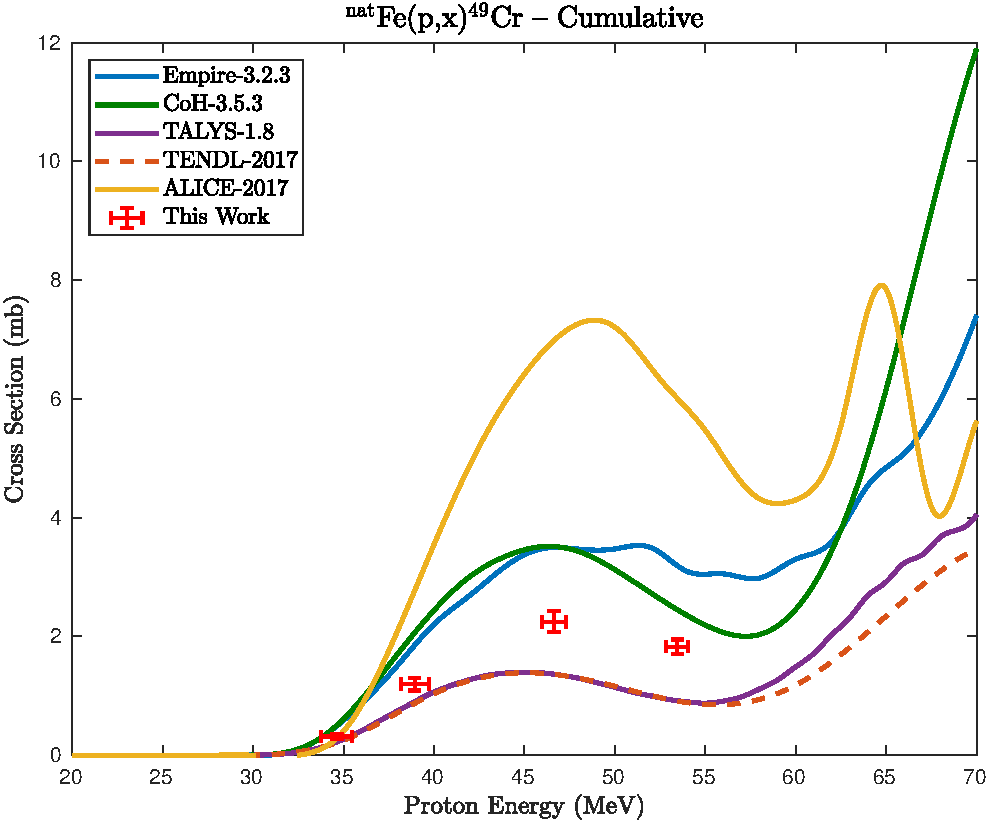
\includegraphics[width=0.49\textwidth]{./figures/49Cr.pdf}
 
%  \medskip
 
%  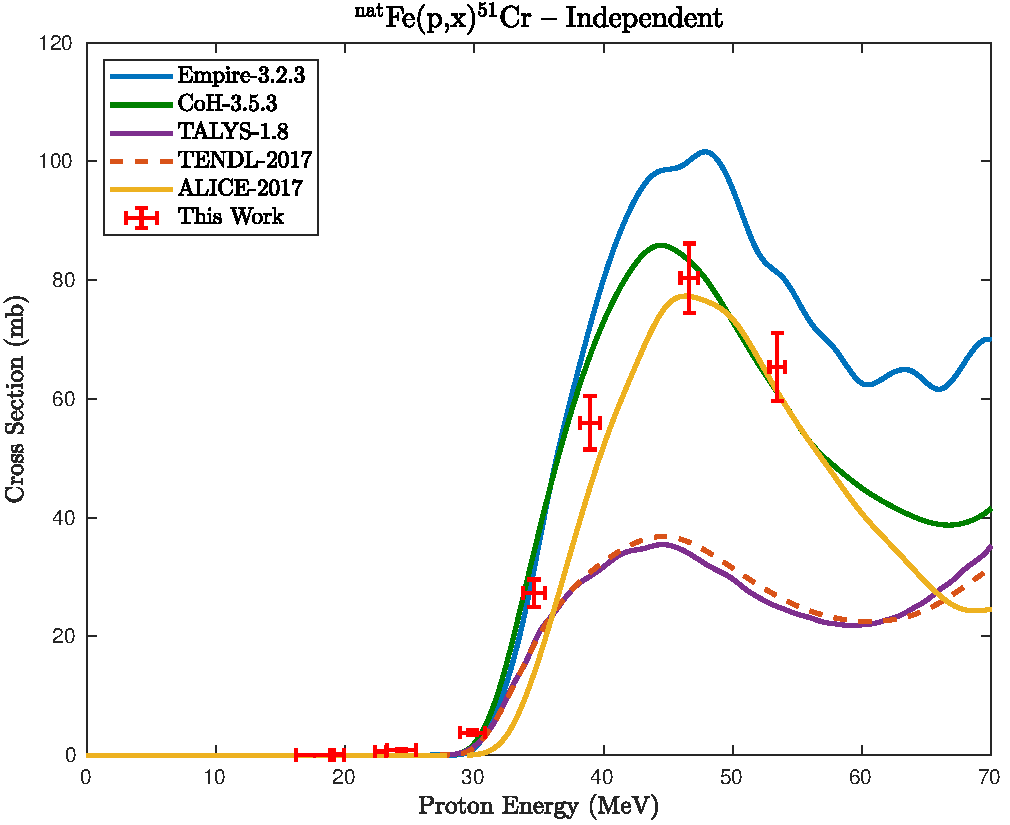
\includegraphics[width=0.49\textwidth]{./figures/51Cr_ind.pdf}
 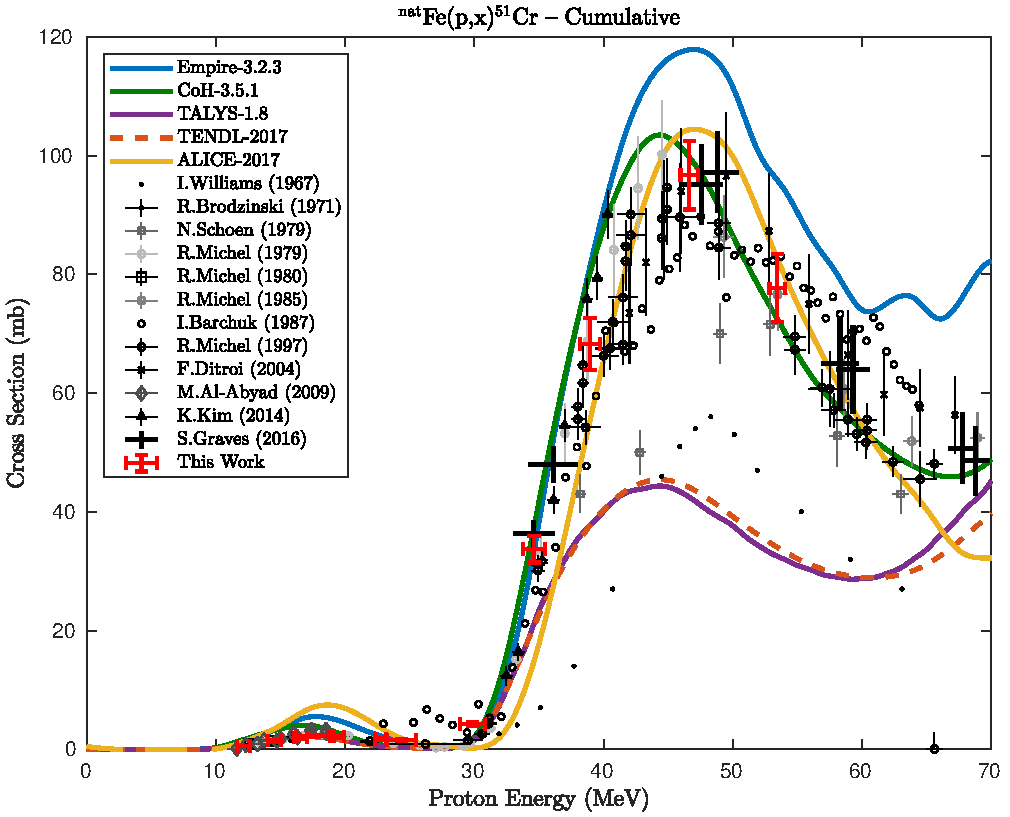
\includegraphics[width=0.49\textwidth]{./figures/51Cr_cum.pdf}
 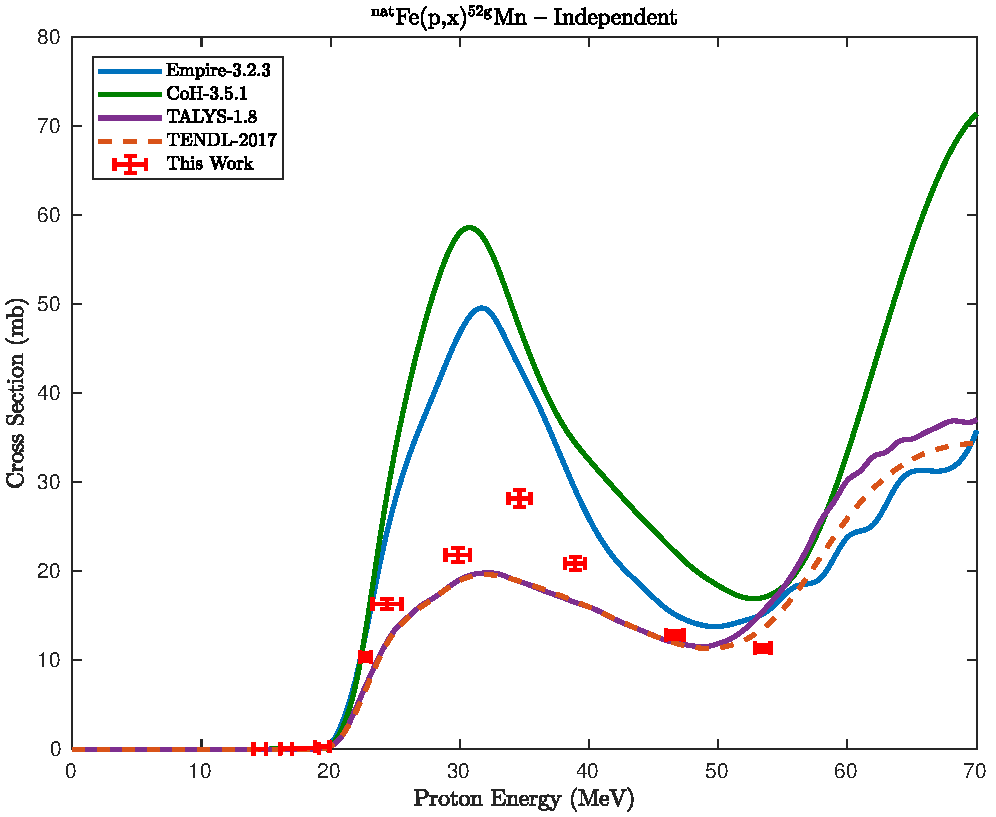
\includegraphics[width=0.49\textwidth]{./figures/52gMn.pdf}

\vspace{-20pt} 
\end{figure*}





% \begin{figure*}
%     \sloppy
%     \centering
%     \vspace{-8pt}\subfloat{
%         \centering
% %         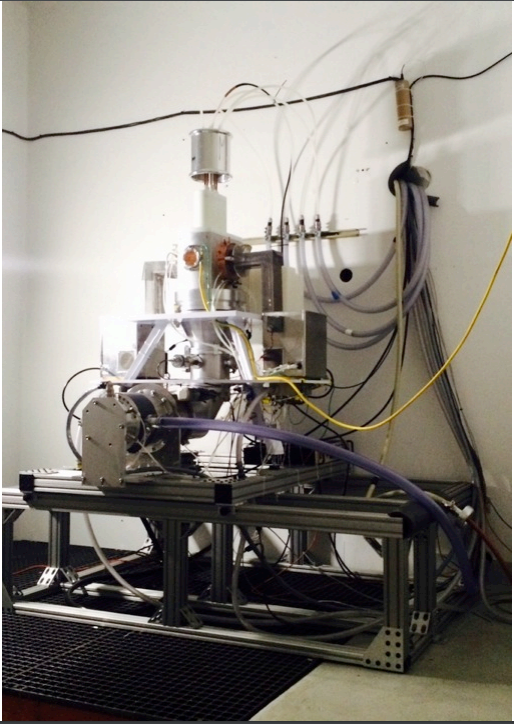
\includegraphics[width=\columnwidth]{./figures/Capture.PNG}
%         \subfigimg[width=0.49\textwidth]{}{./figures/48Cr.pdf}{50}
% %         \caption{ Decay curve for the isomeric transition of \ce{^{115m}In}.}
% %         \refstepcounter{subfigure}
% %          \label{fig:51Cr}%
% %         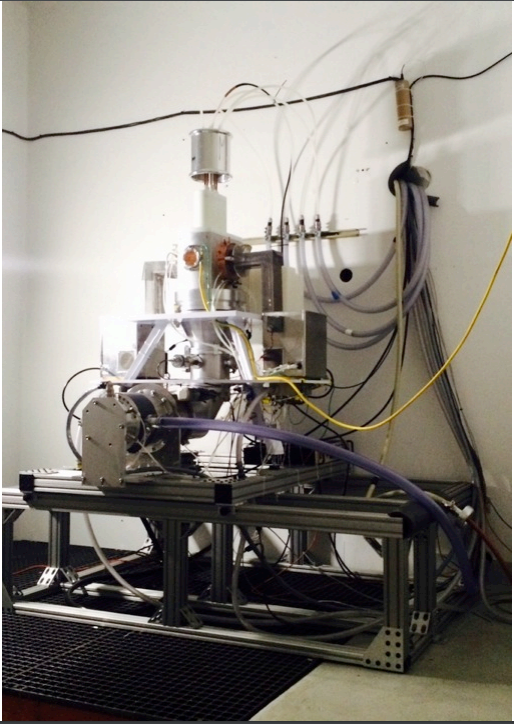
\includegraphics[width=\columnwidth]{./figures/Capture.PNG}
% %         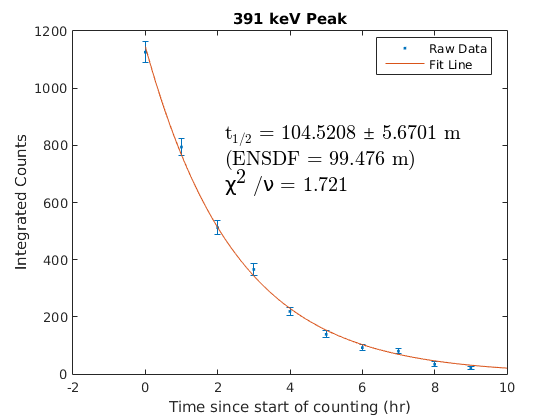
\includegraphics[scale=0.6]{./figures/391keV_curve2.png}
%         \subfigimg[width=0.49\textwidth]{}{./figures/48V_ind.pdf}{50}
% %         \caption{ Decay curve for the isomeric transition of \ce{^{113m}In}.}
% %         \refstepcounter{subfigure}
% %          \label{fig:52Mn}
% %    \hspace{-10pt}
%    }%
%     \\\vspace{-10pt}
%     \subfloat{
%         \centering
% %         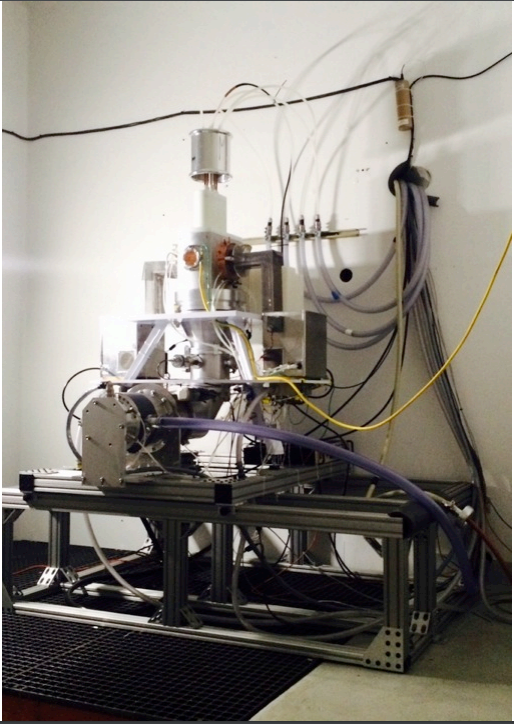
\includegraphics[width=\columnwidth]{./figures/Capture.PNG}
%         \subfigimg[width=0.49\textwidth]{}{./figures/48V_cum.pdf}{50}
% %         \caption{ Decay curve for the isomeric transition of \ce{^{115m}In}.}
% %         \refstepcounter{subfigure}
% %          \label{fig:52gMn}%
% %         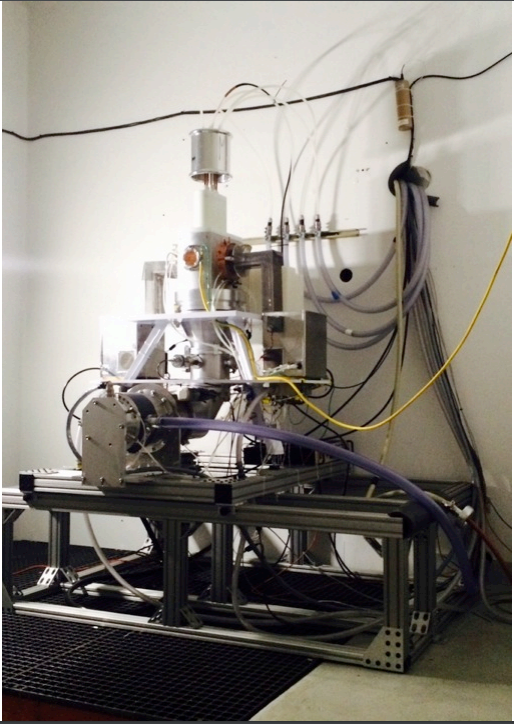
\includegraphics[width=\columnwidth]{./figures/Capture.PNG}
% %         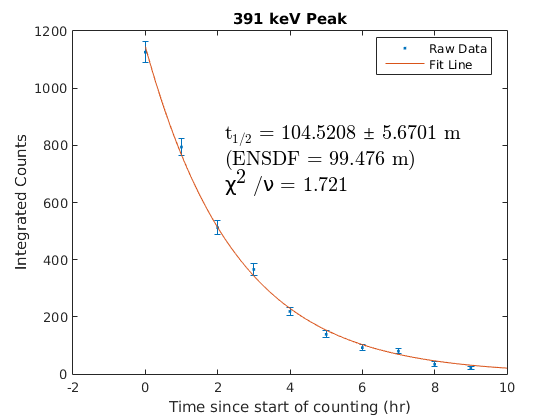
\includegraphics[scale=0.6]{./figures/391keV_curve2.png}
%         \subfigimg[width=0.49\textwidth]{}{./figures/49Cr.pdf}{50}
% %         \caption{ Decay curve for the isomeric transition of \ce{^{113m}In}.}
% %         \refstepcounter{subfigure}
% %          \label{fig:52mMn}
% %    \hspace{-10pt}
%    }%
%     \\\vspace{-10pt}
%     \subfloat{
%         \centering
% %         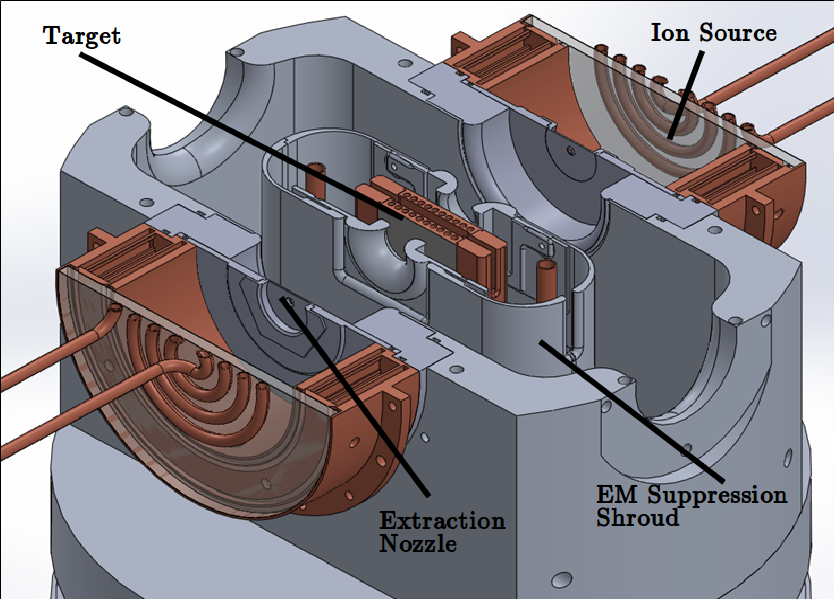
\includegraphics[width=\textwidth]{./figures/target2.png}
%         \subfigimg[width=0.49\textwidth]{}{./figures/51Cr_ind.pdf}{50}
% %         \caption{Decay curve for the $\beta^-$ decay of \ce{^{116}In}.}
%         %         \refstepcounter{subfigure}
% %          \label{fig:54Mn}
% %
% %         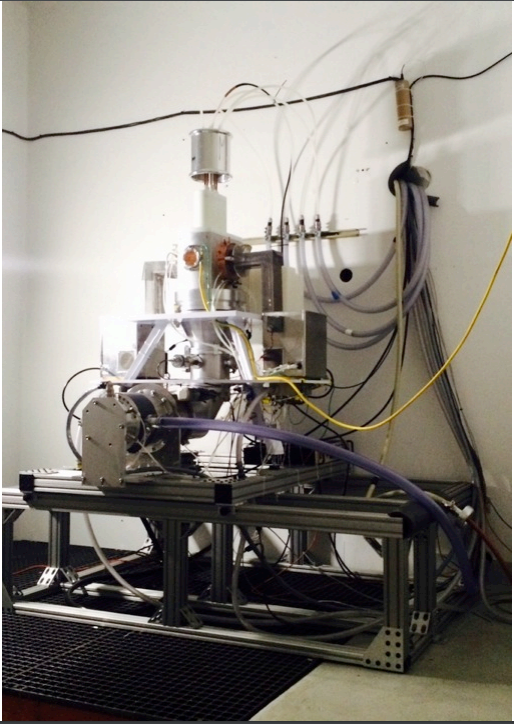
\includegraphics[width=\columnwidth]{./figures/Capture.PNG}
%         \subfigimg[width=0.49\textwidth]{}{./figures/51Cr_cum.pdf}{50}
% %         \caption{ Decay curve for the $\beta^+$ decay of \ce{^{64}Cu}.}
% %         \refstepcounter{subfigure} 
% %         \label{fig:55Co}
% %    \hspace{-10pt}
%    }%
% %     \caption{Decay curves used to verify photopeak transition assignment. (a) Decay curve for the isomeric transition of \ce{^{115m}In}, (b) decay curve for the isomeric transition of \ce{^{113m}In}, (c) decay curve for the $\beta^-$ decay of \ce{^{116}In}, and (d) decay curve for the $\beta^+$ decay of \ce{^{64}Cu}.}
% %      \phantomcaption{}\label{fig:xs_curves_p1}
% \end{figure*}

\begin{figure*}
 \centering
%  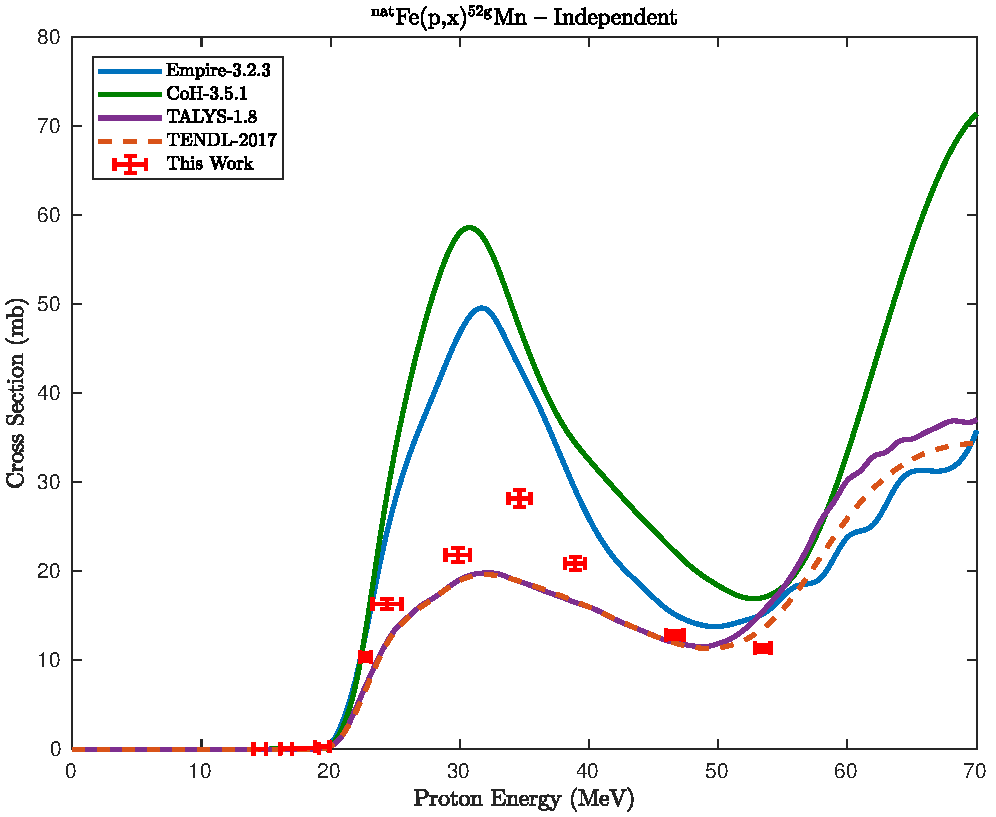
\includegraphics[width=0.49\textwidth]{./figures/52gMn.pdf}
 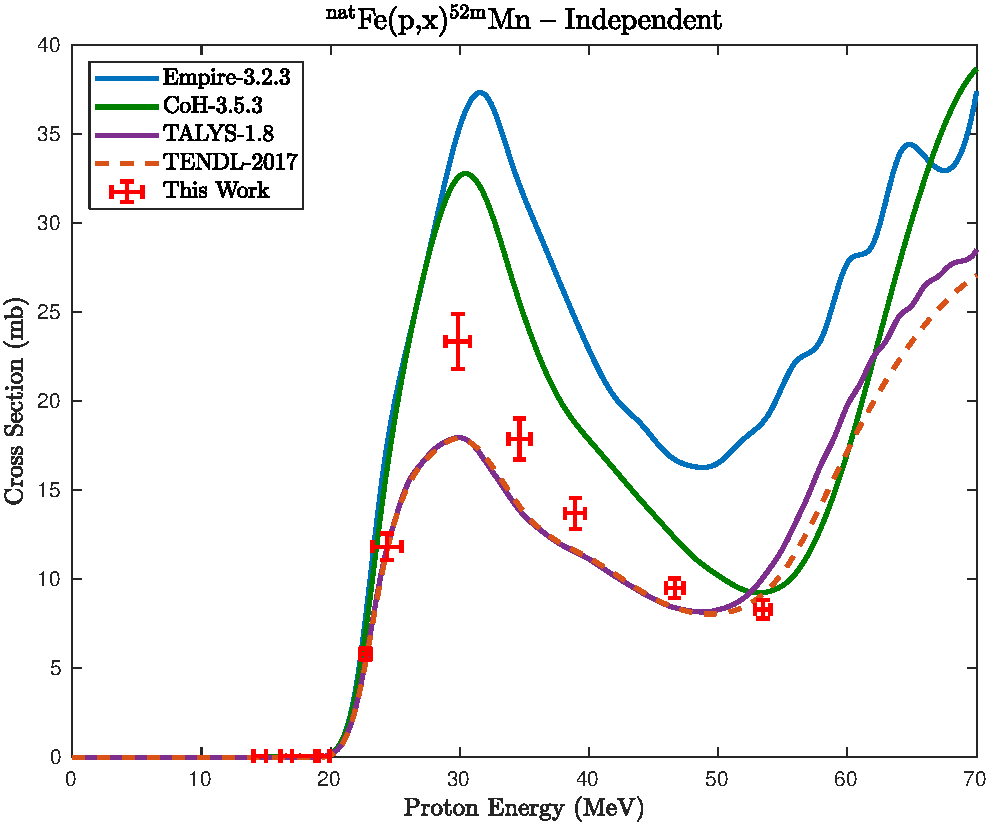
\includegraphics[width=0.49\textwidth]{./figures/52mMn.pdf}
 %  \\
 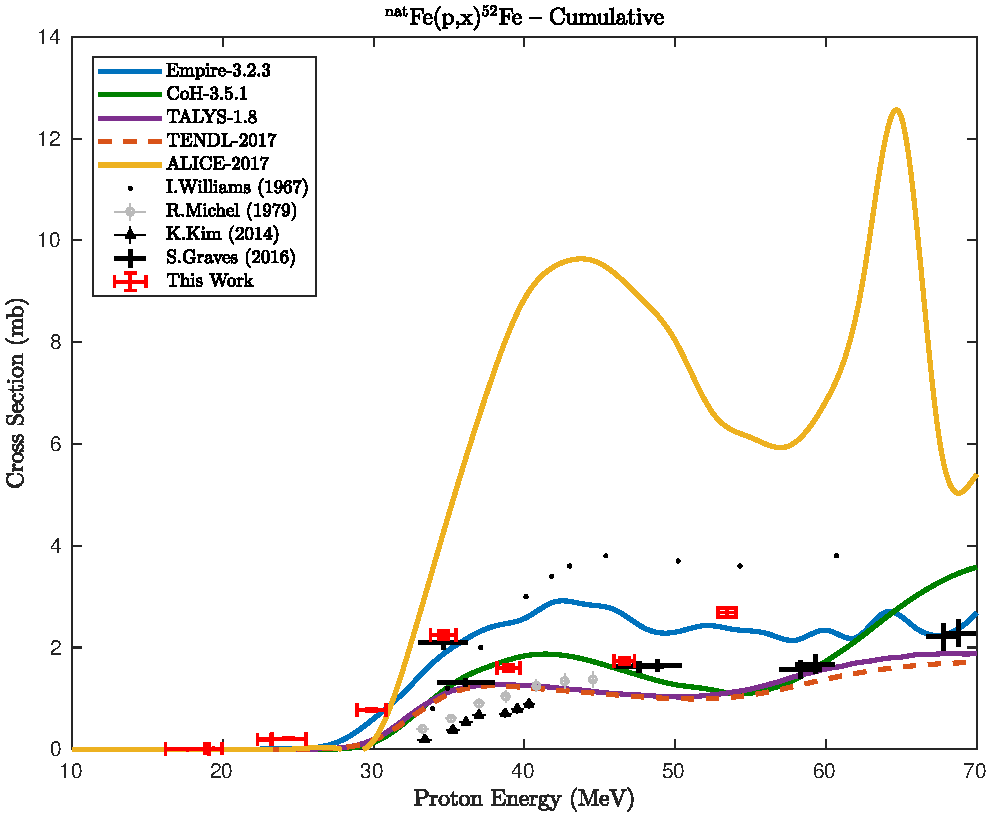
\includegraphics[width=0.49\textwidth]{./figures/52Fe.pdf}
 
%  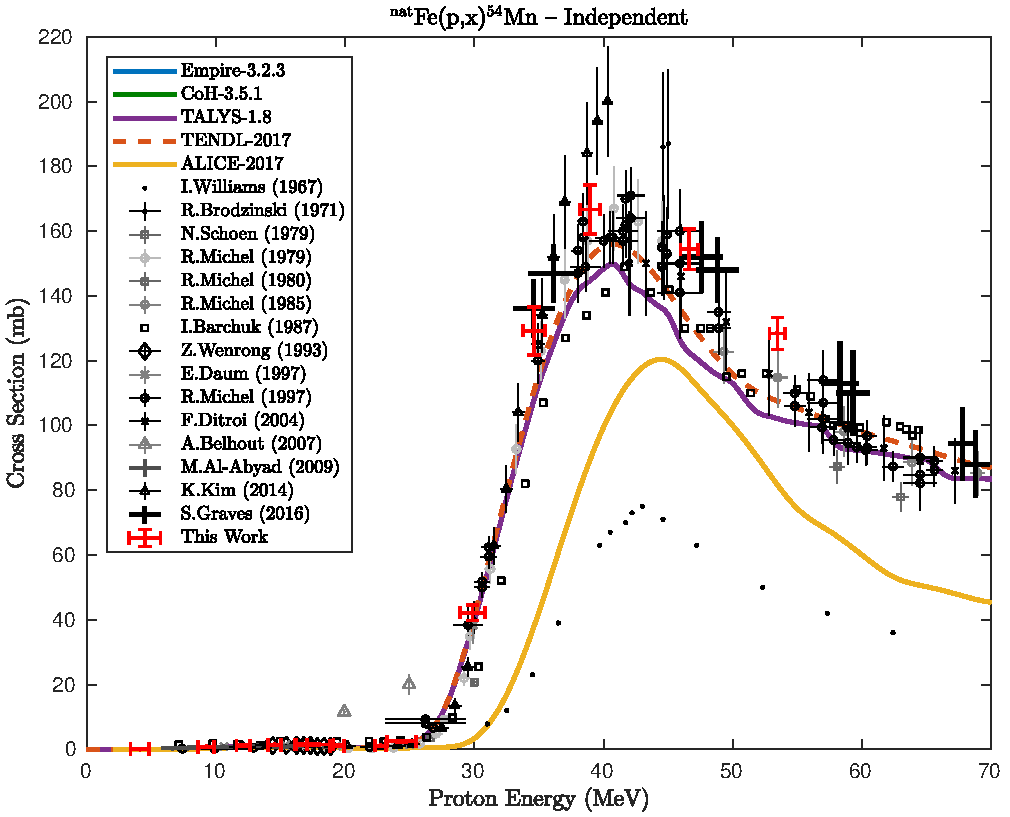
\includegraphics[width=0.49\textwidth]{./figures/54Mn.pdf}
 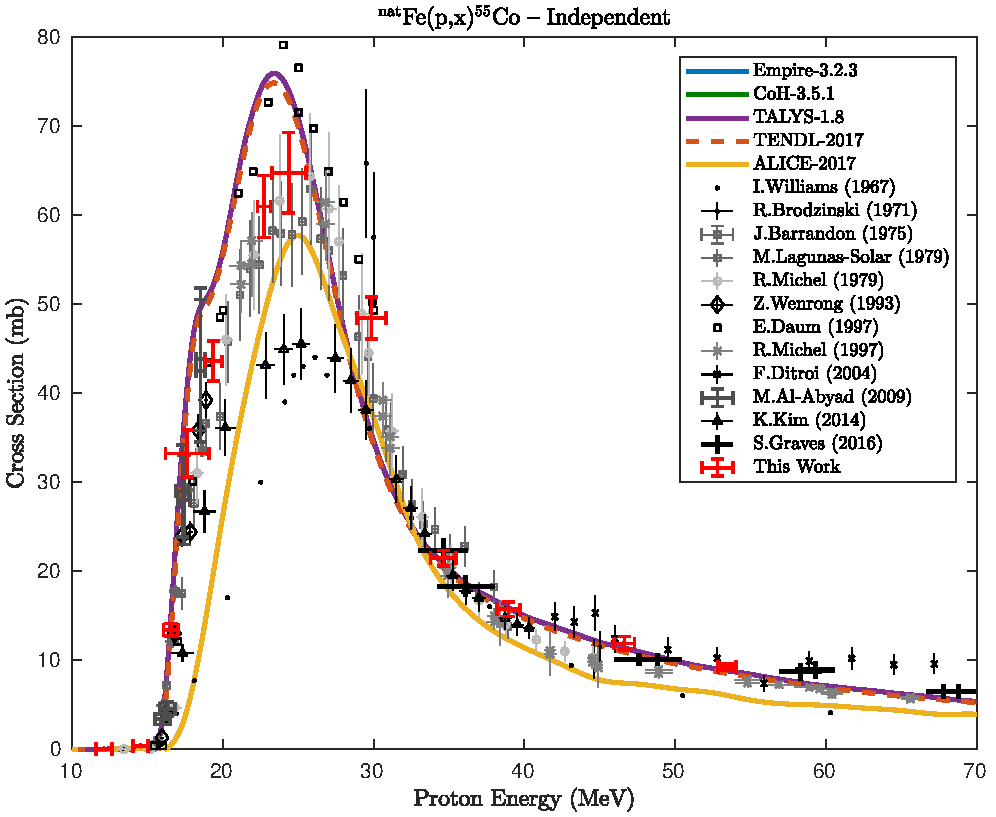
\includegraphics[width=0.49\textwidth]{./figures/55Co.pdf}
%  \medskip
 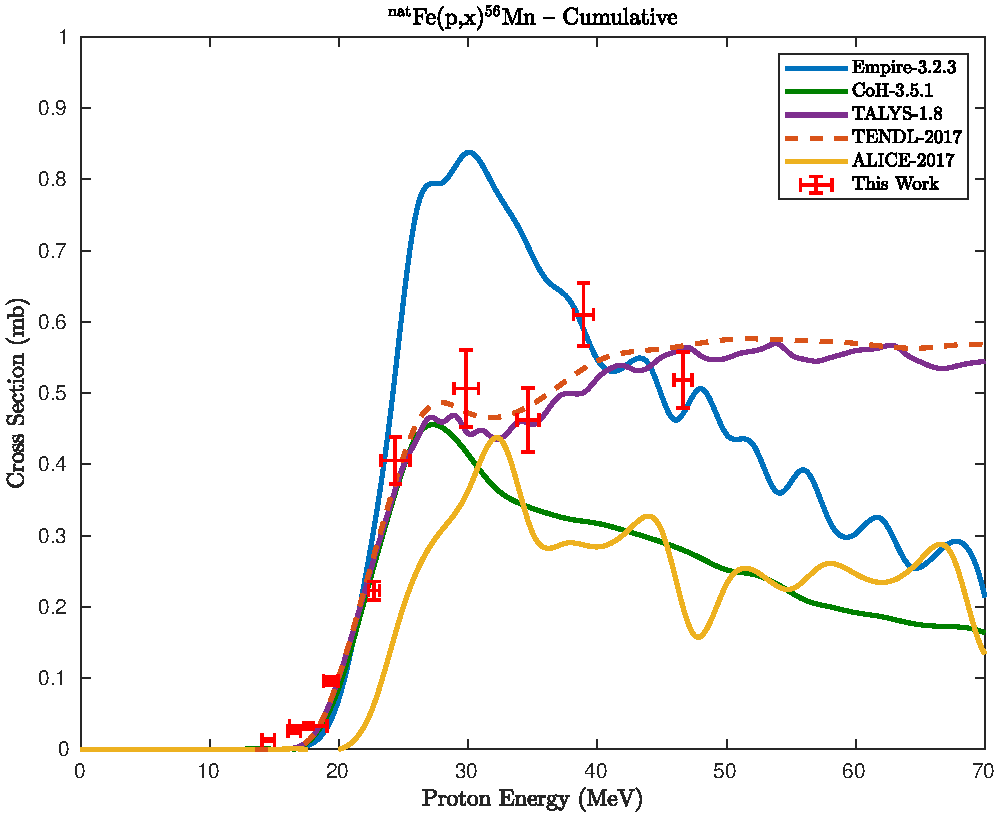
\includegraphics[width=0.49\textwidth]{./figures/56Mn.pdf}
 
 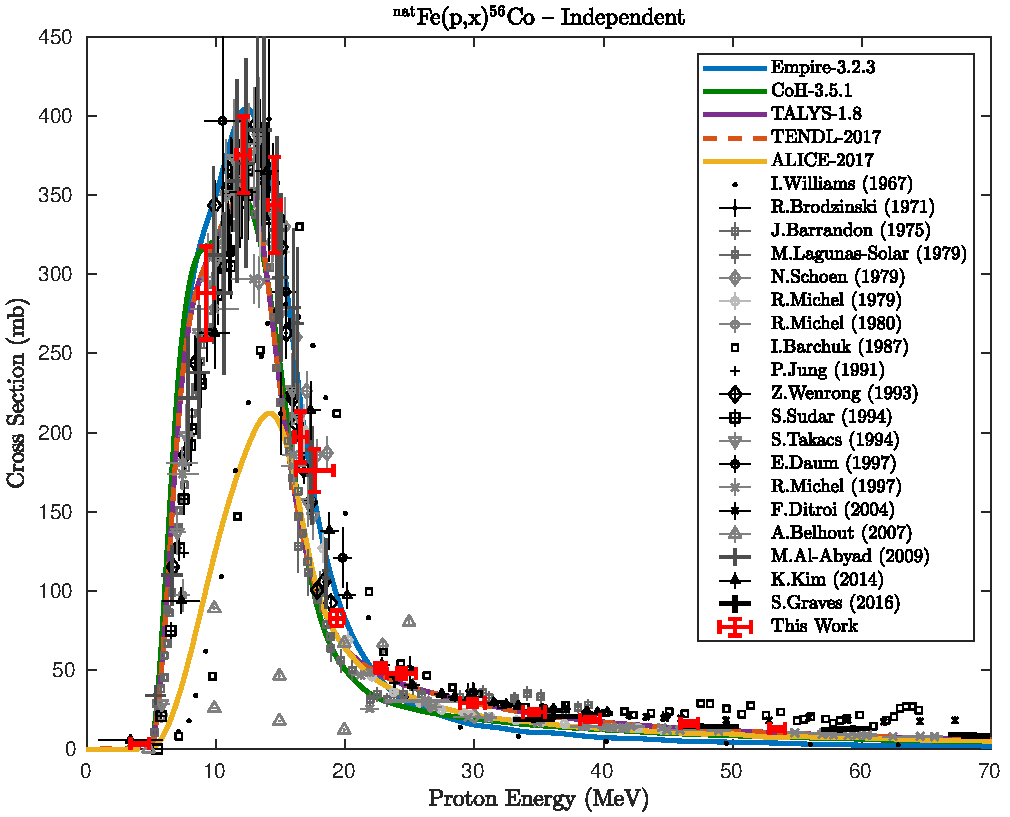
\includegraphics[width=0.49\textwidth]{./figures/56Co.pdf}
 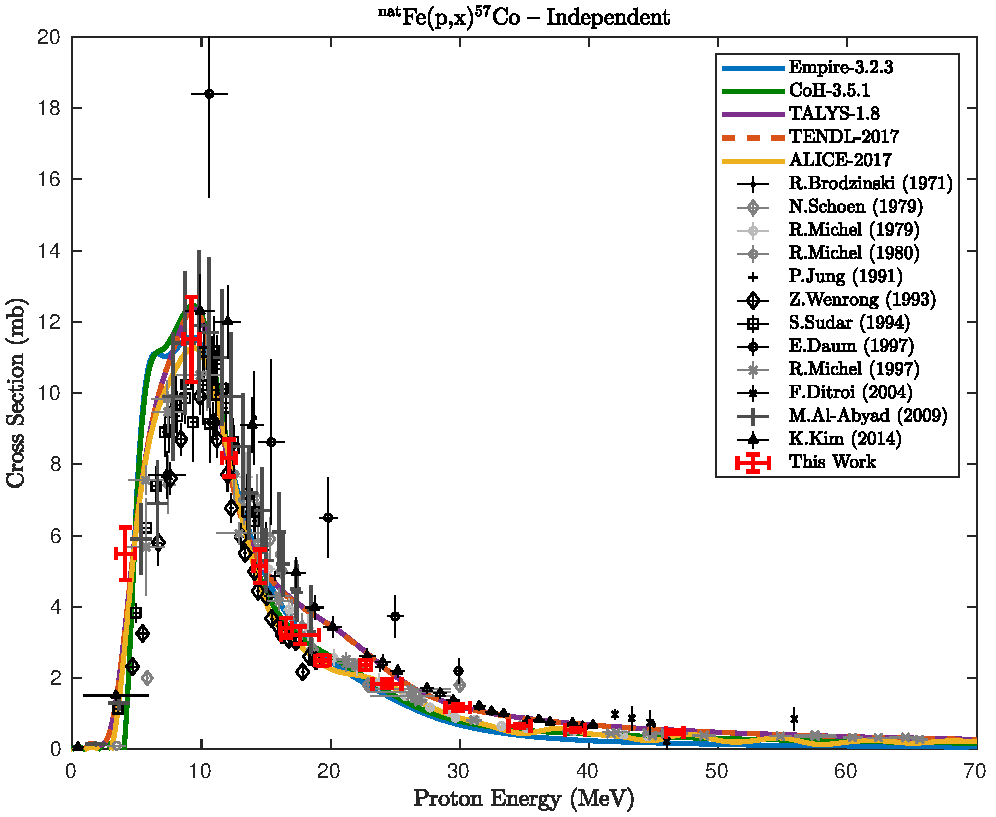
\includegraphics[width=0.49\textwidth]{./figures/57Co.pdf}

\vspace{-20pt} 
\end{figure*}



% \begin{figure*}
%     \centering
%     \vspace{-8pt}\subfloat{
%         \centering
% %         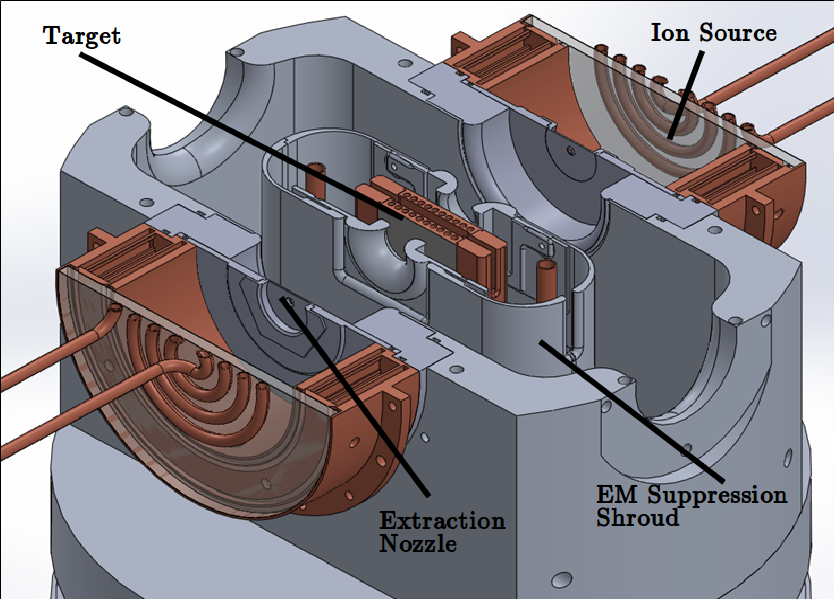
\includegraphics[width=\textwidth]{./figures/target2.png}
%         \subfigimg[width=0.49\textwidth]{}{./figures/52gMn.pdf}{50}
% %         \caption{Decay curve for the $\beta^-$ decay of \ce{^{116}In}.}
%         %         \refstepcounter{subfigure}
% %          \label{fig:56Ni}
% %
% %         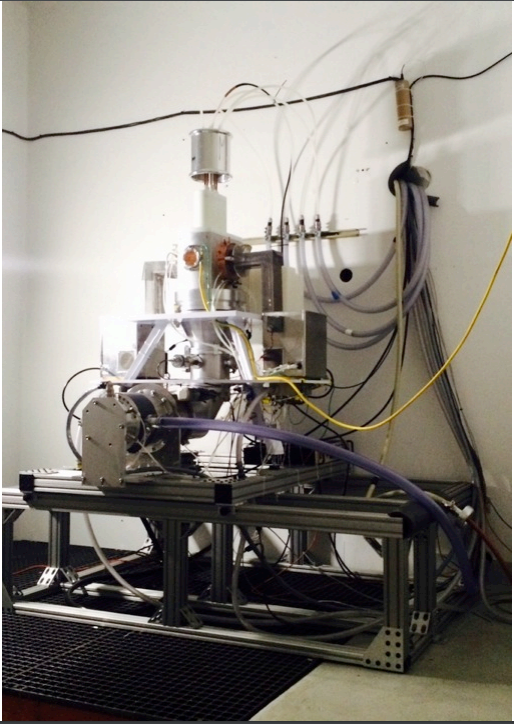
\includegraphics[width=\columnwidth]{./figures/Capture.PNG}
%         \subfigimg[width=0.49\textwidth]{}{./figures/52Fe.pdf}{50}
% %         \caption{ Decay curve for the $\beta^+$ decay of \ce{^{64}Cu}.}
% %         \refstepcounter{subfigure}
% %         \label{fig:57Co}
% %    \hspace{-10pt}
%    }%
%     \\\vspace{-10pt}
%     \subfloat{
%         \centering
% %         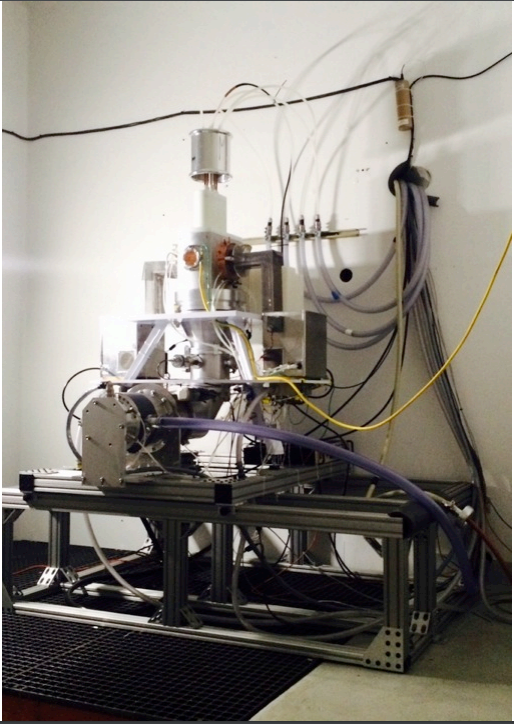
\includegraphics[width=\columnwidth]{./figures/Capture.PNG}
%         \subfigimg[width=0.49\textwidth]{}{./figures/54Mn.pdf}{50}
% %         \caption{ Decay curve for the isomeric transition of \ce{^{115m}In}.}
% %         \refstepcounter{subfigure}
% %          \label{fig:57Ni}%
% %         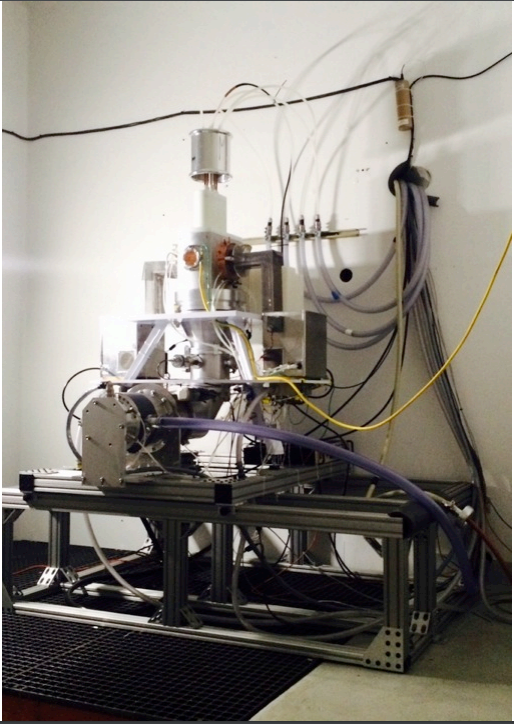
\includegraphics[width=\columnwidth]{./figures/Capture.PNG}
% %         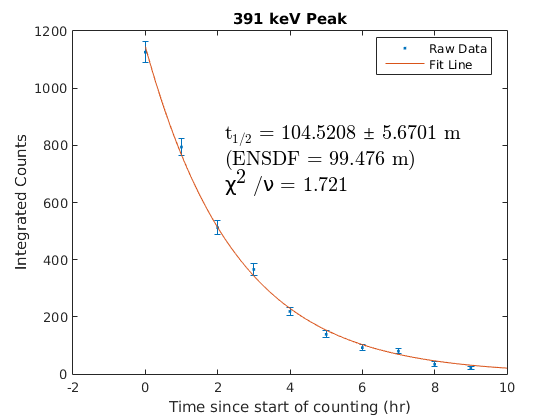
\includegraphics[scale=0.6]{./figures/391keV_curve2.png}
%         \subfigimg[width=0.49\textwidth]{}{./figures/55Co.pdf}{50}
% %         \caption{ Decay curve for the isomeric transition of \ce{^{113m}In}.}
% %         \refstepcounter{subfigure}
% %          \label{fig:58Co}
% %    \hspace{-10pt}
%    }%
%     \\\vspace{-10pt}
%     \subfloat{
%         \centering
% %         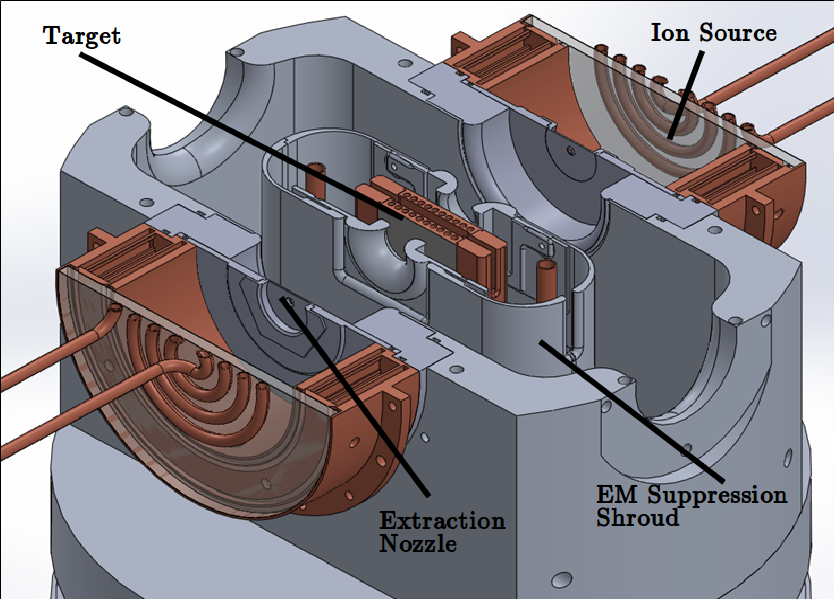
\includegraphics[width=\textwidth]{./figures/target2.png}
%         \subfigimg[width=0.49\textwidth]{}{./figures/56Mn.pdf}{50}
% %         \caption{Decay curve for the $\beta^-$ decay of \ce{^{116}In}.}
%         %         \refstepcounter{subfigure}
% %          \label{fig:58gCo}
% %
% %         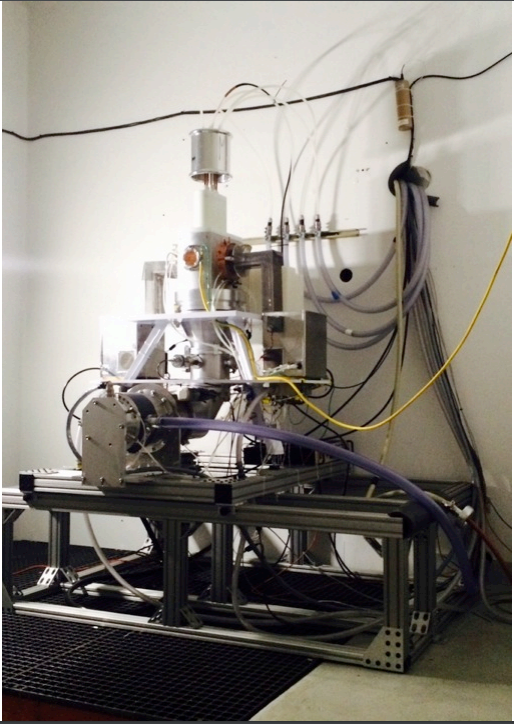
\includegraphics[width=\columnwidth]{./figures/Capture.PNG}
%         \subfigimg[width=0.49\textwidth]{}{./figures/56Co.pdf}{50}
% %         \caption{ Decay curve for the $\beta^+$ decay of \ce{^{64}Cu}.}
% %         \refstepcounter{subfigure}
% %         \label{fig:58mCo}
% %    \hspace{-10pt}
%    }%
% %     \caption{Decay curves used to verify photopeak transition assignment. (a) Decay curve for the isomeric transition of \ce{^{115m}In}, (b) decay curve for the isomeric transition of \ce{^{113m}In}, (c) decay curve for the $\beta^-$ decay of \ce{^{116}In}, and (d) decay curve for the $\beta^+$ decay of \ce{^{64}Cu}.}
% %      \phantomcaption{}\label{fig:xs_curves_p2}
% \end{figure*}

\begin{figure*}
 \centering
%  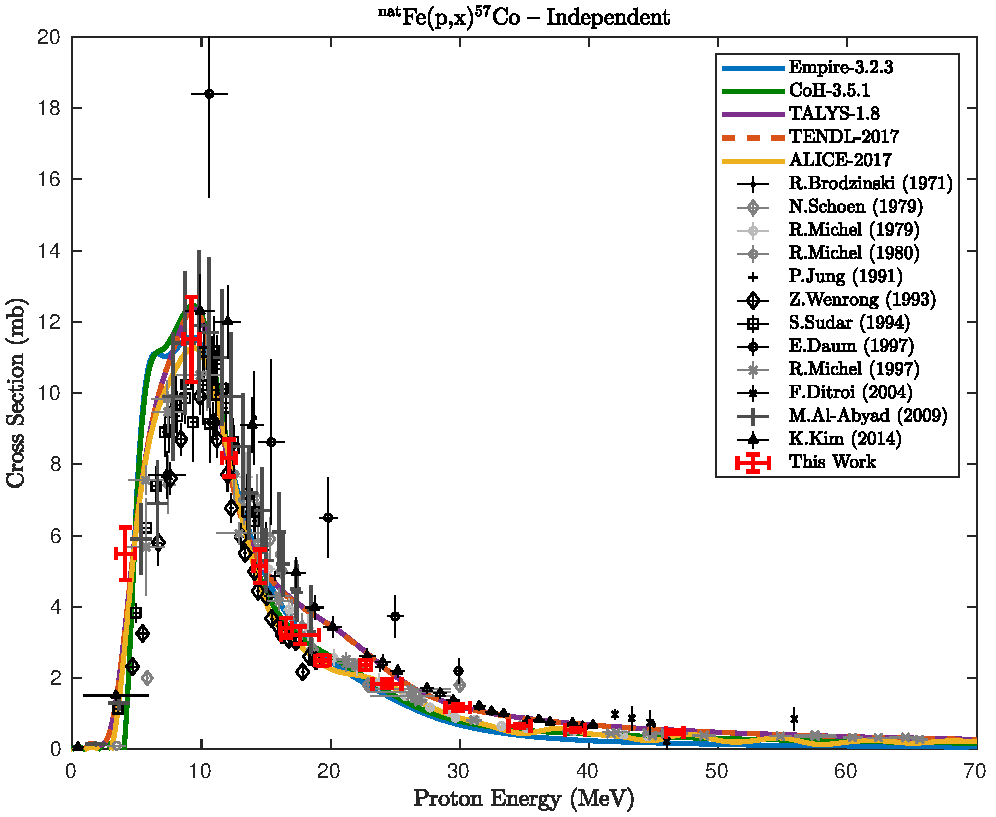
\includegraphics[width=0.49\textwidth]{./figures/57Co.pdf}
 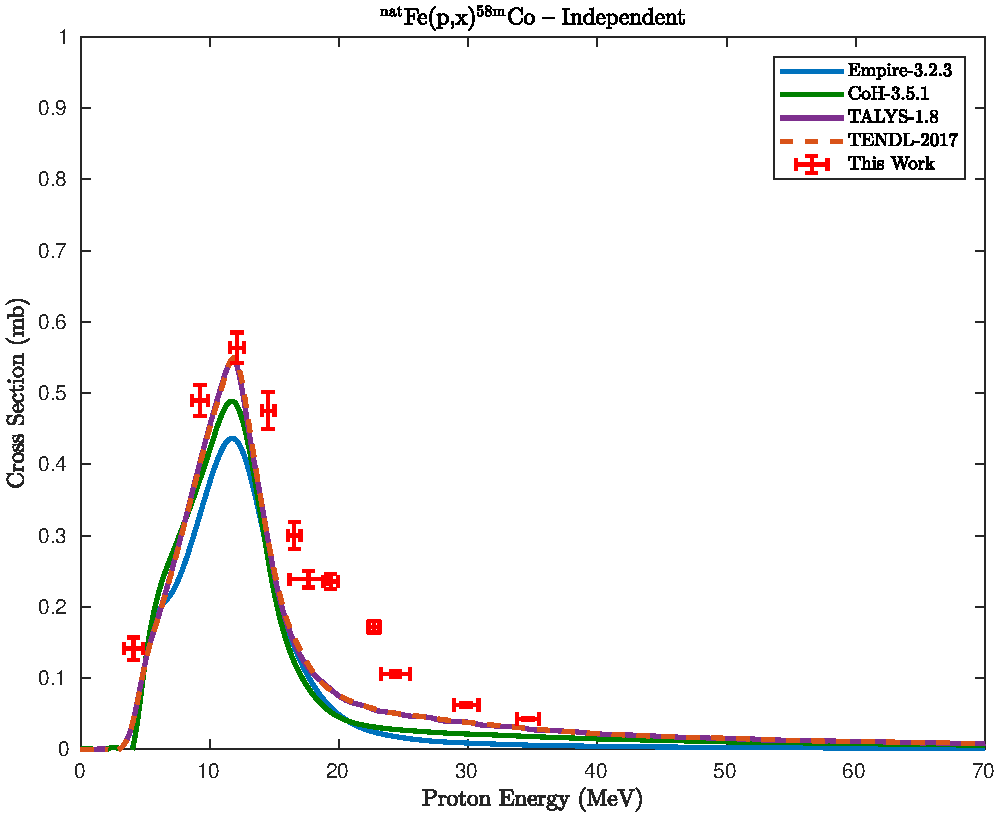
\includegraphics[width=0.49\textwidth]{./figures/58mCo.pdf}
%  \\
 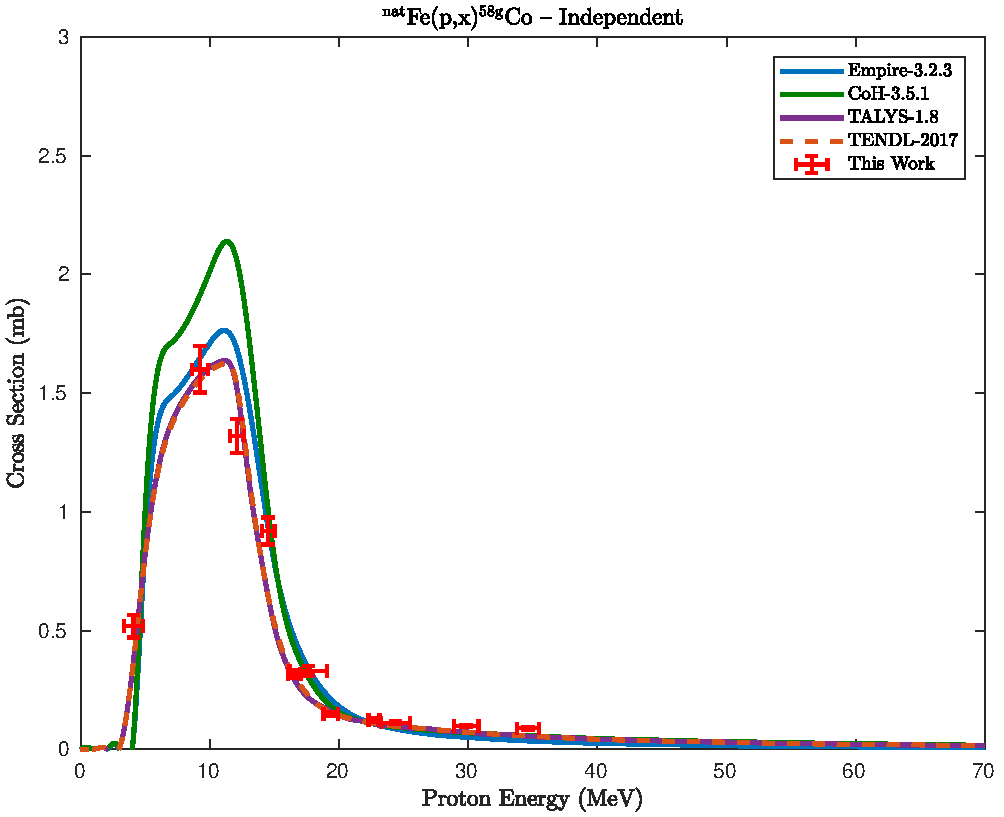
\includegraphics[width=0.49\textwidth]{./figures/58gCo.pdf}
 
 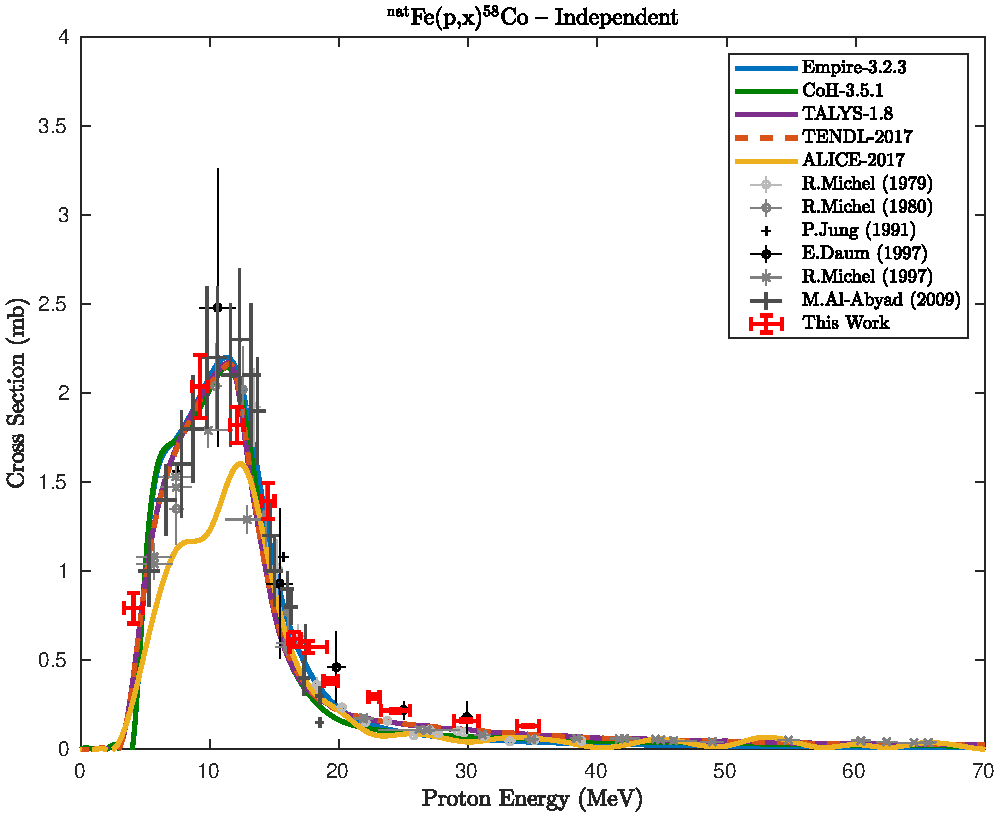
\includegraphics[width=0.49\textwidth]{./figures/58Co.pdf}
%  \medskip
 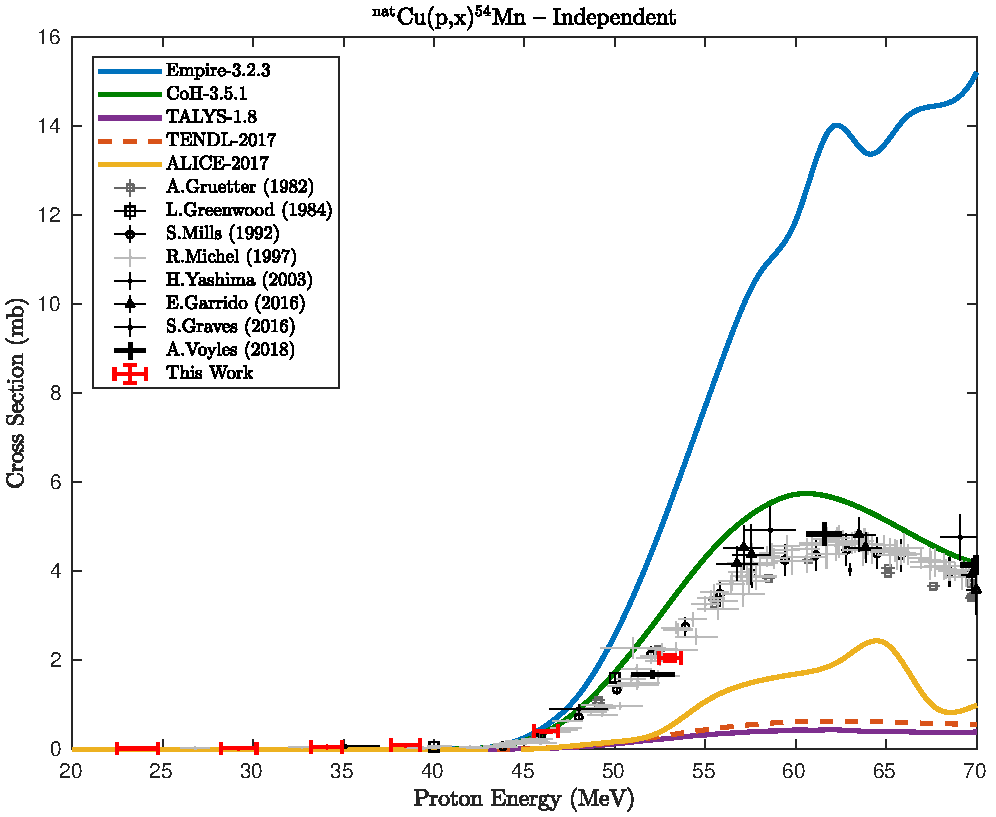
\includegraphics[width=0.49\textwidth]{./figures/54MnCu.pdf}
 
 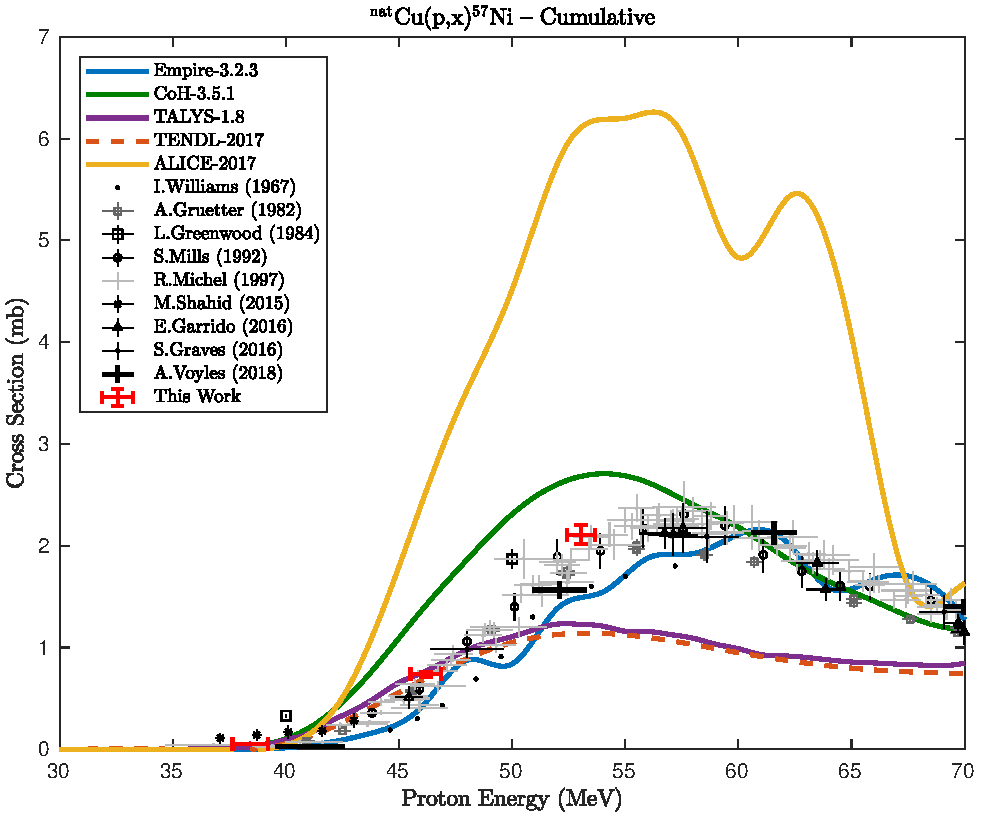
\includegraphics[width=0.49\textwidth]{./figures/57Ni.pdf}
 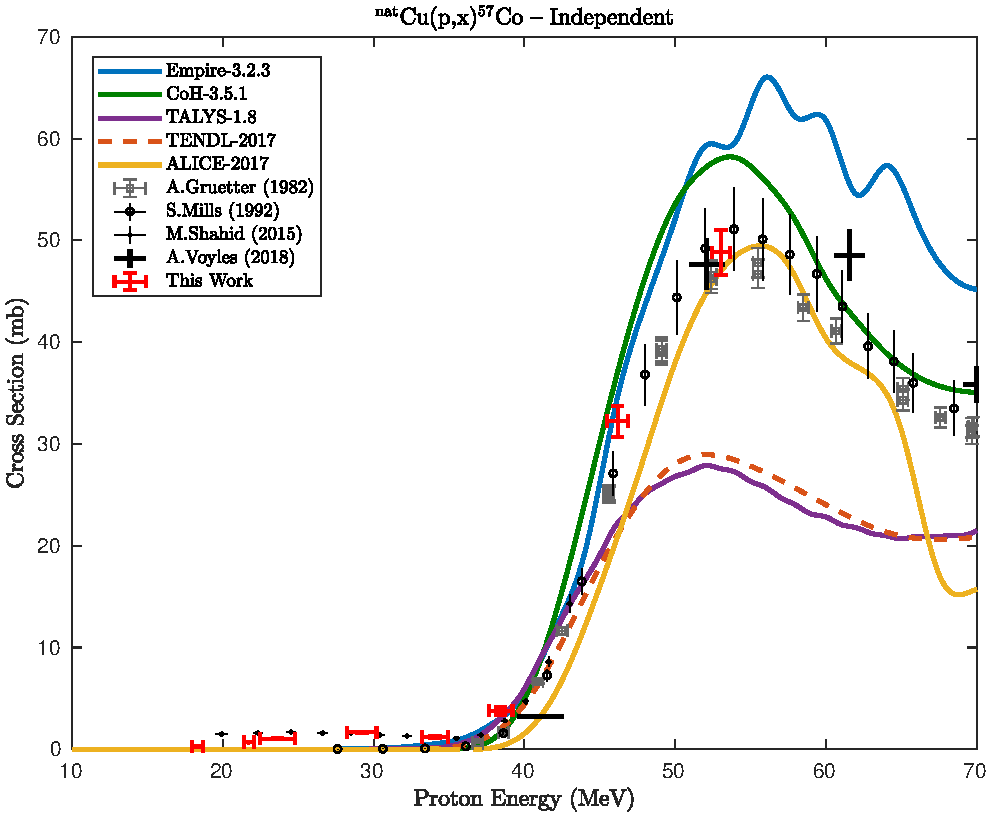
\includegraphics[width=0.49\textwidth]{./figures/57Co_ind.pdf}

\vspace{-20pt} 
\end{figure*}

% \begin{figure*}
%     \centering
%     \vspace{-8pt}\subfloat{
%         \centering
% %         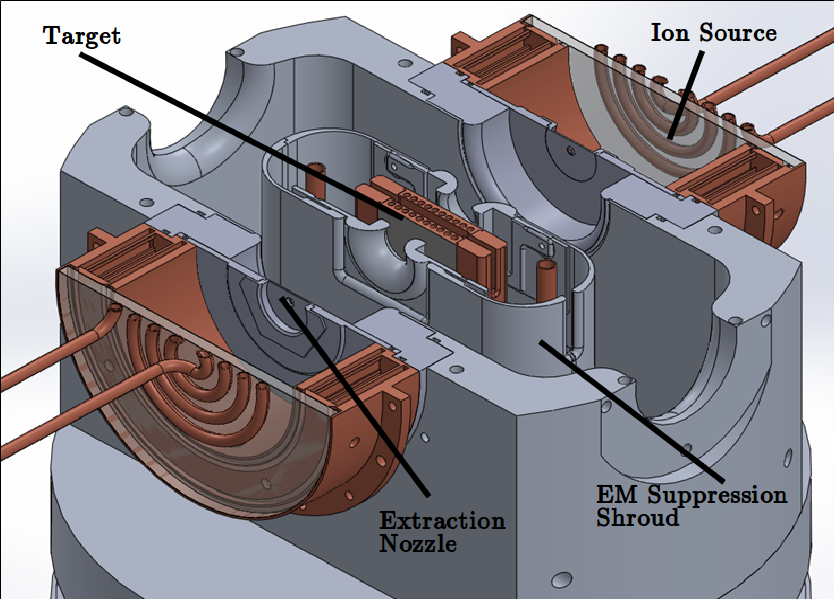
\includegraphics[width=\textwidth]{./figures/target2.png}
%         \subfigimg[width=0.49\textwidth]{}{./figures/57Co.pdf}{50}
% %         \caption{Decay curve for the $\beta^-$ decay of \ce{^{116}In}.}
%         %         \refstepcounter{subfigure}
% %          \label{fig:59Fe}
% %
% %         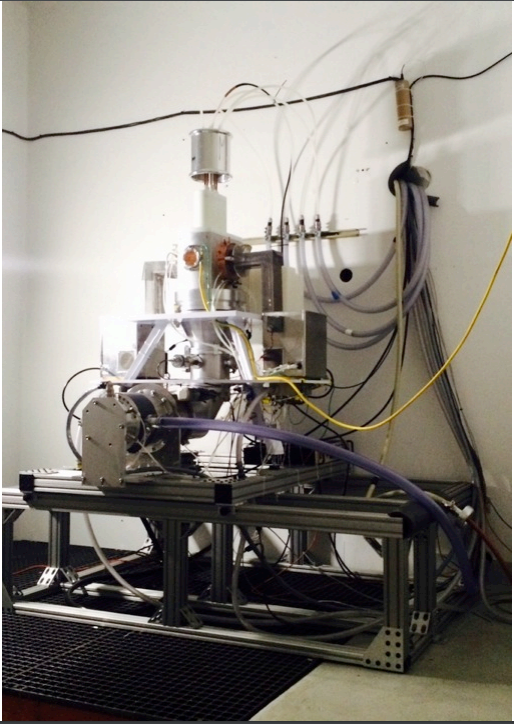
\includegraphics[width=\columnwidth]{./figures/Capture.PNG}
%         \subfigimg[width=0.49\textwidth]{}{./figures/58mCo.pdf}{50}
% %         \caption{ Decay curve for the $\beta^+$ decay of \ce{^{64}Cu}.}
% %         \refstepcounter{subfigure} 
% %         \label{fig:60Co}
% %    \hspace{-10pt}
%    }%
%     \\\vspace{-10pt}
%     \subfloat{
%         \centering
% %         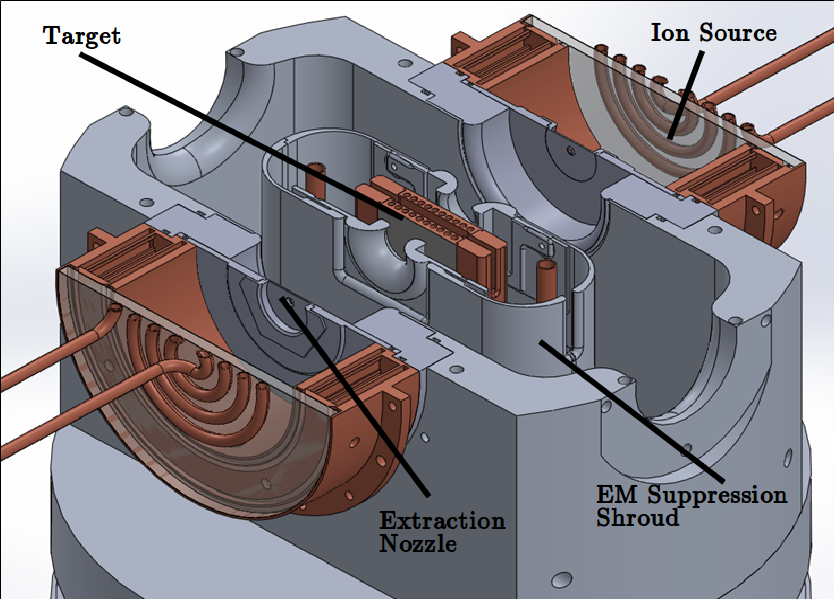
\includegraphics[width=\textwidth]{./figures/target2.png}
%         \subfigimg[width=0.49\textwidth]{}{./figures/58gCo.pdf}{50}
% %         \caption{Decay curve for the $\beta^-$ decay of \ce{^{116}In}.}
%         %         \refstepcounter{subfigure}
% %          \label{fig:61Cu}
% %
% %         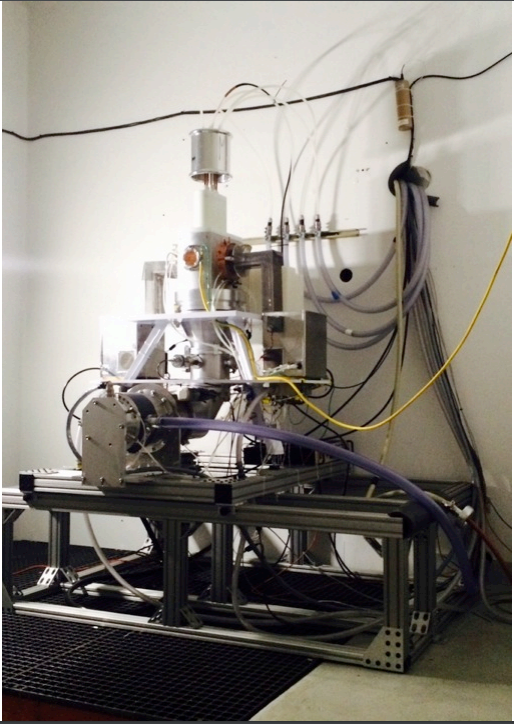
\includegraphics[width=\columnwidth]{./figures/Capture.PNG}
%         \subfigimg[width=0.49\textwidth]{}{./figures/58Co.pdf}{50}
% %         \caption{ Decay curve for the $\beta^+$ decay of \ce{^{64}Cu}.}
% %         \refstepcounter{subfigure}
% %         \label{fig:64Cu}
% %    \hspace{-10pt}
%    }%
%     \\\vspace{-10pt}
%     \subfloat{
%         \centering
% %         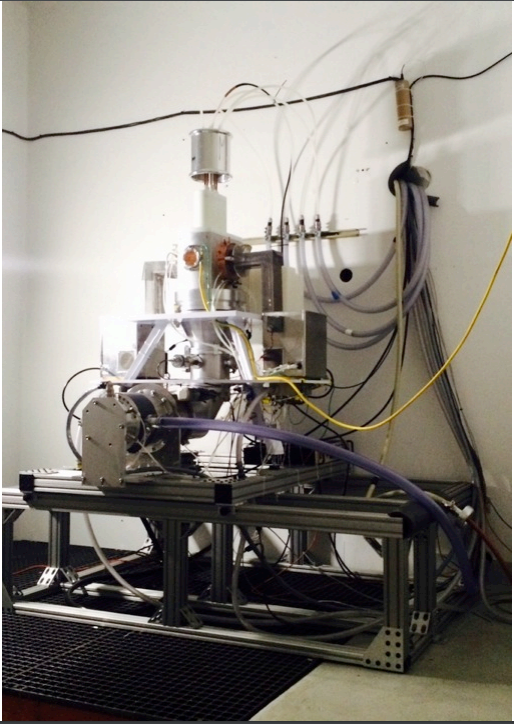
\includegraphics[width=\columnwidth]{./figures/Capture.PNG}
%         \subfigimg[width=0.49\textwidth]{}{./figures/54MnCu.pdf}{50}
% %         \caption{ Decay curve for the isomeric transition of \ce{^{115m}In}.}
% %         \refstepcounter{subfigure}
% %          \label{fig:82mRb}%
% %         \includegraphics[width=\columnwidth]{./figures/Capture.PNG}
% %         \includegraphics[scale=0.6]{./figures/391keV_curve2.png}
%         \subfigimg[width=0.49\textwidth]{}{./figures/57Ni.pdf}{50}
% %         \caption{ Decay curve for the isomeric transition of \ce{^{113m}In}.}
% %         \refstepcounter{subfigure}
% %          \label{fig:83Sr}
% %    \hspace{-10pt}
%    }%
% %    \vspace{-5pt}
% %     \caption{Decay curves used to verify photopeak transition assignment. (a) Decay curve for the isomeric transition of \ce{^{115m}In}, (b) decay curve for the isomeric transition of \ce{^{113m}In}, (c) decay curve for the $\beta^-$ decay of \ce{^{116}In}, and (d) decay curve for the $\beta^+$ decay of \ce{^{64}Cu}.}
% %      \phantomcaption{}\label{fig:xs_curves_p3}
%      \vspace{-5pt}
% \end{figure*}

\begin{figure*}
 \centering
%  \includegraphics[width=0.49\textwidth]{./figures/57Co_ind.pdf}
 \includegraphics[width=0.49\textwidth]{./figures/57Co_cum.pdf}
%  \\
 \includegraphics[width=0.49\textwidth]{./figures/60Co.pdf}
 
 \includegraphics[width=0.49\textwidth]{./figures/60Cu.pdf}
%  \medskip
 \includegraphics[width=0.49\textwidth]{./figures/61Co.pdf}
 
 \includegraphics[width=0.49\textwidth]{./figures/61Cu.pdf}
%  \includegraphics[width=0.49\textwidth]{./figures/64Cu.pdf}
 \includegraphics[width=0.49\textwidth]{./figures/43K.pdf}


\vspace{-20pt} 
\end{figure*}


% \begin{figure*}
%     \centering
%     \vspace{-8pt}\subfloat{
%         \centering
% %         \includegraphics[width=\textwidth]{./figures/target2.png}
%         \subfigimg[width=0.49\textwidth]{}{./figures/57Co_ind.pdf}{50}
% %         \caption{Decay curve for the $\beta^-$ decay of \ce{^{116}In}.}
%         %         \refstepcounter{subfigure}
% %          \label{fig:85Y}
% %
% %         \includegraphics[width=\columnwidth]{./figures/Capture.PNG}
%         \subfigimg[width=0.49\textwidth]{}{./figures/57Co_cum.pdf}{50}
% %         \caption{ Decay curve for the $\beta^+$ decay of \ce{^{64}Cu}.}
% %         \refstepcounter{subfigure} 
% %         \label{fig:85gY}
% %    \hspace{-10pt}
%    }%
%     \\\vspace{-10pt}
%     \subfloat{
%         \centering
% %         \includegraphics[width=\textwidth]{./figures/target2.png}
%         \subfigimg[width=0.49\textwidth]{}{./figures/60Co.pdf}{50}
% %         \caption{Decay curve for the $\beta^-$ decay of \ce{^{116}In}.}
%         %         \refstepcounter{subfigure}
% %          \label{fig:85mY}
% %    }
% %      \subfloat{
% %         \centering
% % %         \includegraphics[width=\textwidth]{./figures/target2.png}
% %         \subfigimg[width=0.49\textwidth]{}{./figures/86Y.pdf}{50}
% % %         \caption{Decay curve for the $\beta^-$ decay of \ce{^{116}In}.}
% %         %         \refstepcounter{subfigure}
% %          \label{fig:86Y}
% %    }
% %     \\
% %     \subfloat{
% %         \centering
% %         \includegraphics[width=\columnwidth]{./figures/Capture.PNG}
%         \subfigimg[width=0.49\textwidth]{}{./figures/60Cu.pdf}{50}
% %         \caption{ Decay curve for the $\beta^+$ decay of \ce{^{64}Cu}.}
% %         \refstepcounter{subfigure}
% %         \label{fig:86Zr}
% %    \hspace{-10pt}
%    }%
%     \\\vspace{-10pt}
%     \subfloat{
%         \centering
% %         \includegraphics[width=\textwidth]{./figures/target2.png}
%         \subfigimg[width=0.49\textwidth]{}{./figures/61Co.pdf}{50}
% %         \caption{Decay curve for the $\beta^-$ decay of \ce{^{116}In}.}
%         %         \refstepcounter{subfigure}
% %          \label{fig:87Y}
% %    }
% %     \subfloat{
% %         \centering
% %         \includegraphics[width=\textwidth]{./figures/target2.png}
%         \subfigimg[width=0.49\textwidth]{}{./figures/61Cu.pdf}{50}
% %         \caption{Decay curve for the $\beta^-$ decay of \ce{^{116}In}.}
%         %         \refstepcounter{subfigure}
% %          \label{fig:87gY}
% %    \hspace{-10pt}
%    }
% %    \vspace{-5pt}
% %     \caption{Decay curves used to verify photopeak transition assignment. (a) Decay curve for the isomeric transition of \ce{^{115m}In}, (b) decay curve for the isomeric transition of \ce{^{113m}In}, (c) decay curve for the $\beta^-$ decay of \ce{^{116}In}, and (d) decay curve for the $\beta^+$ decay of \ce{^{64}Cu}.}
% %      \phantomcaption{}\label{fig:xs_curves_p4}
%      \vspace{-5pt}
% \end{figure*}

\begin{figure*}
 \centering
%  \includegraphics[width=0.49\textwidth]{./figures/64Cu.pdf}
%  \includegraphics[width=0.49\textwidth]{./figures/43K.pdf}
%  \\
 \includegraphics[width=0.49\textwidth]{./figures/44mSc.pdf}
 \includegraphics[width=0.49\textwidth]{./figures/44gSc.pdf}
 
%  \medskip
 \includegraphics[width=0.49\textwidth]{./figures/44Sc.pdf}
 \includegraphics[width=0.49\textwidth]{./figures/47Sc.pdf}
 
 \includegraphics[width=0.49\textwidth]{./figures/48Sc.pdf}

\vspace{-20pt} 
\end{figure*}

% \begin{figure*}
%     \centering
%      \vspace{-8pt}\subfloat{
%         \centering
% % %         \includegraphics[width=\textwidth]{./figures/target2.png}
% %         \subfigimg[width=0.49\textwidth]{}{./figures/87gY.pdf}{50}
% % %         \caption{Decay curve for the $\beta^-$ decay of \ce{^{116}In}.}
% %         %         \refstepcounter{subfigure}
% %          \label{fig:87gY}
% % %    }
% %     \subfloat{
% %         \centering
% %         \includegraphics[width=\textwidth]{./figures/target2.png}
%         \subfigimg[width=0.49\textwidth]{}{./figures/64Cu.pdf}{50}
% %         \caption{Decay curve for the $\beta^-$ decay of \ce{^{116}In}.}
%         %         \refstepcounter{subfigure}
% %          \label{fig:87mY}
% %    }
% %     \subfloat{
% %         \centering
% %         \includegraphics[width=\columnwidth]{./figures/Capture.PNG}
%         \subfigimg[width=0.49\textwidth]{}{./figures/43K.pdf}{50}
% %         \caption{ Decay curve for the $\beta^+$ decay of \ce{^{64}Cu}.}
% %         \refstepcounter{subfigure}
% %         \label{fig:87Zr}
% %    \hspace{-10pt}
%    }%
%     \\\vspace{-10pt}
%     \subfloat{
%         \centering
% %         \includegraphics[width=\columnwidth]{./figures/Capture.PNG}
%         \subfigimg[width=0.49\textwidth]{}{./figures/44mSc.pdf}{50}
% %         \caption{ Decay curve for the isomeric transition of \ce{^{115m}In}.}
% %         \refstepcounter{subfigure}
% %          \label{fig:88Y}%
% %         \includegraphics[width=\columnwidth]{./figures/Capture.PNG}
% %         \includegraphics[scale=0.6]{./figures/391keV_curve2.png}
%         \subfigimg[width=0.49\textwidth]{}{./figures/44gSc.pdf}{50}
% %         \caption{ Decay curve for the isomeric transition of \ce{^{113m}In}.}
% %         \refstepcounter{subfigure}
% %          \label{fig:88Zr}
% %    \hspace{-10pt}
%    }%
%     \\\vspace{-10pt}
%          \subfloat{
%         \centering
% %         \includegraphics[width=\columnwidth]{./figures/Capture.PNG}
% %         \includegraphics[scale=0.6]{./figures/391keV_curve2.png}
%         \subfigimg[width=0.49\textwidth]{}{./figures/44Sc.pdf}{50}
% %         \caption{ Decay curve for the isomeric transition of \ce{^{113m}In}.}
% %         \refstepcounter{subfigure}
% %          \label{fig:89Nb}
% %    }%
% %     \subfloat{
% %         \centering
% %         \includegraphics[width=\columnwidth]{./figures/Capture.PNG}
% %         \includegraphics[scale=0.6]{./figures/391keV_curve2.png}
%         \subfigimg[width=0.49\textwidth]{}{./figures/47Sc.pdf}{50}
% %         \caption{ Decay curve for the isomeric transition of \ce{^{113m}In}.}
% %         \refstepcounter{subfigure}
% %          \label{fig:89gNb}
% %    \hspace{-10pt}
%    }%
% %    \vspace{-5pt}
% %     \caption{Decay curves used to verify photopeak transition assignment. (a) Decay curve for the isomeric transition of \ce{^{115m}In}, (b) decay curve for the isomeric transition of \ce{^{113m}In}, (c) decay curve for the $\beta^-$ decay of \ce{^{116}In}, and (d) decay curve for the $\beta^+$ decay of \ce{^{64}Cu}.}
% %      \phantomcaption{}\label{fig:xs_curves_p8}
%      \vspace{-5pt}
% % \caption{}
% \end{figure*}
% 

% \begin{figure*}
%  \centering
%  \includegraphics[width=0.49\textwidth]{./figures/48Sc.pdf}
% %  \includegraphics[width=0.49\textwidth]{./figures/43K.pdf}
%  
% % %  \\
% %  
% %  \includegraphics[width=0.49\textwidth]{./figures/44mSc.pdf}
% %  \includegraphics[width=0.49\textwidth]{./figures/44gSc.pdf}
% %  
% % %  \medskip
% %  
% %  \includegraphics[width=0.49\textwidth]{./figures/44Sc.pdf}
% %  \includegraphics[width=0.49\textwidth]{./figures/47Sc.pdf}
% % 
% % \vspace{-20pt} 
% \end{figure*}

% \begin{figure*}
%     \centering    
%          \vspace{-8pt}\subfloat{
%         \centering
% % %         \includegraphics[width=\columnwidth]{./figures/Capture.PNG}
% % %         \includegraphics[scale=0.6]{./figures/391keV_curve2.png}
% %         \subfigimg[width=0.497\textwidth]{}{./figures/89gNb.pdf}{50}
% % %         \caption{ Decay curve for the isomeric transition of \ce{^{113m}In}.}
% % %         \refstepcounter{subfigure}
% %          \label{fig:89gNb}
% % %    }%
% %     \subfloat{
% %         \centering
% %         \includegraphics[width=\textwidth]{./figures/target2.png}
%         \subfigimg[width=0.497\textwidth]{}{./figures/48Sc.pdf}{50}
% %         \caption{Decay curve for the $\beta^-$ decay of \ce{^{116}In}.}
%         %         \refstepcounter{subfigure}
% %          \label{fig:89mNb}
% % %    }
% % %      \subfloat{
% % %         \centering
% % %         \includegraphics[width=\columnwidth]{./figures/Capture.PNG}
% %         \subfigimg[width=0.497\textwidth]{}{./figures/89Zr.pdf}{50}
% % %         \caption{ Decay curve for the $\beta^+$ decay of \ce{^{64}Cu}.}
% % %         \refstepcounter{subfigure} 
% % %         \label{fig:89Zr}
% %    \hspace{-10pt}}%
% %     \\
% %     \subfloat{
% %         \centering
% % %         \includegraphics[width=\textwidth]{./figures/target2.png}
% %         \subfigimg[width=0.497\textwidth]{}{./figures/91mNb.pdf}{50}
% % %         \caption{Decay curve for the $\beta^-$ decay of \ce{^{116}In}.}
% %         %         \refstepcounter{subfigure}
% % %          \label{fig:91mNb}
% % %    }
% % %      \subfloat{
% % %         \centering
% % %         \includegraphics[width=\columnwidth]{./figures/Capture.PNG}
% %         \subfigimg[width=0.497\textwidth]{}{./figures/92mNb.pdf}{50}
% % %         \caption{ Decay curve for the $\beta^+$ decay of \ce{^{64}Cu}.}
% % %         \refstepcounter{subfigure} 
% % %         \label{fig:92mNb}
% %    \hspace{-10pt}}%
% %     \\
% %     \subfloat{
% %         \centering
% % %         \includegraphics[width=\columnwidth]{./figures/Capture.PNG}
% %         \subfigimg[width=0.497\textwidth]{}{./figures/93mMo.pdf}{50}
% % %         \caption{ Decay curve for the isomeric transition of \ce{^{115m}In}.}
% % %         \refstepcounter{subfigure}
% % %          \label{fig:93mMo}
%    }%
% %     \caption{Decay curves used to verify photopeak transition assignment. (a) Decay curve for the isomeric transition of \ce{^{115m}In}, (b) decay curve for the isomeric transition of \ce{^{113m}In}, (c) decay curve for the $\beta^-$ decay of \ce{^{116}In}, and (d) decay curve for the $\beta^+$ decay of \ce{^{64}Cu}.}
% %      \phantomcaption{}\label{fig:xs_curves_p7}
% % \caption{}
% \end{figure*}
% 
% % \begin{figure*}
% %     \centering
% %     \subfloat{
% %         \centering
% % %         \includegraphics[width=\columnwidth]{./figures/Capture.PNG}
% %         \subfigimg[width=0.497\textwidth]{}{./figures/93mMo.pdf}{50}
% % %         \caption{ Decay curve for the isomeric transition of \ce{^{115m}In}.}
% % %         \refstepcounter{subfigure}
% %          \label{fig:93mMo}
% %    }%
% % %      \subfloat{
% % %         \centering
% % % %         \includegraphics[width=\columnwidth]{./figures/Capture.PNG}
% % % %         \includegraphics[scale=0.6]{./figures/391keV_curve2.png}
% % %         \subfigimg[width=0.497\textwidth]{}{./figures/91mNb.pdf}{50}
% % % %         \caption{ Decay curve for the isomeric transition of \ce{^{113m}In}.}
% % % %         \refstepcounter{subfigure}
% %          \label{fig:91mNb}
% % %    }%
% % %     \\
% % %     \subfloat{
% % %         \centering
% % % %         \includegraphics[width=\textwidth]{./figures/target2.png}
% % %         \subfigimg[width=0.497\textwidth]{}{./figures/92mNb.pdf}{50}
% % % %         \caption{Decay curve for the $\beta^-$ decay of \ce{^{116}In}.}
% % %         %         \refstepcounter{subfigure}
% %          \label{fig:92mNb}
% % %    }
% % %      \subfloat{
% % %         \centering
% % % %         \includegraphics[width=\columnwidth]{./figures/Capture.PNG}
% % %         \subfigimg[width=0.497\textwidth]{}{./figures/93mMo.pdf}{50}
% % % %         \caption{ Decay curve for the $\beta^+$ decay of \ce{^{64}Cu}.}
% % %%         \refstepcounter{subfigure} \label{fig:93mMo}
% % %    }%
% % %     \caption{Decay curves used to verify photopeak transition assignment. (a) Decay curve for the isomeric transition of \ce{^{115m}In}, (b) decay curve for the isomeric transition of \ce{^{113m}In}, (c) decay curve for the $\beta^-$ decay of \ce{^{116}In}, and (d) decay curve for the $\beta^+$ decay of \ce{^{64}Cu}.}
% %      \label{fig:xs_curves_p5}
% % \end{figure*}
% 
% 


% \pagebreak
% 
% \vspace{-20cm}


% 
% 
% \section{Measured isomer-to-ground state branching ratios } \label{sec:fe_ibr_figures}
% 
% Plots of the isomer-to-ground state ratios measured in this work are presented here, in comparison with literature data and reaction modeling codes 
% \cite{Michel1978,Kopecky1993,Zarie2006a,Khandaker2009}.
% 
% 
% \begin{figure*}
%  \centering
% %  \includegraphics[width=0.49\textwidth]{./figures/52Mn_IBR.pdf}
% %  \includegraphics[width=0.49\textwidth]{./figures/58Co_IBR.pdf}
%  
% % %  \\
% %  
%  \includegraphics[width=0.49\textwidth]{./figures/44Sc_IBR.pdf}
% %  \includegraphics[width=0.49\textwidth]{./figures/44gSc.pdf}
% %  
% % %  \medskip
% %  
% %  \includegraphics[width=0.49\textwidth]{./figures/44Sc.pdf}
% %  \includegraphics[width=0.49\textwidth]{./figures/47Sc.pdf}
% % 
% % \vspace{-20pt} 
% \end{figure*}

     

% \begin{figure*}
%     \centering
%     \vspace{-8pt}\subfloat{
%         \centering
% % %         \includegraphics[width=\columnwidth]{./figures/Capture.PNG}
%         \subfigimg[width=0.49\textwidth]{}{./figures/52Mn_IBR.pdf}{50}
% % %         \caption{ Decay curve for the isomeric transition of \ce{^{115m}In}.}
% %         \refstepcounter{subfigure}
% %          \label{fig:52Mn_IBR}%
% %         \includegraphics[width=\columnwidth]{./figures/Capture.PNG}
% %         \includegraphics[scale=0.6]{./figures/391keV_curve2.png}
%         \subfigimg[width=0.49\textwidth]{}{./figures/58Co_IBR.pdf}{50}
% %         \caption{ Decay curve for the isomeric transition of \ce{^{113m}In}.}
% %         \refstepcounter{subfigure}
% %          \label{fig:58Co_IBR}
% %    \hspace{-10pt}
%    }%
%     \\
%     \subfloat{
%         \centering
% %         \includegraphics[width=\textwidth]{./figures/target2.png}
%         \subfigimg[width=0.497\textwidth]{}{./figures/44Sc_IBR.pdf}{50}
% %         \caption{Decay curve for the $\beta^-$ decay of \ce{^{116}In}.}
%         %         \refstepcounter{subfigure}
% %          \label{fig:85Y_IBR}
% %    }
% % %      \subfloat{
% % %         \centering
% % %         \includegraphics[width=\columnwidth]{./figures/Capture.PNG}
% %         \subfigimg[width=0.497\textwidth]{}{./figures/87Y_IBR.pdf}{50}
% % %         \caption{ Decay curve for the $\beta^+$ decay of \ce{^{64}Cu}.}
% % %         \refstepcounter{subfigure} 
% % %         \label{fig:87Y_IBR}
% %    \hspace{-10pt}}%
% %     \\
% %     \subfloat{
% %         \centering
% % %         \includegraphics[width=\textwidth]{./figures/target2.png}
% %         \subfigimg[width=0.497\textwidth]{}{./figures/89Nb_IBR.pdf}{50}
% % %         \caption{Decay curve for the $\beta^-$ decay of \ce{^{116}In}.}
% %         %         \refstepcounter{subfigure}
% % %          \label{fig:89Nb_IBR}
%    }
% %      \phantomcaption{}\label{fig:ibr_curves}
% % \caption{}
% \end{figure*}


% \pagebreak

% 
% % 
% % 
% \section{Stack design } \label{sec:fe_stack_design}
% 
% % Plots of the isomer-to-ground state ratios measured in this work are presented here, in comparison with literature data and reaction modeling codes 
% % \cite{Michel1978,Kopecky1993,Zarie2006a,Khandaker2009}.
% 
% 
% 
% 
% 
% % Combined table
% % Please add the following required packages to your document preamble:
% % \usepackage{booktabs}
% \begin{table*}[h!]
% \centering
% \caption{Specifications of the 25\,MeV and 55\,MeV target stack designs in the present work. The proton beam enters the stack upstream of the SS-5 and SS-3 profile monitors, respectively, and travels through the stack in the order presented here. The 6061 aluminum degraders have a measured density of approximately 2.68 $\pm$ 0.03 g/cm$^3$. Their areal densities were determined using the variance minimization techniques described  in this work  and an earlier paper\,\cite{Voyles2018a}. 
% % the earlier paper by Graves \etal\\,\cite{Graves2016}.
% A 316 stainless steel foil is inserted at both the front and rear of each target stack as a monitor of the beam's spatial profile, by developing radiochromic film (Gafchromic EBT3) after end-of-bombardment (EOB).}
% \label{tab:fe_stack_table}
% \small
% \resizebox{\textwidth}{!}{%
% \begin{tabular}{@{}llll|llll@{}}
% \toprule\toprule
% % Target Layer       & Nominal Thickness & Measured thickness (mg/cm\textasciicircum 2) & Thickness Uncertainty (\%) \\ \midrule
% 25\,MeV Target layer            & \begin{tabular}[c]{@{}l@{}}Measured \\ thickness\end{tabular} & \begin{tabular}[c]{@{}l@{}}Measured\\areal density\\(mg/cm$^2$)\end{tabular} & \begin{tabular}[c]{@{}l@{}}Uncertainty \\ in areal\\ density  (\%)\end{tabular} & 55\,MeV Target layer            & \begin{tabular}[c]{@{}l@{}}Measured \\ thickness\end{tabular} & \begin{tabular}[c]{@{}l@{}}Measured\\areal density\\(mg/cm$^2$)\end{tabular} & \begin{tabular}[c]{@{}l@{}}Uncertainty \\ in areal\\ density  (\%)\end{tabular} \\
% \midrule
% SS profile monitor SS-5 & 130.94 \mmicro m                                              & 100.57                                                                      & 0.17                                                                      & SS profile monitor SS-3 & 130.9 \mmicro m                                               & 100.48                                                                      & 0.17                                                                      \\
% Fe-08                   & 26.25 \mmicro m                                               & 19.69                                                                       & 0.17                                                                      & Fe-01                   & 25.75 \mmicro m                                               & 20.22                                                                       & 0.21                                                                      \\
% Ti-14                   & 25.01 \mmicro m                                               & 10.87                                                                       & 0.36                                                                      & Ti-01                   & 25.88 \mmicro m                                               & 11.09                                                                       & 0.16                                                                      \\
% Cu-14                   & 24.01 \mmicro m                                               & 17.49                                                                       & 0.40                                                                      & Cu-01                   & 28.81 \mmicro m                                               & 22.40                                                                       & 0.11                                                                      \\
% Al Degrader E-09        & 256.5 \mmicro m                                               & --                                                                          & --                                                                        & Al Degrader A-1         & 2.24 mm                                                       & --                                                                          & --                                                                        \\
% Fe-09                   & 26.5 \mmicro m                                                & 19.90                                                                       & 0.09                                                                      & Fe-02                   & 25.5 \mmicro m                                                & 19.91                                                                       & 0.13                                                                      \\
% Ti-15                   & 23.81 \mmicro m                                               & 10.97                                                                       & 0.11                                                                      & Ti-02                   & 25.74 \mmicro m                                               & 10.94                                                                       & 0.24                                                                      \\
% Cu-15                   & 21.81 \mmicro m                                               & 17.63                                                                       & 0.46                                                                      & Cu-02                   & 28.75 \mmicro m                                               & 22.32                                                                       & 0.40                                                                      \\
% Al Degrader H-01        & 127.09 \mmicro m                                              & --                                                                          & --                                                                        & Al Degrader A-2         & 2.24 mm                                                       & --                                                                          & --                                                                        \\
% Fe-10                   & 26.5 \mmicro m                                                & 19.84                                                                       & 0.11                                                                      & Fe-03                   & 25.25 \mmicro m                                               & 20.00                                                                       & 0.27                                                                      \\
% Ti-16                   & 24.6 \mmicro m                                                & 10.96                                                                       & 0.32                                                                      & Ti-03                   & 25.91 \mmicro m                                               & 11.25                                                                       & 0.15                                                                      \\
% Cu-16                   & 22.01 \mmicro m                                               & 17.22                                                                       & 0.25                                                                      & Cu-03                   & 28.86 \mmicro m                                               & 22.49                                                                       & 0.20                                                                      \\
% Fe-11                   & 27.26 \mmicro m                                               & 19.96                                                                       & 0.17                                                                      & Al Degrader C-1         & 0.97 mm                                                       & --                                                                          & --                                                                        \\
% Ti-17                   & 25.01 \mmicro m                                               & 10.88                                                                       & 0.25                                                                      & Fe-04                   & 25.25 \mmicro m                                               & 19.93                                                                       & 0.33                                                                      \\
% Cu-17                   & 29 \mmicro m                                                  & 21.91                                                                       & 0.33                                                                      & Ti-04                   & 25.84 \mmicro m                                               & 10.91                                                                       & 0.18                                                                      \\
% Fe-12                   & 27.01 \mmicro m                                               & 20.03                                                                       & 0.12                                                                      & Cu-04                   & 28.78 \mmicro m                                               & 22.38                                                                       & 0.29                                                                      \\
% Ti-18                   & 25.01 \mmicro m                                               & 11.00                                                                       & 0.87                                                                      & Al Degrader C-2         & 0.97 mm                                                       & --                                                                          & --                                                                        \\
% Cu-18                   & 28.75 \mmicro m                                               & 22.33                                                                       & 0.14                                                                      & Fe-05                   & 25.64 \mmicro m                                               & 20.02                                                                       & 0.24                                                                      \\
% Fe-13                  & 26.25 \mmicro m                                               & 20.05                                                                       & 0.16                                                                      & Ti-05                   & 25.86 \mmicro m                                               & 10.99                                                                       & 0.30                                                                      \\
% Ti-19                   & 26.6 \mmicro m                                                & 11.01                                                                       & 0.22                                                                      & Cu-05                   & 28.77 \mmicro m                                               & 22.35                                                                       & 0.12                                                                      \\
% Cu-19                   & 28.75 \mmicro m                                               & 22.32                                                                       & 0.19                                                                      & Al Degrader C-3         & 0.97 mm                                                       & --                                                                          & --                                                                        \\
% Fe-14                   & 25.75 \mmicro m                                               & 20.11                                                                       & 0.19                                                                      & Fe-06                   & 25.75 \mmicro m                                               & 20.21                                                                       & 0.26                                                                      \\
% Ti-20                   & 27.01 \mmicro m                                               & 11.06                                                                       & 0.35                                                                      & Ti-06                   & 25.5 \mmicro m                                                & 11.15                                                                       & 0.23                                                                      \\
% Cu-20                   & 28.26 \mmicro m                                               & 22.34                                                                       & 0.28                                                                      & Cu-06                   & 28.83 \mmicro m                                               & 22.43                                                                       & 0.10                                                                      \\
% SS profile monitor SS-6 & 131.5 \mmicro m                                               & 100.99                                                                      & 0.17                                                                      & Al Degrader C-4         & 0.97 mm                                                       & --                                                                          & --                                                                        \\
%                         &                                                               &                                                                             &                                                                           & Fe-07                   & 25.76 \mmicro m                                               & 19.93                                                                       & 0.19                                                                      \\
%                         &                                                               &                                                                             &                                                                           & Ti-07                   & 25.75 \mmicro m                                               & 11.17                                                                       & 0.33                                                                      \\
%                         &                                                               &                                                                             &                                                                           & Cu-07                   & 28.76 \mmicro m                                               & 22.34                                                                       & 0.24                                                                      \\
%                         &                                                               &                                                                             &                                                                           & Al Degrader H-02        & 127.04 \mmicro m                                              & --\cmmnt{34.51}                                                                       & --\cmmnt{0.20}                                                                      \\
%                         &                                                               &                                                                             &                                                                           & SS profile monitor SS-4 & 131.21 \mmicro m                                              & 101.25                                                                      & 0.16                                                                     \\
%  \bottomrule\bottomrule
% \end{tabular}
% }
% \end{table*}


\pagebreak



\bibliography{../../library}



\end{document}
%
% ****** End of file apssamp.tex ******
